%% Преамбула TeX-файла

% 1. Стиль и язык
\documentclass[utf8x]{G7-32} % Стиль (по умолчанию будет 14pt)
\usepackage[T2A]{fontenc}
\usepackage[russian]{babel}
\usepackage{setspace,lipsum}
\PassOptionsToPackage{shorthands=off}{babel}
\usepackage{bm}

\usepackage{mathtools}
\usepackage{caption}
\usepackage{subcaption}

\usepackage{pgfplots}
\pgfplotsset{compat=newest}
\usepackage{filecontents}
\usepackage{animate}
\usepackage{graphics}
\usepackage{color}
\def\alert#1{\textcolor{red}{#1}}

\usepgfplotslibrary{dateplot}
% Остальные стандартные настройки убраны в preamble.inc.tex.
\sloppy

% Настройки стиля ГОСТ 7-32
% Для начала определяем, хотим мы или нет, чтобы рисунки и таблицы нумеровались в пределах раздела, или нам нужна сквозная нумерация.
\EqInChapter % формулы будут нумероваться в пределах раздела
\TableInChapter % таблицы будут нумероваться в пределах раздела
\PicInChapter % рисунки будут нумероваться в пределах раздела

% Добавляем гипертекстовое оглавление в PDF
\usepackage[
bookmarks=true, colorlinks=true, unicode=true,
urlcolor=black,linkcolor=black, anchorcolor=black,
citecolor=black, menucolor=black, filecolor=black,
]{hyperref}

% Изменение начертания шрифта --- после чего выглядит таймсоподобно.
% apt-get install scalable-cyrfonts-tex

\IfFileExists{cyrtimes.sty}
    {
        \usepackage{cyrtimespatched}
    }
    {
        % А если Times нету, то будет CM...
    }

\usepackage{graphicx}   % Пакет для включения рисунков

% С такими оно полями оно работает по-умолчанию:
% \RequirePackage[left=20mm,right=10mm,top=20mm,bottom=20mm,headsep=0pt]{geometry}
% Если вас тошнит от поля в 10мм --- увеличивайте до 20-ти, ну и про переплёт не забывайте:
\geometry{right=20mm}
\geometry{left=30mm}


% Пакет Tikz
\usepackage{tikz}
\usetikzlibrary{arrows,positioning,shadows,shapes,patterns,spy,calc}
\usetikzlibrary{shapes.geometric}
\usetikzlibrary{decorations.markings}
%\usetikzlibrary{shapes.geometric,arrows.meta}


% Произвольная нумерация списков.
\usepackage{enumerate}

% ячейки в несколько строчек
\usepackage{multirow}

% itemize внутри tabular
\usepackage{paralist,array}


% Настройки листингов.
% 8 Листинги

\usepackage{listings}

% Значения по умолчанию
\lstset{
  basicstyle= \footnotesize,
  breakatwhitespace=true,% разрыв строк только на whitespacce
  breaklines=true,       % переносить длинные строки
%   captionpos=b,          % подписи снизу -- вроде не надо
  inputencoding=koi8-r,
  numbers=left,          % нумерация слева
  numberstyle=\footnotesize,
  showspaces=false,      % показывать пробелы подчеркиваниями -- идиотизм 70-х годов
  showstringspaces=false,
  showtabs=false,        % и табы тоже
  stepnumber=1,
  tabsize=4,              % кому нужны табы по 8 символов?
  frame=single
}

% Стиль для псевдокода: строчки обычно короткие, поэтому размер шрифта побольше
\lstdefinestyle{pseudocode}{
  basicstyle=\small,
  keywordstyle=\color{black}\bfseries\underbar,
  language=Pseudocode,
  numberstyle=\footnotesize,
  commentstyle=\footnotesize\it
}

% Стиль для обычного кода: маленький шрифт
\lstdefinestyle{realcode}{
  basicstyle=\scriptsize,
  numberstyle=\footnotesize
}

% Стиль для коротких кусков обычного кода: средний шрифт
\lstdefinestyle{simplecode}{
  basicstyle=\footnotesize,
  numberstyle=\footnotesize
}

% Стиль для BNF
\lstdefinestyle{grammar}{
  basicstyle=\footnotesize,
  numberstyle=\footnotesize,
  stringstyle=\bfseries\ttfamily,
  language=BNF
}

% Определим свой язык для написания псевдокодов на основе Python
\lstdefinelanguage[]{Pseudocode}[]{Python}{
  morekeywords={each,empty,wait,do},% ключевые слова добавлять сюда
  morecomment=[s]{\{}{\}},% комменты {а-ля Pascal} смотрятся нагляднее
  literate=% а сюда добавлять операторы, которые хотите отображать как мат. символы
    {->}{\ensuremath{$\rightarrow$}~}2%
    {<-}{\ensuremath{$\leftarrow$}~}2%
    {:=}{\ensuremath{$\leftarrow$}~}2%
    {<--}{\ensuremath{$\Longleftarrow$}~}2%
}[keywords,comments]

% Свой язык для задания грамматик в BNF
\lstdefinelanguage[]{BNF}[]{}{
  morekeywords={},
  morecomment=[s]{@}{@},
  morestring=[b]",%
  literate=%
    {->}{\ensuremath{$\rightarrow$}~}2%
    {*}{\ensuremath{$^*$}~}2%
    {+}{\ensuremath{$^+$}~}2%
    {|}{\ensuremath{$|$}~}2%
}[keywords,comments,strings]

% Подписи к листингам на русском языке.
\renewcommand\lstlistingname{\cyr\CYRL\cyri\cyrs\cyrt\cyri\cyrn\cyrg}
\renewcommand\lstlistlistingname{\cyr\CYRL\cyri\cyrs\cyrt\cyri\cyrn\cyrg\cyri}

\definecolor{codegreen}{rgb}{0,0.6,0}
\definecolor{codegray}{rgb}{0.5,0.5,0.5}
\definecolor{codepurple}{rgb}{0.58,0,0.82}
\definecolor{backcolour}{rgb}{0.95,0.95,0.92}

\lstdefinestyle{mystyle}{
    backgroundcolor=\color{backcolour},   
    commentstyle=\color{codegreen},
    keywordstyle=\color{magenta},
    numberstyle=\tiny\color{codegray},
    stringstyle=\color{codepurple},
    basicstyle=\ttfamily\footnotesize,
    breakatwhitespace=false,         
    breaklines=true,                 
    captionpos=b,                    
    keepspaces=true,                 
    numbers=left,                    
    numbersep=5pt,                  
    showspaces=false,                
    showstringspaces=false,
    showtabs=false,                  
    tabsize=2
}

\lstset{style=mystyle}


% Полезные макросы листингов.
% Любимые команды
\newcommand{\Code}[1]{\textbf{#1}}


\begin{document}

\thispagestyle{empty}

\newgeometry{top=2cm,bottom=2cm,left=3cm,right=1cm}
{
\singlespacing
\begin{center}
ФГБОУ ВО <<Московский государственный университет имени~М.~В.~Ломоносова>>
\medskip
\hrule
\medskip
Механико-математический факультет
\end{center}

\vspace{20mm}
\begin{flushright}
На правах рукописи

%{\sl УДК 519.713.3}
\end{flushright}

\vspace{25mm}
\begin{center}
{\large Рязанов Даниил Александрович}
\end{center}

\vspace{5mm}
\begin{center}
{\bf \large Бигармонические аттракторы внутренних волн 
\par}

\vspace{10mm}
{
01.02.05~--- Механика жидкости газа и плазмы
}

%\parbox{0.88\textwidth}{
%Специальность 05.13.17~---
%Теоретические основы информатики
%}
%\parbox{0.88\textwidth}{
%\vspace{5mm}
%Специальность 05.13.19~---
%Методы и системы защиты информации,
%}
%информационная безопасность

%\begin{tabular}{r c l}
%Специальность 05.13.17& --- &Теоретические основы информатики\\[3mm]
%Специальность 05.13.19& --- &\parbox[t]{10cm}{Методы и системы защиты информации,\\ \centering информационная безопасность}
%\end{tabular}



\vspace{10mm}
Научно-квалификационная работа
\end{center}

\vspace{16mm}
\begin{flushright}
Научный руководитель:\\[2mm]
д.ф.-м.н., \\
Веденеев~В.\,В.\\

\end{flushright}

\vfill
\begin{center}
{Москва -- 2020}
\end{center}
}
\newpage
\restoregeometry

\frontmatter % выключает нумерацию ВСЕГО; здесь начинаются ненумерованные главы: реферат, введение, глоссарий, сокращения и прочее.

% Команды \breakingbeforechapters и \nonbreakingbeforechapters
% управляют разрывом страницы перед главами.
% По-умолчанию страница разрывается.

% \nobreakingbeforechapters
% \breakingbeforechapters

\tableofcontents

\Introduction

Важной задачей изучения аттракторов внутренних волн с помощью численных методов является обеспечение возможности проводить численные эксперименты с геометрией, приближенной к геометрии реального дна океана. Выполнение этой задачи ускорило и удешевило бы процесс непостредственного поиска аттракторов внутренних волн в океане, и изучение влияния аттркаторов на турбулентные режимы. Метод спектральных элементов, который обеспечивает достаточную точность воспроизведения результатов эксперимента, ограничен в своей реализации сложностью геометрии расчетной области. В свою очередь, метод конечного объема позволяет работать со сложной геометрией, которая способна имитировать поверхность океанического дна, но стандартные реализации не обладают достаточной точностью. Кроме того, монохроматический источника возмущений может не описывать реальные внешние воздействия. Зачастую, при моделировании явлений, связанных с образованием аттракторов в реальных условиях, необходимо учитывать несколько приливных воздействий \cite{Garrett1972} и изменение стратификации.

Явление внутренних волн представляется собой нарушение состояние равновесия на границе раздела водяных слоев различной плотности. Выеденные из равновесия частицы жидкости начинают совершать колебания под действием силы тяжести и силы Архимеда.

Считается установленным, что впервые внутренние волны наблюдал американский ученый Франклин в восемнадцатом веке с помощью простой экспериментальной установки. Она представляла собой емкость, заполненную несмешивающимися жидкостями различной полости~\cite{Sudolski}. Однако в конце восемнадцатого века вблизи полуострова Таймыр произошло событие, которое заострило внимание научного сообщества на этом интересном явлении. В то время в этом районе пролегал маршрут исследовательского судна <<Фрам>>(Рис. \ref{fig:fram}) под руководством Фритьофа Нансена (Рис. \ref{fig:Nansen}).

Однажды во время штиля судно остановилось. Скорость его движения резко снизилась.  «чтобы пройти то небольшое расстояние, которое мы и на веслах прошли бы в полчаса или того меньше, «Фраму» понадобилась целая вахта», -- как писал сам Нансен. При этом исследователь отмечал, что вода на поверхности была пресной, потому как натекла с оттаявших ледников. А на глубине сравнимой с осадкой судна, резко становилась соленой. Позднее его записи послужили стимулом для теоретических исследований этого явления. В итоге было установлено, что почти вся энергия судового двигателя сдвигает не судно, а образует волны на поверхности раздела между слоями пресной и соленой воды. Это явление получило название <<мертвая вода>>.

Также существует еще одно свидетельство этого явления. Теплоход «Маршал Жуков» при проходе пролива Дарданеллы угодил в <<мертвую воду>> летом 1981 года. Уже в сентябре в отраслевой газете <<черноморец>> капитан-наставник Александр Косилов подробно описал как в течении четырех суток судно, держащее курс из Канады в Новороссийск, боролось с феноменом. Согласно комментариям руководителя аналитико-исследовательской группы управления инвестиций и проектов ОАО «Новошип», кандидата технических наук, профессора кафедры судовождения ГМУ им. адмирала Ф.Ф. Ушакова Юрия Пескова современные суда в значительной степени подвержены влиянию подобных явлений\cite{MorVest}. На то есть причины:

\begin{itemize}
    \item Экономия топлива вынуждает снижать скоростные режимы
    \item Борьба за уменьшение углекислых выбросов предписывает снижать мощность двигателя
\end{itemize}


\begin{figure}
    \centering
    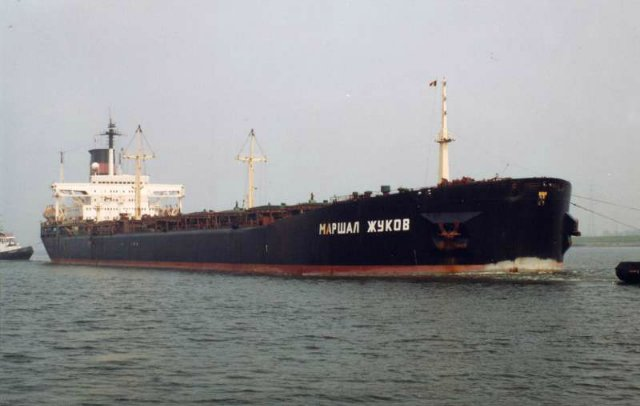
\includegraphics[scale=0.5]{Figs/marshl_jukov.jpg}
    \caption{Судно <<Маршал Жуков>>}
    \label{fig:jukov}
\end{figure}

И подобные явления, как оказалось, описывались и задолго до Франклина. В своей <<естественной истории>> Плиний Старший говорит о похожем явлении \cite{Plinii}. Позднее <<мертвая вода>> была воспроизведена в лабораторных условиях исследователями из франции \cite{deadWater}. Запись эксперимента доступна на видеохостинге youtube \cite{deadWaterVideo}.


Математически описать возникновение внутренних волн можно записав уравнение для сил, которые действуют на выведенную из равновесия частицу жидкости(Рис. \ref{fig:Forces}):

\begin{equation}
    m_b \vec{a}_b = \vec{P} + \vec{G}
\end{equation}
где $\vec{P}=\rho_w \vec{g} S \cdot h$ это сила Архимеда, $\rho_w$ плотность жидкости того слоя на котором находится частица, $\vec{g}$ -- ускорение свободного падения, $S$ -- площадь стороны частицы, $h$  -- глубина. $\vec{G} = \rho_b \vec{g} S \cdot h$,  $\rho_b$ -- плотность частицы жидкости.

В проекции на вертикальную ось:

\begin{equation}
    \frac{d^2 \xi}{dt^2} = \frac{(\rho_w-\rho_b)}{\rho_b}\cdot g
\end{equation}

Тут $\xi$ будет обозначать отклонение от положения равновесия $z_0$, тогда очевидно что плотность воды вокруг частицы и плотность частицы будет равна в положении равновесия при $\xi=0$ $\rho_w(z_0)=\rho_b$ тогда уравнение можно переписать:

\begin{equation}
    \frac{d^2 \xi}{dt^2} = \frac{\rho_w(z_0+\xi)-\rho_b}{\rho_b}\cdot g
    \label{eq:beg}
\end{equation}

Введем переобозначение, $z=z_0+\xi$ тогда правая часть уравнения запишется $$\frac{\rho_w(z_0+\xi)-\rho_b}{\rho_b}\cdot g = \frac{\rho_w(z)-\rho_w(z_0)}{\rho_w(z_0)}\cdot g = \frac{1}{\rho(z_0)} \frac{\rho_w(z)-\rho_w(z_0)}{z-z_0}\cdot(z-z_0) g$$

При достаточно малом $t$ отклонении от положения равновесия $z$ будет также мало, что дает нам возможность перейти к производной по $z$, а $\rho_w$ переобозначим как $\rho$ и окончательно запишем:

\begin{equation}
    \frac{d^2 \xi}{dt^2} =\frac{1}{\rho} \frac{d\rho}{z}\xi \cdot g
\end{equation}

Решение этого дифференциального уравнения ищется в виде периодической функции, это значит, что частица совершает колебания около своего положения равновесия:

\begin{equation}
    \xi(t)=A cos(\omega t + \phi)
\end{equation}

подставим выражения $\xi(t)$ в уравнение:

\begin{equation}
    \ddot{\xi} = - A \omega^2 cos(\omega t + \phi )
\end{equation}

или если выразить правую часть через $\xi$

\begin{equation}
    \ddot{\xi} = - \omega^2  \xi
    \label{eq:final}
\end{equation}

Подставим (\ref{eq:final}) в (\ref{eq:beg}):

\begin{equation}
    -\omega^2 \xi = \frac{1}{\rho_0}\cdot \frac{d \rho}{d z} \xi g
\end{equation}

Выразим частоту колебаний частицы:

\begin{equation}
    \omega(z) = N(z) = \sqrt{- \frac{g}{\rho_0}\cdot\frac{d \rho(z)}{dz}}
\end{equation}

Эта частота называется частота плавучести или Частота Брента — Вяйсяля. В океане она составляет величину порядка $10^{-3}$ $\frac{1}{\textup{с}}$ \cite{King2012}.

\begin{figure}
    \centering
    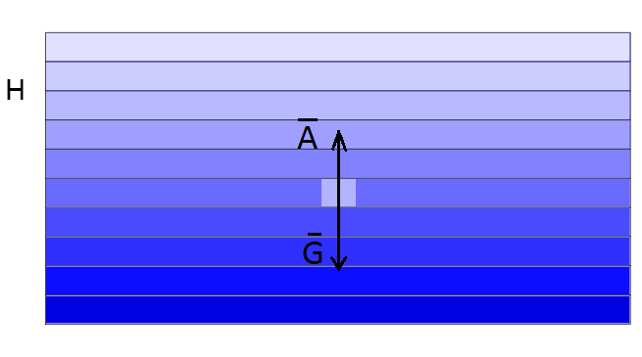
\includegraphics[scale=0.8]{Figs/Forces.png}
    \caption{Схематичное представление сил действующие на частицу выведенную из равновесия в стратифицированной жидкости, цветом показана плотность.}
    \label{fig:Forces}
\end{figure}

\begin{figure}
    \centering
    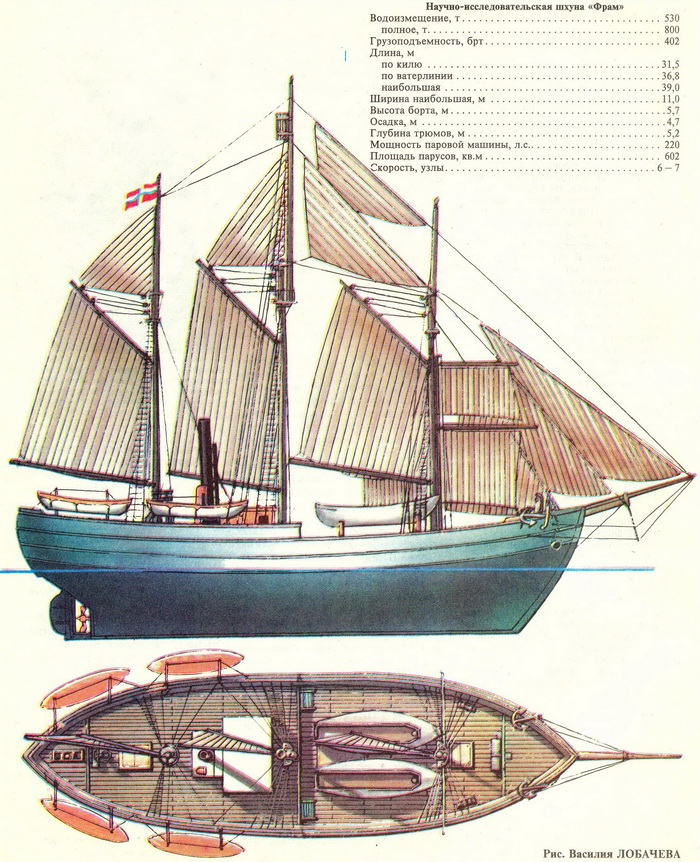
\includegraphics[width=1\textwidth]{Figs/FRAM.jpg}
    \caption{Исследовательское судно <<Фрам>>}
    \label{fig:fram}
\end{figure}

\begin{figure}
    \centering
    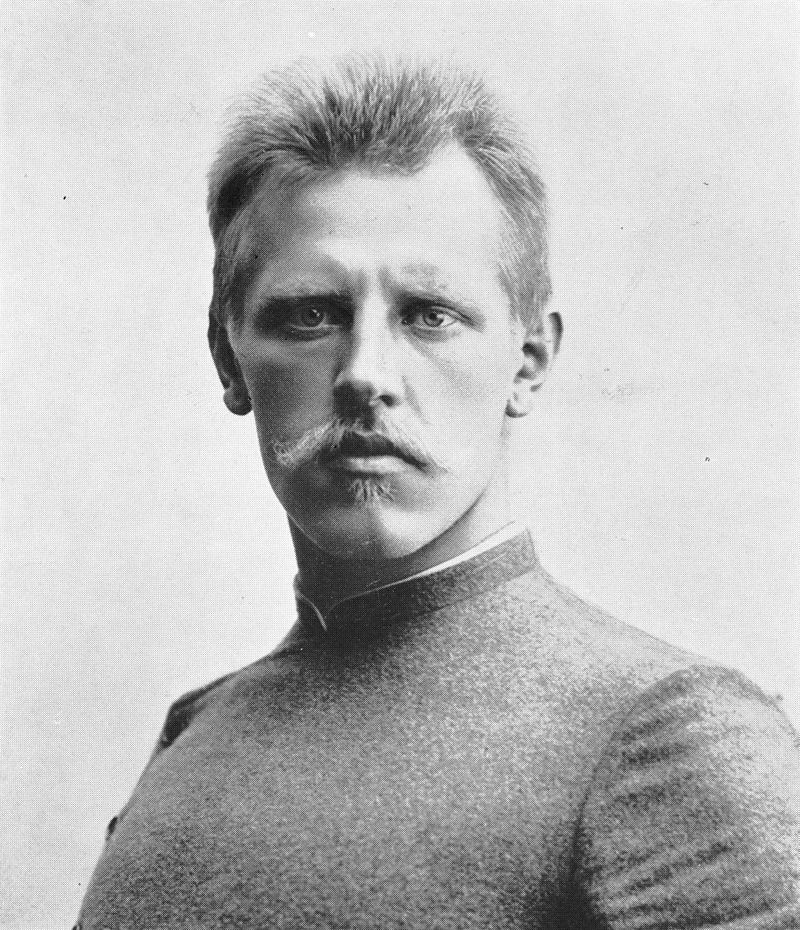
\includegraphics[scale=2.5]{Figs/800px-Fridtjof_Nansen.jpg}
    \caption{Фритьоф Ведель-Ярлсберг Нансен (1861-1930)}
    \label{fig:Nansen}
\end{figure}

\section{Обзор литературы}

Внутренние волны очень распространенное явление в океане. Существуют они благодаря перепадам плотности на разной глубине, сила плавучести играет роль восстанавливающей силы. Океаны являются одним из естественных примеров стратифицированных сред. Основные источники внутренних волн в океане это приливные эффекты, которые сопряжены с движением Земли относительно Солнца и Луны относительно Земли.

Внутренние волны активно взаимодействуют с другими океаническими структурами \cite{Rainville2006} и с неровностями океанического дна \cite{DAUXOIS1999}. Процессы перемещения внутренних волн их взаимодействия друг с другом и океаническими структурами различных масштабов образуют собой явление называемое энергетическим каскадом\cite{Garrett1972}. Энергетический каскад способствует поддержанию глобальной океанической циркуляции и перемешиванию\cite{Nikurashin2012,Munk1998}. Тем не менее, механизмы вносящие крупномасштабный приливный вклад в движение внутренних волн недостаточно понятны \cite{Ivey2008,Polzin1997} и каскадный процесс остается одной из фундаментальных проблем современной океанографии. Главным образом остаются вопросы связи крупномасштабных и мелкомасштабных явлений.

Одним из объяснений этой связи могут послужить аттракторы внутренних гравитационных волн. Это явление, при котором внутренние волны многократно отражаясь от поверхности океана, его дна и неровностей движутся по замкнутым орбитам. Возникновение такого явление возможно лишь в том случае, когда на дне океана имеются определенные комбинации геометрических неровностей. Аттракторы передают кинетическую энергию крупномасштабных эффектов, такие как приливы и внутренние волны большой длинны к мелкомасштабным явлениям волновой турбулентности и перемешиванию. Происходит это благодаря явлению фокусировки, в результате которого длинна внутренних волн уменьшается, но увеличивается амплитуда.

Возможность возникновения аттракторов в океане с реальной геометрией дна уже исследовалась\cite{Tang2010}. Например, топология северной части хребта Лусона имеет соответствующую геометрию. Эксперименты~\cite{ECHEVERRI2011} подтверждают возможность образования аттракторов внутренних волн. Кроме того при моделировании внутренних волн в условиях случайного разреза геометрии океанического дна, был сделан вывод, что с немалой вероятностью возможны возникновения аттракторов по одному на каждую сотню километров океанического дна \cite{Guo2015}. Тем не менее стоит отметить, что на данный момент нет свидетельств наблюдаемых волновых аттракторов. Возможно это связано с тем, что теоретические работы\cite{Guo2015} относятся к двумерному океану, но также существуют трехмерные конфигурации геометрий в которых возможны существования трехмерных волновых аттракторов\cite{Drijfhout2007,Manders2004}. Кроме того, в теоретическом представлении аттракторов внутренних волн не учитывается шероховатость поверхностей отражения. Однако надежность теоретических соображений о возможности существования трехмерных аттракторов была экспериментально проверена\cite{Hazewinkel2010}. Кроме того волновые явления в океане часто имеют целый спектр частот\cite{Garrett1972}, в то время как многочисленные эксперименты проводятся лишь с монохроматическим источником внутренних волн.

Предполагается, что аттракторы могут влиять не только на перемешивание, но и на движение мелких животных, явление седиментации и эрозию прибрежных конструкций.

Работы по фокусировке внутренних волн и образованию устойчивых аттракторов ведутся с конца двадцатого века. Первое теоретическое предсказание аттракторов было сделано Лео Маасом в 1995 году\cite{Maas1995}. Через два года последовали экспериментальные исследования этого явления, теоретические результаты были воспроизведены\cite{Maas1997}. Эффекты фокусировки характерны не только для стратифицированной жидкости, но и для вращающихся \cite{articleMaas2003,Veronis1970}. В дальнейшем теоретические основы явления были пересмотрены на основании данных эксперимента\cite{Lam2008}.

Вместе с развитием вычислительной техники развивались и инструменты численного моделирования физических явлений. Во втором десятилетии двадцать первого века стало возможным численное моделирование трехмерных аттракторов внутренних волн. Первая удачная попытка была предпринята с использованием метода спектральных элементов\cite{Brouzet2016,Brouzet_2016}. При сравнении с экспериментом ошибка численного моделирования составила не больше 10\%. Также была предпринята попытка моделирования аттрактора внутренних волн с помощью метода конечного объема\cite{Brouzet2014}. Количественно воспроизвести результаты, полученные с помощью метода спектральных элементов не удалось.
Традиционно для моделирования аттракторов применяются уравнения Навье-Стокса в приближении Буссинеска. Однако существует ряд работ, где вместо классического подхода используется квазигидродинамический\cite{ElizarBook}. Квазигидродинамические уравнения позволяют добиться большей точности\cite{Kraposhin20182} при моделировании методом конечного объема.

Результаты работы представляют собой интерес для приложений в океанологии, экологии, биологии, астрофизики и вращающихся технических систем. 

\paragraph{Цель работы} -- изучение явления бигармонического аттрактора, которое возникает при воздействии на стратифицированную жидкость двухчастотным волнопродуктором.  
С этой целбю были посталены следующие задачи \textbf{задачи}:

\begin{itemize}

  \item Нахождение интервала частот внешних воздействий, при которых возникает аттрактор внутренних волн.
  
  % Изучение интервалов частот внешних воздействий и других параметров, при которых происходит аккумуляция волновой энергии, в частности волновых аттракторов.

%    \item Нахождение частотных параметров приводящих к образованию аттракторов в резервуаре.
    
  % \item Обзор существующих методов моделирования аттракторов внутренних волн. Выявление их достоинств и недостатков.
    
  \item Реализация численных экспериментов с помощью двух подходов: спектрально-элементного и конечно-объемного.

  \item Разработка новой программы для моделирования аттракторов внутренних волн на основе квазигидродинамического подхода.
    
  \item Верификация результатов численного моделирования.

  \item Описание особенностей волновых режимов при бигармоническом воздействии и значительно отличающихся частотах воздействия и малых амплитудах.

  \item Описание особенностей волновых режимов при бигармоническом воздействии, близких частотах воздействия и малых амплитудах.
    
  \item Описание особенностей нелинейных волновых режимов при бигармоническом воздействии и близких частотах воздействия.

  \item Сравнение динамики средней кинетической энергии и пульсации кинетической энергии для монохроматического режима и различных бигармонических режимов.
    

    
\end{itemize}

\paragraph{Методы решения поставленных задач}

Для решения поставленых задач были использованы методы математического моделирования механики сплшных сред, такие как метод спектральных элементов и метд конечного объема. Для предсказания формы аттрактора внутренних волн использовался метод трассировки лучей. Для анализа данных использовался метод построения частотно-временных диаграмм при помощи быстрого преобразования Фурье.

\paragraph{Научная новизна работы} выражается в конкретных реузьтатах:
\begin{enumerate}[1.]
  \item Получены аналитические выражения для границ частотного интервала существования аттракторов внутренних волн.% конфигурации (1,1). 
    
  \item Получена геометрия течения, которая возникает в трапециевидном резервуаре, наполненном стратифицированной жидкостью при воздействии на жидкость внешними возмущениями с двумя различными частотами. 
    
  \item Проведён анализ результатов моделирования аттрактора внутренних волн при бигармоническом воздействии, полученных с помощью метода спектральных элементов. Для различных комбинаций возмущающих частот построен спектр, частотно-временная диаграмма и зависимость средней кинетической энергии от времени. 
    
  \item Реализован квазигидродинамический подход на базе метода конечного элемента. Проведено сопоставление результатов моделирования методов конечных объемов и методом спектральных элементов.
\end{enumerate}

\paragraph{Достоверность результатов}

Достоверность полученных результатов гарантируется строгой математической постановкой, верификацией и валидацией разработанного алгоритма для решения поставленной задачи.

% \paragraph{Объектом исследования} являются волновые режимы возникающие %в естественных условиях 
% при двух источниках внешних воздействий на стратифицированную жидкость в трапециевидном резервуаре.

% %Приложения включают в себя задачи океанологии, астрофизики и технических вращающихся систем при периодических воздействиях. 

% %\paragraph{В исследовании использованы следующие методы:}
% \begin{itemize}
%   \item [    В исследовании использованы \textbf{
% методы:}]
%   \item методы численного моделирования конечного объема;
%   \item метод спектральных элементов;
%   \item метод трассировки лучей;
%   \item Фурье анализ полученных результатов, в том числе по скользящему окну;
%   \item разложение по эмпирическим модам;
% \end{itemize}

% % В работе рассматриваются резервуары в форме трапеций различных конфигураций, заполненных стратифицированной жидкостью. Одна из стенок резервуара представляет собой волнопродуктор, который порождает внутренние волны в стратифицированной среде. Результаты разработки предоставляют возможность проводить моделирование аттракторов внутренних волн в условиях сложной геометрии и неортогональных сетках. 



\paragraph{Практическая значимость} 

Ранее эксперименты по исследованию бигармонических аттракторов, как численные так и натурные, не проводились. Теоретически, бигармонический аттрактор представляет собой новую устойчивую структуру, которая образуется в стратифицированной жидкости при воздействии на нее периодическим двухчастотным возмущением.

Положения и выводы диссертационного исследования могут быть использованы для подбора параметров  волнового аттрактора в лабораторных условиях или при численном моделировании. Среди возможных приложений результатов работы — задачи моделирования аттракторов внутренних волн на сложных геометриях, задачи моделирования течений со сложным спектром частотных воздействий на стратифицированную жидкость. Работа является первым шагом к моделированию течений, возникающих в условиях, приближенных к реальным океаническим, что позволит выяснить форму и вид природных аттракторов внутренних волн. Комбинация методов конечного объёма и квазигидродинамических уравнений позволила добиться существенного улучшения в точности моделирования и дала инструмент к  усложнению геометрии расчётной области. Разработанная программа может быть применена не только к задачам моделирования аттрактора, но и к другим задачам гидродинамики с дозвуковыми и трансзвуковыми скоростями.

\paragraph{На защиту выносятся следующие положения:}
\begin{itemize}

  \item Найдены аналитические выражения для границ диапазонов частот колебаний волнопродуктора, которые способны порождать аттракторы.

  \item Показано, что при значительном отличии частот внешних воздействий и малых амплитудах воздействий волновой режим представляет из себя совокупность независимо существующих волновых аттракторов.

  \item Показано, что при близких частотах внешних воздействий и малых амплитудах возникает режим с биениями, характерной особенностью которых является малая амплитуда пульсаций на убывающем склоне огибающей.

  \item Показано, что при близких частотах внешних воздействий и средних амплитудах возникают биения, на одном цикле которых успевает происходит переход к турбулентности через триадные резонансы, и реламинаризация.
    
  \item Обнаружено наличие фазового сдвига между биениями на волнопродукторе и биениями средней кинетической энергии во всем объеме.
    
%   \item 
%     Сравнение динамики средней кинетической энергии и пульсации кинетической энергии для монохроматического режима и различных бигармонических режимов указывает на то, что на убывающем склоне огибающей большая доля кинетической энергии переходит в бегущие волны по сравнению с возрастающей фазой.

  \item Разработана и верифицирована новая программа для моделирования аттракторов внутренних волн и в целом динамики стратифицированных сред.
    
%  \item Реализация численных экспериментов с помощью двух подходов: спектрально-элементного и конечно-объемного.

%  \item Проведена верификация результатов численного моделирования.
%    Проведение численных экспериментов различными методами.
    
%  \item Количественный анализ результатов численных экспериментов. 
    
%  \item Верификация разработанной программы.
    
\end{itemize}

\paragraph{Личный вклад автора}

Исследования, результаты которых выносятся на защиту, были получены лично соискателем. Соискатель аналитически нашел диапазон частот внешнего воздействия при которых образуется аттрактор внутренних волн. Соискатель подобрал параметры эксперемента, провел расчеты и проанализировал полученные данные. Также принимал непосредственное участие в разработке реализации квазигидродинамического подхода на базе открытого программного комлекса OpenFOAM. Научный руководитель И. Н. Сибгатуллин поставил первоначальную задачу и участввал в обсуждении результатов. 

\paragraph{Аппробация работы}

Материалы диссертации представлялись на различных конференциях, семинарах, как российсих так и международных:


\begin{itemize}
  \item Открытая международная конференция ИСП РАН им. В.П.Иванникова. 5-6 декабря 2019 г, г. Москва Главное здание Российской академии наук (устный доклад).
  \item Международная конференция «Суперкомпьютерные технологии математического моделирования» (СКТеММ’19), 19-21 июня 2019, г. Москва (устный доклад).
  \item 13th OpenFOAM Workshop, Shanghai, China, Китай, 24-29 июня 2018 (устный доклад).
  \item XXIII международная конференция «Нелинейные задачи теории гидродинамической устойчивости и турбулентность». 25 февраля - 4 марта 2018, Московская область, г. Звенигород (стендовый доклад).
  \item Рязанов Д.А. Открытая конференция ИСП РАН им. В.П. Иванникова. 30 ноября - 1 декабря 2017 г. Москва главное здание Российской академии наук (стендовый доклад).
\end{itemize}

\paragraph{Публикации}

По результатам диссертации опубликовано 12 научныйх работ, входящих в базы данных и системы цитирования РИНЦ, Scopus, Web of Science, 2 из них входят в Перечень рецензируемых научных изданий, рекомендованных Высшей раттестационной комиссией. Зарегестрирована программа для ЭВМ.

\paragraph{Сутрктура и объем диссертации}

% В ходе работ был разработан программный продукт, который подлежал государственной регистрации № 2018663951.

% \Introduction

Важной задачей изучения аттракторов внутренних волн с помощью численных методов является обеспечение возможности проводить численные эксперименты с геометрией, приближенной к геометрии реального дна океана. Выполнение этой задачи ускорило и удешевило бы процесс непостредственного поиска аттракторов внутренних волн в океане, и изучение влияния аттркаторов на турбулентные режимы. Метод спектральных элементов, который обеспечивает достаточную точность воспроизведения результатов эксперимента, ограничен в своей реализации сложностью геометрии расчетной области. В свою очередь, метод конечного объема позволяет работать со сложной геометрией, которая способна имитировать поверхность океанического дна, но стандартные реализации не обладают достаточной точностью. Кроме того, монохроматический источника возмущений может не описывать реальные внешние воздействия. Зачастую, при моделировании явлений, связанных с образованием аттракторов в реальных условиях, необходимо учитывать несколько приливных воздействий \cite{Garrett1972} и изменение стратификации.

Явление внутренних волн представляется собой нарушение состояние равновесия на границе раздела водяных слоев различной плотности. Выеденные из равновесия частицы жидкости начинают совершать колебания под действием силы тяжести и силы Архимеда.

Считается установленным, что впервые внутренние волны наблюдал американский ученый Франклин в восемнадцатом веке с помощью простой экспериментальной установки. Она представляла собой емкость, заполненную несмешивающимися жидкостями различной полости~\cite{Sudolski}. Однако в конце восемнадцатого века вблизи полуострова Таймыр произошло событие, которое заострило внимание научного сообщества на этом интересном явлении. В то время в этом районе пролегал маршрут исследовательского судна <<Фрам>>(Рис. \ref{fig:fram}) под руководством Фритьофа Нансена (Рис. \ref{fig:Nansen}).

Однажды во время штиля судно остановилось. Скорость его движения резко снизилась.  «чтобы пройти то небольшое расстояние, которое мы и на веслах прошли бы в полчаса или того меньше, «Фраму» понадобилась целая вахта», -- как писал сам Нансен. При этом исследователь отмечал, что вода на поверхности была пресной, потому как натекла с оттаявших ледников. А на глубине сравнимой с осадкой судна, резко становилась соленой. Позднее его записи послужили стимулом для теоретических исследований этого явления. В итоге было установлено, что почти вся энергия судового двигателя сдвигает не судно, а образует волны на поверхности раздела между слоями пресной и соленой воды. Это явление получило название <<мертвая вода>>.

Также существует еще одно свидетельство этого явления. Теплоход «Маршал Жуков» при проходе пролива Дарданеллы угодил в <<мертвую воду>> летом 1981 года. Уже в сентябре в отраслевой газете <<черноморец>> капитан-наставник Александр Косилов подробно описал как в течении четырех суток судно, держащее курс из Канады в Новороссийск, боролось с феноменом. Согласно комментариям руководителя аналитико-исследовательской группы управления инвестиций и проектов ОАО «Новошип», кандидата технических наук, профессора кафедры судовождения ГМУ им. адмирала Ф.Ф. Ушакова Юрия Пескова современные суда в значительной степени подвержены влиянию подобных явлений\cite{MorVest}. На то есть причины:

\begin{itemize}
    \item Экономия топлива вынуждает снижать скоростные режимы
    \item Борьба за уменьшение углекислых выбросов предписывает снижать мощность двигателя
\end{itemize}


\begin{figure}
    \centering
    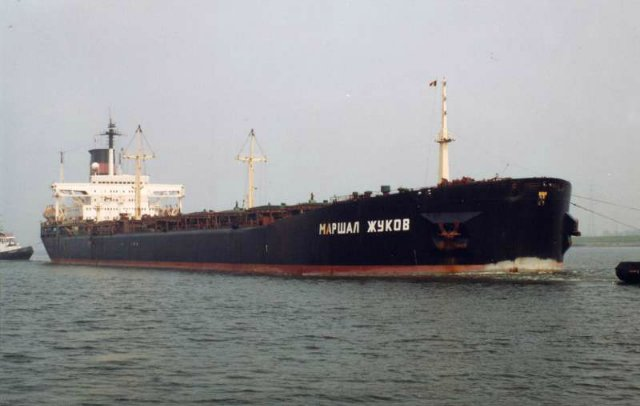
\includegraphics[scale=0.5]{Figs/marshl_jukov.jpg}
    \caption{Судно <<Маршал Жуков>>}
    \label{fig:jukov}
\end{figure}

И подобные явления, как оказалось, описывались и задолго до Франклина. В своей <<естественной истории>> Плиний Старший говорит о похожем явлении \cite{Plinii}. Позднее <<мертвая вода>> была воспроизведена в лабораторных условиях исследователями из франции \cite{deadWater}. Запись эксперимента доступна на видеохостинге youtube \cite{deadWaterVideo}.


Математически описать возникновение внутренних волн можно записав уравнение для сил, которые действуют на выведенную из равновесия частицу жидкости(Рис. \ref{fig:Forces}):

\begin{equation}
    m_b \vec{a}_b = \vec{P} + \vec{G}
\end{equation}
где $\vec{P}=\rho_w \vec{g} S \cdot h$ это сила Архимеда, $\rho_w$ плотность жидкости того слоя на котором находится частица, $\vec{g}$ -- ускорение свободного падения, $S$ -- площадь стороны частицы, $h$  -- глубина. $\vec{G} = \rho_b \vec{g} S \cdot h$,  $\rho_b$ -- плотность частицы жидкости.

В проекции на вертикальную ось:

\begin{equation}
    \frac{d^2 \xi}{dt^2} = \frac{(\rho_w-\rho_b)}{\rho_b}\cdot g
\end{equation}

Тут $\xi$ будет обозначать отклонение от положения равновесия $z_0$, тогда очевидно что плотность воды вокруг частицы и плотность частицы будет равна в положении равновесия при $\xi=0$ $\rho_w(z_0)=\rho_b$ тогда уравнение можно переписать:

\begin{equation}
    \frac{d^2 \xi}{dt^2} = \frac{\rho_w(z_0+\xi)-\rho_b}{\rho_b}\cdot g
    \label{eq:beg}
\end{equation}

Введем переобозначение, $z=z_0+\xi$ тогда правая часть уравнения запишется $$\frac{\rho_w(z_0+\xi)-\rho_b}{\rho_b}\cdot g = \frac{\rho_w(z)-\rho_w(z_0)}{\rho_w(z_0)}\cdot g = \frac{1}{\rho(z_0)} \frac{\rho_w(z)-\rho_w(z_0)}{z-z_0}\cdot(z-z_0) g$$

При достаточно малом $t$ отклонении от положения равновесия $z$ будет также мало, что дает нам возможность перейти к производной по $z$, а $\rho_w$ переобозначим как $\rho$ и окончательно запишем:

\begin{equation}
    \frac{d^2 \xi}{dt^2} =\frac{1}{\rho} \frac{d\rho}{z}\xi \cdot g
\end{equation}

Решение этого дифференциального уравнения ищется в виде периодической функции, это значит, что частица совершает колебания около своего положения равновесия:

\begin{equation}
    \xi(t)=A cos(\omega t + \phi)
\end{equation}

подставим выражения $\xi(t)$ в уравнение:

\begin{equation}
    \ddot{\xi} = - A \omega^2 cos(\omega t + \phi )
\end{equation}

или если выразить правую часть через $\xi$

\begin{equation}
    \ddot{\xi} = - \omega^2  \xi
    \label{eq:final}
\end{equation}

Подставим (\ref{eq:final}) в (\ref{eq:beg}):

\begin{equation}
    -\omega^2 \xi = \frac{1}{\rho_0}\cdot \frac{d \rho}{d z} \xi g
\end{equation}

Выразим частоту колебаний частицы:

\begin{equation}
    \omega(z) = N(z) = \sqrt{- \frac{g}{\rho_0}\cdot\frac{d \rho(z)}{dz}}
\end{equation}

Эта частота называется частота плавучести или Частота Брента — Вяйсяля. В океане она составляет величину порядка $10^{-3}$ $\frac{1}{\textup{с}}$ \cite{King2012}.

\begin{figure}
    \centering
    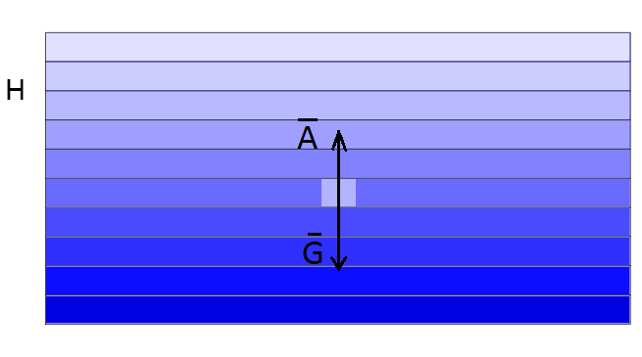
\includegraphics[scale=0.8]{Figs/Forces.png}
    \caption{Схематичное представление сил действующие на частицу выведенную из равновесия в стратифицированной жидкости, цветом показана плотность.}
    \label{fig:Forces}
\end{figure}

\begin{figure}
    \centering
    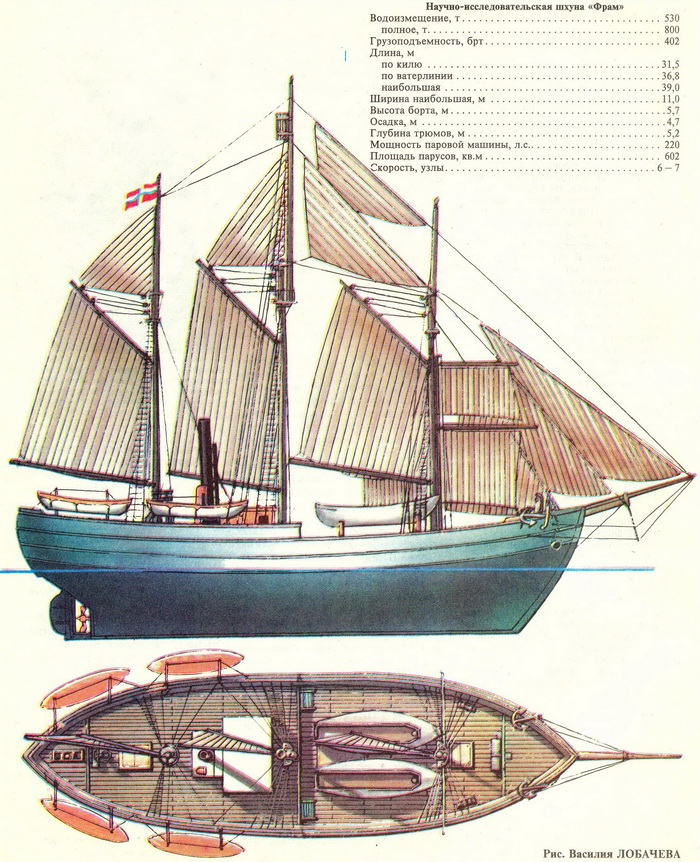
\includegraphics[width=1\textwidth]{Figs/FRAM.jpg}
    \caption{Исследовательское судно <<Фрам>>}
    \label{fig:fram}
\end{figure}

\begin{figure}
    \centering
    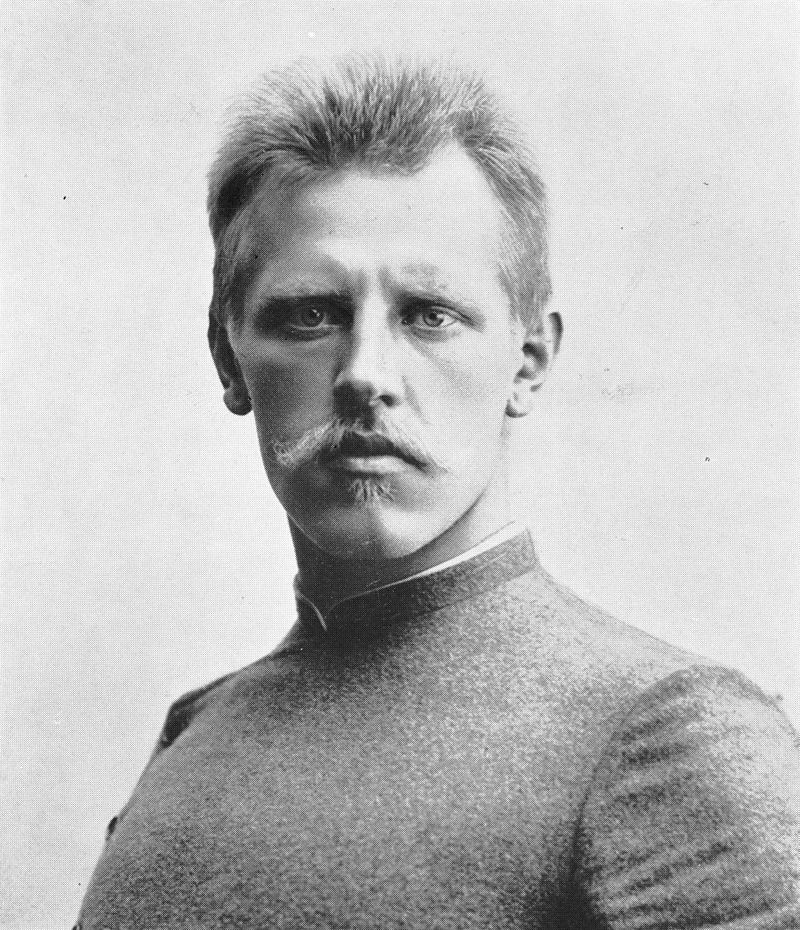
\includegraphics[scale=2.5]{Figs/800px-Fridtjof_Nansen.jpg}
    \caption{Фритьоф Ведель-Ярлсберг Нансен (1861-1930)}
    \label{fig:Nansen}
\end{figure}

\section{Обзор литературы}

Внутренние волны очень распространенное явление в океане. Существуют они благодаря перепадам плотности на разной глубине, сила плавучести играет роль восстанавливающей силы. Океаны являются одним из естественных примеров стратифицированных сред. Основные источники внутренних волн в океане это приливные эффекты, которые сопряжены с движением Земли относительно Солнца и Луны относительно Земли.

Внутренние волны активно взаимодействуют с другими океаническими структурами \cite{Rainville2006} и с неровностями океанического дна \cite{DAUXOIS1999}. Процессы перемещения внутренних волн их взаимодействия друг с другом и океаническими структурами различных масштабов образуют собой явление называемое энергетическим каскадом\cite{Garrett1972}. Энергетический каскад способствует поддержанию глобальной океанической циркуляции и перемешиванию\cite{Nikurashin2012,Munk1998}. Тем не менее, механизмы вносящие крупномасштабный приливный вклад в движение внутренних волн недостаточно понятны \cite{Ivey2008,Polzin1997} и каскадный процесс остается одной из фундаментальных проблем современной океанографии. Главным образом остаются вопросы связи крупномасштабных и мелкомасштабных явлений.

Одним из объяснений этой связи могут послужить аттракторы внутренних гравитационных волн. Это явление, при котором внутренние волны многократно отражаясь от поверхности океана, его дна и неровностей движутся по замкнутым орбитам. Возникновение такого явление возможно лишь в том случае, когда на дне океана имеются определенные комбинации геометрических неровностей. Аттракторы передают кинетическую энергию крупномасштабных эффектов, такие как приливы и внутренние волны большой длинны к мелкомасштабным явлениям волновой турбулентности и перемешиванию. Происходит это благодаря явлению фокусировки, в результате которого длинна внутренних волн уменьшается, но увеличивается амплитуда.

Возможность возникновения аттракторов в океане с реальной геометрией дна уже исследовалась\cite{Tang2010}. Например, топология северной части хребта Лусона имеет соответствующую геометрию. Эксперименты~\cite{ECHEVERRI2011} подтверждают возможность образования аттракторов внутренних волн. Кроме того при моделировании внутренних волн в условиях случайного разреза геометрии океанического дна, был сделан вывод, что с немалой вероятностью возможны возникновения аттракторов по одному на каждую сотню километров океанического дна \cite{Guo2015}. Тем не менее стоит отметить, что на данный момент нет свидетельств наблюдаемых волновых аттракторов. Возможно это связано с тем, что теоретические работы\cite{Guo2015} относятся к двумерному океану, но также существуют трехмерные конфигурации геометрий в которых возможны существования трехмерных волновых аттракторов\cite{Drijfhout2007,Manders2004}. Кроме того, в теоретическом представлении аттракторов внутренних волн не учитывается шероховатость поверхностей отражения. Однако надежность теоретических соображений о возможности существования трехмерных аттракторов была экспериментально проверена\cite{Hazewinkel2010}. Кроме того волновые явления в океане часто имеют целый спектр частот\cite{Garrett1972}, в то время как многочисленные эксперименты проводятся лишь с монохроматическим источником внутренних волн.

Предполагается, что аттракторы могут влиять не только на перемешивание, но и на движение мелких животных, явление седиментации и эрозию прибрежных конструкций.

Работы по фокусировке внутренних волн и образованию устойчивых аттракторов ведутся с конца двадцатого века. Первое теоретическое предсказание аттракторов было сделано Лео Маасом в 1995 году\cite{Maas1995}. Через два года последовали экспериментальные исследования этого явления, теоретические результаты были воспроизведены\cite{Maas1997}. Эффекты фокусировки характерны не только для стратифицированной жидкости, но и для вращающихся \cite{articleMaas2003,Veronis1970}. В дальнейшем теоретические основы явления были пересмотрены на основании данных эксперимента\cite{Lam2008}.

Вместе с развитием вычислительной техники развивались и инструменты численного моделирования физических явлений. Во втором десятилетии двадцать первого века стало возможным численное моделирование трехмерных аттракторов внутренних волн. Первая удачная попытка была предпринята с использованием метода спектральных элементов\cite{Brouzet2016,Brouzet_2016}. При сравнении с экспериментом ошибка численного моделирования составила не больше 10\%. Также была предпринята попытка моделирования аттрактора внутренних волн с помощью метода конечного объема\cite{Brouzet2014}. Количественно воспроизвести результаты, полученные с помощью метода спектральных элементов не удалось.
Традиционно для моделирования аттракторов применяются уравнения Навье-Стокса в приближении Буссинеска. Однако существует ряд работ, где вместо классического подхода используется квазигидродинамический\cite{ElizarBook}. Квазигидродинамические уравнения позволяют добиться большей точности\cite{Kraposhin20182} при моделировании методом конечного объема.

Результаты работы представляют собой интерес для приложений в океанологии, экологии, биологии, астрофизики и вращающихся технических систем. 

\paragraph{Цель работы} -- изучение явления бигармонического аттрактора, которое возникает при воздействии на стратифицированную жидкость двухчастотным волнопродуктором.  
С этой целбю были посталены следующие задачи \textbf{задачи}:

\begin{itemize}

  \item Нахождение интервала частот внешних воздействий, при которых возникает аттрактор внутренних волн.
  
  % Изучение интервалов частот внешних воздействий и других параметров, при которых происходит аккумуляция волновой энергии, в частности волновых аттракторов.

%    \item Нахождение частотных параметров приводящих к образованию аттракторов в резервуаре.
    
  % \item Обзор существующих методов моделирования аттракторов внутренних волн. Выявление их достоинств и недостатков.
    
  \item Реализация численных экспериментов с помощью двух подходов: спектрально-элементного и конечно-объемного.

  \item Разработка новой программы для моделирования аттракторов внутренних волн на основе квазигидродинамического подхода.
    
  \item Верификация результатов численного моделирования.

  \item Описание особенностей волновых режимов при бигармоническом воздействии и значительно отличающихся частотах воздействия и малых амплитудах.

  \item Описание особенностей волновых режимов при бигармоническом воздействии, близких частотах воздействия и малых амплитудах.
    
  \item Описание особенностей нелинейных волновых режимов при бигармоническом воздействии и близких частотах воздействия.

  \item Сравнение динамики средней кинетической энергии и пульсации кинетической энергии для монохроматического режима и различных бигармонических режимов.
    

    
\end{itemize}

\paragraph{Методы решения поставленных задач}

Для решения поставленых задач были использованы методы математического моделирования механики сплшных сред, такие как метод спектральных элементов и метд конечного объема. Для предсказания формы аттрактора внутренних волн использовался метод трассировки лучей. Для анализа данных использовался метод построения частотно-временных диаграмм при помощи быстрого преобразования Фурье.

\paragraph{Научная новизна работы} выражается в конкретных реузьтатах:
\begin{enumerate}[1.]
  \item Получены аналитические выражения для границ частотного интервала существования аттракторов внутренних волн.% конфигурации (1,1). 
    
  \item Получена геометрия течения, которая возникает в трапециевидном резервуаре, наполненном стратифицированной жидкостью при воздействии на жидкость внешними возмущениями с двумя различными частотами. 
    
  \item Проведён анализ результатов моделирования аттрактора внутренних волн при бигармоническом воздействии, полученных с помощью метода спектральных элементов. Для различных комбинаций возмущающих частот построен спектр, частотно-временная диаграмма и зависимость средней кинетической энергии от времени. 
    
  \item Реализован квазигидродинамический подход на базе метода конечного элемента. Проведено сопоставление результатов моделирования методов конечных объемов и методом спектральных элементов.
\end{enumerate}

\paragraph{Достоверность результатов}

Достоверность полученных результатов гарантируется строгой математической постановкой, верификацией и валидацией разработанного алгоритма для решения поставленной задачи.

% \paragraph{Объектом исследования} являются волновые режимы возникающие %в естественных условиях 
% при двух источниках внешних воздействий на стратифицированную жидкость в трапециевидном резервуаре.

% %Приложения включают в себя задачи океанологии, астрофизики и технических вращающихся систем при периодических воздействиях. 

% %\paragraph{В исследовании использованы следующие методы:}
% \begin{itemize}
%   \item [    В исследовании использованы \textbf{
% методы:}]
%   \item методы численного моделирования конечного объема;
%   \item метод спектральных элементов;
%   \item метод трассировки лучей;
%   \item Фурье анализ полученных результатов, в том числе по скользящему окну;
%   \item разложение по эмпирическим модам;
% \end{itemize}

% % В работе рассматриваются резервуары в форме трапеций различных конфигураций, заполненных стратифицированной жидкостью. Одна из стенок резервуара представляет собой волнопродуктор, который порождает внутренние волны в стратифицированной среде. Результаты разработки предоставляют возможность проводить моделирование аттракторов внутренних волн в условиях сложной геометрии и неортогональных сетках. 



\paragraph{Практическая значимость} 

Ранее эксперименты по исследованию бигармонических аттракторов, как численные так и натурные, не проводились. Теоретически, бигармонический аттрактор представляет собой новую устойчивую структуру, которая образуется в стратифицированной жидкости при воздействии на нее периодическим двухчастотным возмущением.

Положения и выводы диссертационного исследования могут быть использованы для подбора параметров  волнового аттрактора в лабораторных условиях или при численном моделировании. Среди возможных приложений результатов работы — задачи моделирования аттракторов внутренних волн на сложных геометриях, задачи моделирования течений со сложным спектром частотных воздействий на стратифицированную жидкость. Работа является первым шагом к моделированию течений, возникающих в условиях, приближенных к реальным океаническим, что позволит выяснить форму и вид природных аттракторов внутренних волн. Комбинация методов конечного объёма и квазигидродинамических уравнений позволила добиться существенного улучшения в точности моделирования и дала инструмент к  усложнению геометрии расчётной области. Разработанная программа может быть применена не только к задачам моделирования аттрактора, но и к другим задачам гидродинамики с дозвуковыми и трансзвуковыми скоростями.

\paragraph{На защиту выносятся следующие положения:}
\begin{itemize}

  \item Найдены аналитические выражения для границ диапазонов частот колебаний волнопродуктора, которые способны порождать аттракторы.

  \item Показано, что при значительном отличии частот внешних воздействий и малых амплитудах воздействий волновой режим представляет из себя совокупность независимо существующих волновых аттракторов.

  \item Показано, что при близких частотах внешних воздействий и малых амплитудах возникает режим с биениями, характерной особенностью которых является малая амплитуда пульсаций на убывающем склоне огибающей.

  \item Показано, что при близких частотах внешних воздействий и средних амплитудах возникают биения, на одном цикле которых успевает происходит переход к турбулентности через триадные резонансы, и реламинаризация.
    
  \item Обнаружено наличие фазового сдвига между биениями на волнопродукторе и биениями средней кинетической энергии во всем объеме.
    
%   \item 
%     Сравнение динамики средней кинетической энергии и пульсации кинетической энергии для монохроматического режима и различных бигармонических режимов указывает на то, что на убывающем склоне огибающей большая доля кинетической энергии переходит в бегущие волны по сравнению с возрастающей фазой.

  \item Разработана и верифицирована новая программа для моделирования аттракторов внутренних волн и в целом динамики стратифицированных сред.
    
%  \item Реализация численных экспериментов с помощью двух подходов: спектрально-элементного и конечно-объемного.

%  \item Проведена верификация результатов численного моделирования.
%    Проведение численных экспериментов различными методами.
    
%  \item Количественный анализ результатов численных экспериментов. 
    
%  \item Верификация разработанной программы.
    
\end{itemize}

\paragraph{Личный вклад автора}

Исследования, результаты которых выносятся на защиту, были получены лично соискателем. Соискатель аналитически нашел диапазон частот внешнего воздействия при которых образуется аттрактор внутренних волн. Соискатель подобрал параметры эксперемента, провел расчеты и проанализировал полученные данные. Также принимал непосредственное участие в разработке реализации квазигидродинамического подхода на базе открытого программного комлекса OpenFOAM. Научный руководитель И. Н. Сибгатуллин поставил первоначальную задачу и участввал в обсуждении результатов. 

\paragraph{Аппробация работы}

Материалы диссертации представлялись на различных конференциях, семинарах, как российсих так и международных:


\begin{itemize}
  \item Открытая международная конференция ИСП РАН им. В.П.Иванникова. 5-6 декабря 2019 г, г. Москва Главное здание Российской академии наук (устный доклад).
  \item Международная конференция «Суперкомпьютерные технологии математического моделирования» (СКТеММ’19), 19-21 июня 2019, г. Москва (устный доклад).
  \item 13th OpenFOAM Workshop, Shanghai, China, Китай, 24-29 июня 2018 (устный доклад).
  \item XXIII международная конференция «Нелинейные задачи теории гидродинамической устойчивости и турбулентность». 25 февраля - 4 марта 2018, Московская область, г. Звенигород (стендовый доклад).
  \item Рязанов Д.А. Открытая конференция ИСП РАН им. В.П. Иванникова. 30 ноября - 1 декабря 2017 г. Москва главное здание Российской академии наук (стендовый доклад).
\end{itemize}

\paragraph{Публикации}

По результатам диссертации опубликовано 12 научныйх работ, входящих в базы данных и системы цитирования РИНЦ, Scopus, Web of Science, 2 из них входят в Перечень рецензируемых научных изданий, рекомендованных Высшей раттестационной комиссией. Зарегестрирована программа для ЭВМ.

\paragraph{Сутрктура и объем диссертации}

% В ходе работ был разработан программный продукт, который подлежал государственной регистрации № 2018663951.

%
\mainmatter % это включает нумерацию глав и секций в документе ниже
%
\chapter{Общая теория внутренних гравитационных волн}
\label{cha:Theory}

Явление внутренних волн представляется собой нарушение состояние равновесия на границе раздела водяных слоев различной плотности. Выеденные из равновесия частицы жидкости начинают совершать колебания под действием силы тяжести и силы Архимеда.

Считается установленным, что впервые внутренние волны наблюдал американский ученый Франклин в восемнадцатом веке с помощью простой экспериментальной установки. Она представляла собой емкость, заполненную несмешивающимися жидкостями различной полости\cite{Sudolski}. Однако в конце восемнадцатого века вблизи полуострова Таймыр произошло событие, которое заострило внимание научного сообщества на этом интересном явлении. В то время в этом районе пролегал маршрут исследовательского судна <<Фрам>>(Рис. \ref{fig:fram}) под руководством Фритьофа Нансена (Рис. \ref{fig:Nansen}).

Однажды во время штиля судно остановилось. Скорость его движения резко снизилась.  «чтобы пройти то небольшое расстояние, которое мы и на веслах прошли бы в полчаса или того меньше, «Фраму» понадобилась целая вахта», -- как писал сам Нансен. При этом исследователь отмечал, что вода на поверхности была пресной, потому как натекла с оттаявших ледников. А на глубине сравнимой с осадкой судна, резко становилась соленой. Позднее его записи послужили стимулом для теоретических исследований этого явления. В итоге было установлено, что почти вся энергия судового двигателя сдвигает не судно, а образует волны на поверхности раздела между слоями пресной и соленой воды. Это явление получило название <<мертвая вода>>.

Также существует еще одно свидетельство этого явления. Теплоход «Маршал Жуков» при проходе пролива Дарданеллы угодил в <<мертвую воду>> летом 1981 года. Уже в сентябре в отраслевой газете <<черноморец>> капитан-наставник Александр Косилов подробно описал как в течении четырех суток судно, держащее курс из Канады в Новороссийск, боролось с феноменом. Согласно комментариям руководителя аналитико-исследовательской группы управления инвестиций и проектов ОАО «Новошип», кандидата технических наук, профессора кафедры судовождения ГМУ им. адмирала Ф.Ф. Ушакова Юрия Пескова современные суда в значительной степени подвержены влиянию подобных явлений\cite{MorVest}. На то есть причины:

\begin{itemize}
    \item Экономия топлива вынуждает снижать скоростные режимы
    \item Борьба за уменьшение углекислых выбросов предписывает снижать мощность двигателя
\end{itemize}


\begin{figure}
    \centering
    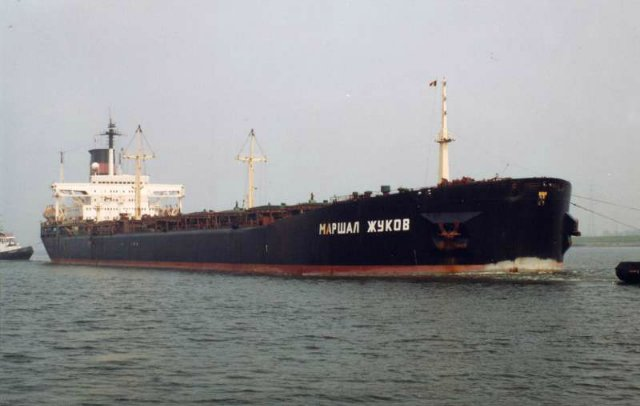
\includegraphics[scale=0.5]{Figs/marshl_jukov.jpg}
    \caption{Теплоход <<Маршал Жуков>>}
    \label{fig:jukov}
\end{figure}

И подобные явления, как оказалось, описывались и задолго до франклина. В своей <<естественной истории>> Плиний Старший говорит о похожем явлении \cite{Plinii}. Позднее <<мертвая вода>> была воспроизведена в лабораторных условиях исследователями из франции \cite{deadWater}. Запись эксперимента доступна на видеохостинге youtube \cite{deadWaterVideo}.


Математически описать возникновение внутренних волн можно записав уравнение для сил, которые действуют на выведенную из равновесия частицу жидкости(Рис. \ref{fig:Forces}):

\begin{equation}
    m_b \vec{a}_b = \vec{P} + \vec{G}
\end{equation}
где $\vec{P}=\rho_w \vec{g} S \cdot h$ это сила Архимеда, $\rho_w$ плотность жидкости того слоя на котором находится частица, $\vec{g}$ -- ускорение свободного падения, $S$ -- площадь стороны частицы, $h$  -- глубина. $\vec{G} = \rho_b \vec{g} S \cdot h$,  $\rho_b$ -- плотность частицы жидкости.

В проекции на вертикальную ось:

\begin{equation}
    \frac{d^2 \xi}{dt^2} = \frac{(\rho_w-\rho_b)}{\rho_b}\cdot g
\end{equation}

Тут $\xi$ будет обозначать отклонение от положения равновесия $z_0$, тогда очевидно что плотность воды вокруг частицы и плотность частицы будет равна в положении равновесия при $\xi=0$ $\rho_w(z_0)=\rho_b$ тогда уравнение можно переписать:

\begin{equation}
    \frac{d^2 \xi}{dt^2} = \frac{\rho_w(z_0+\xi)-\rho_b}{\rho_b}\cdot g
    \label{eq:beg}
\end{equation}

Введем переобозначение, $z=z_0+\xi$ тогда правая часть уравнения запишется $$\frac{\rho_w(z_0+\xi)-\rho_b}{\rho_b}\cdot g = \frac{\rho_w(z)-\rho_w(z_0)}{\rho_w(z_0)}\cdot g = \frac{1}{\rho(z_0)} \frac{\rho_w(z)-\rho_w(z_0)}{z-z_0}\cdot(z-z_0) g$$

При достаточно малом $t$ отклонении от положения равновесия $z$ будет также мало, что дает нам возможность перейти к производной по $z$, а $\rho_w$ переобозначим как $\rho$ и окончательно запишем:

\begin{equation}
    \frac{d^2 \xi}{dt^2} =\frac{1}{\rho} \frac{d\rho}{z}\xi \cdot g
\end{equation}

Решение этого дифференциального уравнения ищется в виде периодической функции, это значит, что частица совершает колебания около своего положения равновесия:

\begin{equation}
    \xi(t)=A cos(\omega t + \phi)
\end{equation}

подставим выражения $\xi(t)$ в уравнение:

\begin{equation}
    \ddot{\xi} = - A \omega^2 cos(\omega t + \phi )
\end{equation}

или если выразить правую часть через $\xi$

\begin{equation}
    \ddot{\xi} = - \omega^2  \xi
    \label{eq:final}
\end{equation}

Подставим (\ref{eq:final}) в (\ref{eq:beg}):

\begin{equation}
    -\omega^2 \xi = \frac{1}{\rho_0}\cdot \frac{d \rho}{d z} \xi g
\end{equation}

Выразим частоту колебаний частицы:

\begin{equation}
    \omega(z) = N(z) = \sqrt{- \frac{g}{\rho_0}\cdot\frac{d \rho(z)}{dz}}
\end{equation}

Эта частота называется частота плавучести или Частота Брента — Вяйсяля. В океане она составляет величину порядка $10^{-3}$ $\frac{1}{\textup{с}}$ \cite{King2012}.

\begin{figure}
    \centering
    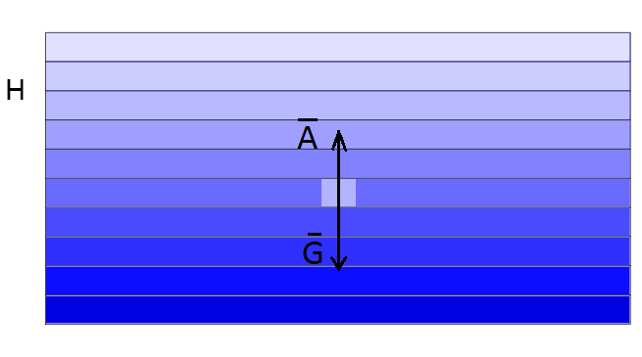
\includegraphics[scale=0.8]{Figs/Forces.png}
    \caption{Схематичное представление сил действующие на частицу выведенную из равновесия в стратифицированной жидкости, цветом показана плотность.}
    \label{fig:Forces}
\end{figure}

\begin{figure}
    \centering
    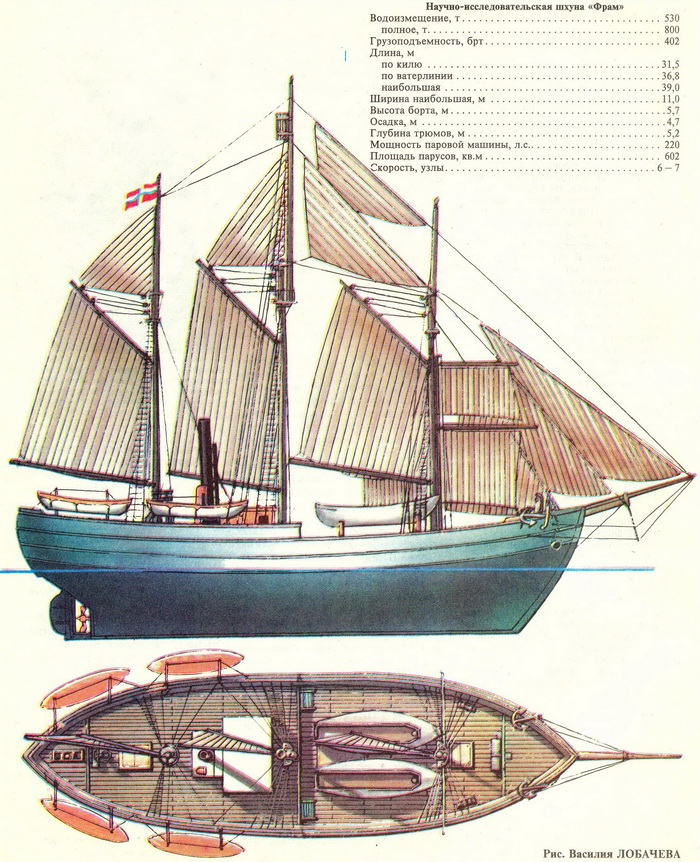
\includegraphics[width=1\textwidth]{Figs/FRAM.jpg}
    \caption{Исследовательское судно <<Фрам>>}
    \label{fig:fram}
\end{figure}

\begin{figure}
    \centering
    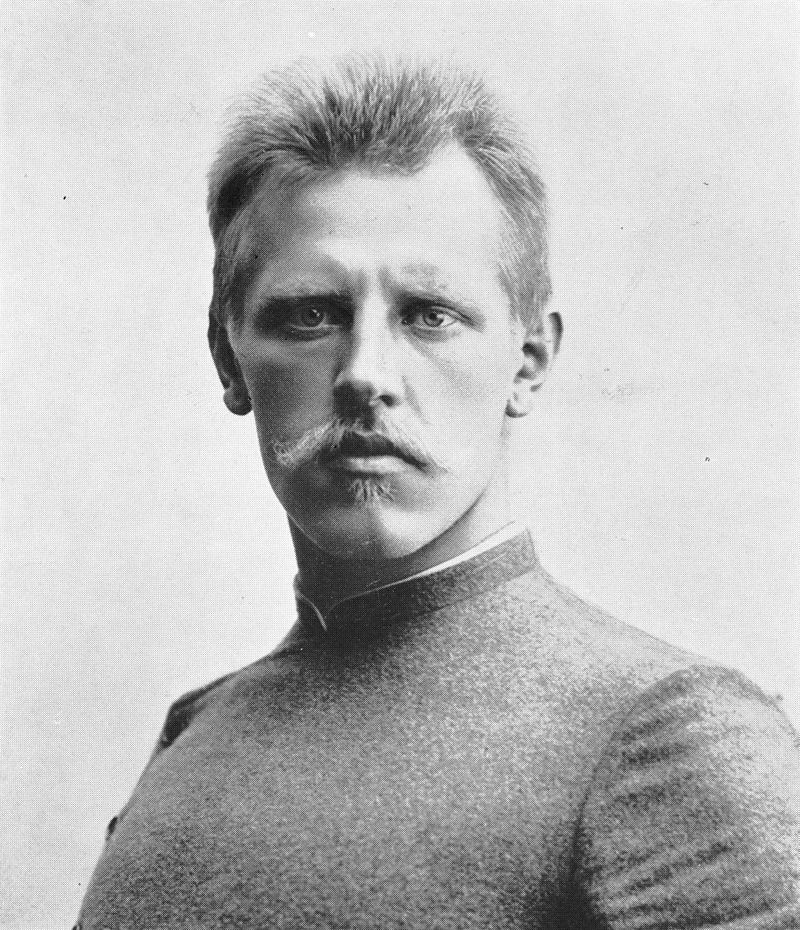
\includegraphics[scale=2.5]{Figs/800px-Fridtjof_Nansen.jpg}
    \caption{Фритьоф Ведель-Ярлсберг Нансен (1861-1930)}
    \label{fig:Nansen}
\end{figure}

\section{Обзор литературы}

Внутренние волны очень распространенное явление в океане. Существуют они благодаря перепадам плотности на разной глубине, сила плавучести играет роль восстанавливающей силы. Океаны являются одним из естественных примеров стратифицированных сред. Основные источники внутренних волн в океане это приливные эффекты, которые сопряжены с движением Земли относительно Солнца и Луны относительно Земли.

Внутренние волны активно взаимодействуют с другими океаническими структурами \cite{Rainville2006} и с неровностями океанического дна \cite{DAUXOIS1999}. Процессы перемещения внутренних волн их взаимодействия друг с другом и океаническими структурами различных масштабов образуют собой явление называемое энергетическим каскадом\cite{Garrett1972}. Энергетический каскад способствует поддержанию глобальной океанической циркуляции и перемешиванию\cite{Nikurashin2012,Munk1998}. Тем не менее, механизмы вносящие крупномасштабный приливный вклад в движение внутренних волн недостаточно понятны \cite{Ivey2008,Polzin1997} и каскадный процесс остается одной из фундаментальных проблем современной океанографии. Главным образом остаются вопросы связи крупномасштабных и мелкомасштабных явлений.

Одним из объяснений этой связи могут послужить аттракторы внутренних гравитационных волн. Это явление, при котором внутренние волны многократно отражаясь от поверхности океана, его дна и неровностей движутся по замкнутым орбитам. Возникновение такого явление возможно лишь в том случае, когда на дне океана имеются определенные комбинации геометрических неровностей. Аттракторы передают кинетическую энергию крупномасштабных эффектов, такие как приливы и внутренние волны большой длинны к мелкомасштабным явлениям волновой турбулентности и перемешиванию. Происходит это благодаря явлению фокусировки, в результате которого длинна внутренних волн уменьшается, но увеличивается амплитуда.

Возможность возникновения аттракторов в океане с реальной геометрией дна уже исследовалась\cite{Tang2010}. Например, топология северной части хребта Лусона имеет соответствующую геометрию. Эксперименты~\cite{ECHEVERRI2011} подтверждают возможность образования аттракторов внутренних волн. Кроме того при моделировании внутренних волн в условиях случайного разреза геометрии океанического дна, был сделан вывод, что с немалой вероятностью возможны возникновения аттракторов по одному на каждую сотню километров океанического дна \cite{Guo2015}. Тем не менее стоит отметить, что на данный момент нет свидетельств наблюдаемых волновых аттракторов. Возможно это связано с тем, что теоретические работы\cite{Guo2015} относятся к двумерному океану, но также существуют трехмерные конфигурации геометрий в которых возможны существования трехмерных волновых аттракторов\cite{Drijfhout2007,Manders2004}. Кроме того, в теоретическом представлении аттракторов внутренних волн не учитывается шероховатость поверхностей отражения. Однако надежность теоретических соображений о возможности существования трехмерных аттракторов была экспериментально проверена\cite{Hazewinkel2010}. Кроме того волновые явления в океане часто имеют целый спектр частот\cite{Garrett1972}, в то время как многочисленные эксперименты проводятся лишь с монохроматическим источником внутренних волн.

Предполагается, что аттракторы могут влиять не только на перемешивание, но и на движение мелких животных, явление седиментации и эрозию прибрежных конструкций.

Работы по фокусировке внутренних волн и образованию устойчивых аттракторов ведутся с конца двадцатого века. Первое теоретическое предсказание аттракторов было сделано Лео Маасом в 1995 году\cite{Maas1995}. Через два года последовали экспериментальные исследования этого явления, теоретические результаты были воспроизведены\cite{Maas1997}. Эффекты фокусировки характерны не только для стратифицированной жидкости, но и для вращающихся \cite{articleMaas2003,Veronis1970}. В дальнейшем теоретические основы явления были пересмотрены на основании данных эксперимента\cite{Lam2008}.

Вместе с развитием вычислительной техники развивались и инструменты численного моделирования физических явлений. Во втором десятилетии двадцать первого века стало возможным численное моделирование трехмерных аттракторов внутренних волн. Первая удачная попытка была предпринята с использованием метода спектральных элементов\cite{Brouzet2016,Brouzet_2016}. При сравнении с экспериментом ошибка численного моделирования составила не больше 10\%. Также была предпринята попытка моделирования аттрактора внутренних волн с помощью метода конечного объема\cite{Brouzet2014}. Количественно воспроизвести результаты, полученные с помощью метода спектральных элементов не удалось.
Традиционно для моделирования аттракторов применяются уравнения Навье-Стокса в приближении Буссинеска. Однако существует ряд работ, где вместо классического подхода используется квазигидродинамический\cite{ElizarBook}. Квазигидродинамические уравнения позволяют добиться большей точности\cite{Kraposhin20182} при моделировании методом конечного объема.


\section{Математические модели для изучения внутренних гравитационных и инерционных волн}

Для описания движения несжимаемой жидкости используется уравнение Навье-Стокста. Но при небольшом перепаде плотности допустимо использовать уравнение Навье-Стокса в приближении Буссинеска, которое учитывает сжимаемость в члене с плавучестью.

\begin{equation}
 \large \frac{\partial \vec U}{\partial t} + (\vec U \cdot \nabla) \vec U = - \frac{1}{\rho_m} \nabla \hat p + \nu \Delta \vec U  + \vec f,
 \label{eq:momClassic}
\end{equation}
Уравнение переноса соли $s$:
\begin{equation}
 \large \frac{\partial \rho_s}{\partial t} + \vec U \cdot \nabla \rho_s  = \nabla \cdot \frac{\nu}{Sc} \left ( \nabla \rho_s \right ),
 \label{eq:transClassic}
\end{equation}
\begin{equation}
 \large \nabla \cdot \vec U  = 0.
 \label{eq:contClassic}
\end{equation}

Здесь $\vec{U}$ -- вестор скорости с компонентами $u_x,u_y; \nu$ -- кинематическая вязкость жидкости; $\rho_m$ -- значение плотности на верхней границе; $\rho_s$ -- добавка к плотности обусловленная наличием солености; приведенное давление $\hat{p}=p-p_0$, разница между полным и гидростатическим давлением; $\vec{f}=\frac{\rho_s}{\rho_m} \vec{g}$ -- восстанавливающая сила; Число Шмидта представляет собой отношение кинематической вязкости и коэффициента диффузии:  $Sc = \frac{\nu}{D}$. 

В данной работе помимо классических уравнений Навье-Стокса в приближении Буссинеска используются квазигидродинамические уравнения, работа над которыми ведется в институте прикладной математики имени Келдыша с восьмидесятых годов двадцатого века \cite{bookELIZ}. Различие между уравнениями Навье-Стокса несжимаемой жидкости и квазигидродинамическими уравнениями заключается в дополнительных диссипативных слагаемых. Эти слагаемые были первоначально введены для разреженного газа как способ сохранить инвариантность при пространственно-временном усреднении\cite{AIAAJ1995}. Физическая интерпретируемость в случае несжимаемой жидкости после обобщения теряется, но математически уравнения все еще верны \cite{Elizarova2011}. Как будет показано ниже диссипативные слагаемые могут быть весьма полезны при численном моделировании. 

Система приведенная ниже называется квазигидродинамической системой и впервые была получена Шеретовым \cite{ElSh2001}. Система является регуляризованным аналогом приближения Буссинеска, где $ \rho = const $.

 
Уравнение неразрывности дополняется добавочной скоростью $\vec{W}$:

    \begin{equation}
      \nabla \cdot \left (\vec U - \vec W \right ) = 0,
      \label{eq:cont}
    \end{equation}
уравнение импульса для квазигидродинамических уравнений:
\begin{equation}
      \frac{\partial \vec U}{\partial t} + \nabla \cdot \left ( (\vec U - \vec W)\otimes \vec U  \right )
      -
      \nabla \cdot \nu \left ( \nabla \vec U + (\nabla \vec U)^T \right ) - \nabla \cdot \left  (   \vec U \otimes \vec W \right )
      = 
      - \frac{1}{\rho} \nabla \Tilde{p} + \vec F,
\end{equation}
где $\nu$ - кинематическая вязкость; $\rho$ - плотность на верхней границе; $ \vec{F}$ - объемная сила; $\Tilde{p}$ давление без учета статического.

Дополнительную скорость можно записать как правую часть уравнения движения Эйлера:
\begin{equation}
      \vec W = \tau \left ( \vec U \cdot \nabla \vec U + \frac{1}{\rho} \nabla \Tilde{p} - \vec F  \right ),
      \label{eq:W}
\end{equation}

Массовая сила $\vec{F} = \beta g \Tilde{s}$ может определять поведение стратифицированной жидкости. $ \tau $ - параметр регуляризации. $ \beta $ - коэффициент соленостного сжатия $ \beta = \frac{1}{\rho}\frac{\partial \rho}{\partial s} $. В этом случае системе требуется дополнительное уравнение для отклонения начальной солености $ \Tilde{s} = s (x, y, z, t) - s (x, y, z, 0) $:

\begin{equation}
     \frac{\partial s }{\partial t} + \nabla \cdot \left ( (\vec U - \vec W) s \right )
      - \nabla \cdot \frac{\nu}{Sc} \left ( \nabla s \right ) - \nabla \cdot \left (\tau \vec{U} \cdot (\vec{U} \cdot \nabla s) \right) = 0,
\end{equation}
Уравнение для давления может быть получено напрямую путем подстановки выражения для дополнительной скорости в уравнение неразрывности \ref{eq:cont}:

\begin{equation}
     \nabla \cdot \frac{\tau}{\rho}\nabla \Tilde{p} = \nabla \cdot \left (   \vec{U} - \tau (\vec{U} \cdot \nabla \vec{U}) +  \tau \vec{F} \right ).
\end{equation}
Эти уравнение описывают движение соленой несжимаемой вязкой жидкости. Они могут быть сведены к классической системе уравнение если положить $\tau = 0$.

Для замыкания системы уравнений требуется задать граничные условия. Вход потока устанавливается как значение скорости, которое может зависеть от координат и времени по известному закону. Также необходимо определить градиент давления и солености:



\begin{equation}\label{eq:qhd_inlet}
    \vec{U} = \vec{U}_b, \,\,\, \frac{\partial \tilde p}{ \partial \vec{n}} = \rho_0 \vec n \cdot \left ( -\vec U_b \cdot \nabla \vec U + \vec F \right), \,\,\, s = s_b,
\end{equation}  

\begin{equation}\label{eq:qhd_outlet}
        \frac{\partial \vec{U}}{\partial \vec{n}} = 0, \,\,\, \tilde p = 0, \,\,\, \frac{\partial s}{ \partial \vec{n}} = 0,
\end{equation}

\begin{equation}\label{eq:qhd_walls}
        \vec{U} = 0, \,\,\, \frac{\partial \tilde p}{ \partial \vec{n}} = \rho_0 \vec n \cdot \left ( -\vec U_b \cdot \nabla \vec U + \vec F \right), \,\,\, \lambda \frac{\partial s}{ \partial \vec{n}} + \gamma s = \psi,
\end{equation}
Где $\vec U_b$ -- известное значение скорости на входе в поток,
$s_b$ -- известное значение солености на входе,
$\lambda$, $\gamma$ and $\psi$ -- специальные постоянные для переключения граничных условий между условием неймана и Дерихле скалярной величины $s$,
Граничные условия Неймана для давления определяются из следующего условия для регуляризованного потока:
$\vec n \cdot \vec W = 0$.


Таким образом описано два подхода к моделированию стратифицированной жидкости. Первый, классический представляет собой систему уравнений Навье-Стокса в приближении Буссинеска. Второй, регуляризованный представляет собой систему квазигидродинамических уравнений. 

\section{Линеаризованная теория внутренних гравитационных волн}

Ранее рассмотрена полная система уравнений, описывающая движение стратифицированной жидкости. Чтобы упростить задачу, можно предположить, что поток является двумерным и содержится в плоскости $xOz$ без изменений в направлении $y$. В этих рамках, используя уравнение неразрывности (\ref{eq:contClassic}), можно ввести функцию тока, определяемую как

\begin{equation}
    \frac{\partial \psi}{\partial x} = - u_z \;\;\;\;\;\;\;\; и \;\;\;\;\;\;\;\; \frac{\partial \psi}{\partial z} = - u_x
\end{equation}

тогда можно переписать уравнения (\ref{eq:momClassic}), (\ref{eq:transClassic}) и (\ref{eq:contClassic}) как

\begin{equation}
    \partial_{tz} \psi + J(\partial_z \psi, \psi) = - \frac{1}{\rho} \partial_x P + \nu \partial_z \Delta \psi,
    \label{eq:tokz}
\end{equation}

\begin{equation}
    \partial_{tx} \psi + J(\partial_x \psi, \psi) = \frac{\rho_s}{\rho_m}\vec{g}+\frac{1}{\rho}\partial_z P + \nu \partial_x \Delta \psi,
    \label{eq:tokx}
\end{equation}

\begin{equation}
    \partial_t \rho_s + J(\rho_s,\psi) = \nabla \cdot \frac{\nu}{Sc} (\nabla \rho_s) + \frac{d \rho}{dz} \partial_x \psi,
\end{equation}
где $J$ это яклбиан определенный как $J(f,g) = \partial_x f \partial_z g - \partial_z f \partial_x g.$ Обозначим как $\partial_j \psi =\frac{\partial \psi}{\partial j}$, где $j$ обозначает $x,y$ или $t$. 

В дальнейшем предполагается, что возмущения плотности $\rho_s(x; z; t)$ малы по сравнению с фоновой стратификацией $\rho(z)$. Это предположение полностью верно как в океане, так и экспериментах, рассматриваемых тут. Таким образом, возмущения плотности ограничиваются менее чем 10\% средней стратификации. 

Дифференцируя уравнение (\ref{eq:tokz}) по $z$, а (\ref{eq:tokx}) по $x$ и складывая их получаем

\begin{equation}
    \partial_t(\Delta \psi) + J (\Delta \psi, \psi) - \nu \Delta (\Delta \psi) = \frac{g}{\rho_m} \partial_x \rho_s,
    \label{eq:tokzz}
\end{equation}

\begin{equation}
    \partial_t \rho_s + J(\rho_s,\psi) - \nabla \cdot \frac{\nu}{Sc} (\nabla \rho_s) = -N^2 \frac{\rho_m}{g}\partial_x \psi.
    \label{eq:tokxx}
\end{equation}

Уравнения (\ref{eq:tokzz}) и (\ref{eq:tokxx}) описывают нелинейную динамику вязкой стратифицированной жидкости с диффузией. Уравнения для линейной динамики получаются путем пренебрежения нелинейными членами. Это приводит к

\begin{equation}
    \partial_t(\Delta \psi) + \nu \Delta (\Delta \psi) = \frac{g}{\rho_m} \partial_x \rho_s,
\end{equation}

\begin{equation}
    \partial_t \rho_s - \nabla \cdot \frac{\nu}{Sc} (\nabla \rho_s) = -N^2 \frac{\rho_m}{g}\partial_x \psi.
\end{equation}

Рассмотрим решение в виде плоской волны к линеаризованной системе: $\psi = \psi_0 exp(i\omega t - i \vec{k} \cdot \vec{r})$ и $\rho_s=\rho_m exp(i\omega t - i \vec{k}\cdot \vec{r})$. Волновой вектор $\vec{k}=k_x \vec{e}_x + k_z \vec{e}_z$ и его модуль $k$.

Линейная система может быть записана в матричном виде

\begin{equation}
    \left(\begin{array}{cc} -k^2(i\omega + \nu k^2) & i \frac{g}{\rho_m}k_x
    \\[15pt] iN^2 \frac{\rho_m}{g}kx & i\omega + \frac{\nu}{Sc} k^2 \end{array}\right)
    \left(\begin{array}{c}\psi \\[15pt] \rho_s\end{array}\right) = 
    \left(\begin{array}{c}0 \\[15pt] 0\end{array}\right).
\end{equation}

Можно найти нетривиальное решение этой системы

\begin{equation}
    k^2 \left( i\omega + \nu k^2 \right) \left(i \omega \frac{\nu}{Sc} k^2 \right) + N^2 k^2_x = 0.
\end{equation}

Если рассмотреть систему без диссипативных членов, убрать диффузию и теплопроводность то уравнение примет вид:

\begin{equation}
    \left(\frac{\omega}{N}\right)=\frac{k^2_x}{k^2} \;\;\;\;\;\;\;\; или \;\;\;\;\;\;\;\; \frac{\omega}{N}=\pm \frac{|k_x|}{k}.
\end{equation}

Это дисперсионное соотношение линейных внутренних волн в невязкой и недиффузионной жидкости. Его можно записать, используя угол $\theta$ между вертикальной осью $z$ и волновым вектором $\vec{k}$

\begin{equation}
    \frac{\omega}{N} = \pm sin \theta.
    \label{eq:dispersion}
\end{equation}

Это чисто геометрическое соотношение, которое показывает как распространяются волны в стратифицированной жидкости(Рис. \ref{fig:ermExp}). Угол распространения определяется только частотой плавучести и частотой вынужденных колебаний. Наконец, стоит отметить, что в дисперсионном соотношении отсутствует характерный масштаб длины. Таким образом, длина внутренних волн определяется граничными условиями, только источником волн.

\begin{figure}
    \centering
    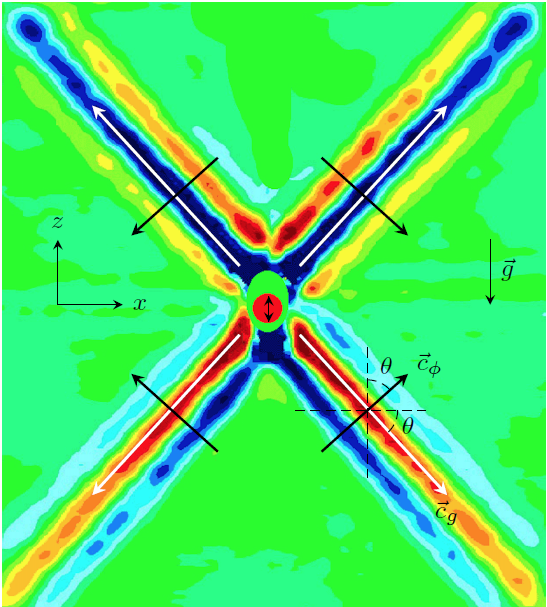
\includegraphics[scale=0.5]{Figs/Experement_Erm.png}
    \caption{Внутренние волны, излучаемые вертикально колеблющимся цилиндром, распространяются в линейно стратифицированной жидкости и  показаны красным в центре рисунка. Векторы групповой скорости показаны белым цветом, а векторы фазовой скорости - черным. Цветами обозначены поля горизонтального градиента плотности, полученные экспериментально Евгением Ерманюком с использованием методики SyS. Рисунок из \cite{brouzet:tel-01361201}}
    \label{fig:ermExp}
\end{figure}

%\subsection{Численные методы исследования волновых течений в неоднородных средах}


\section{Исследование свойств волновых течений с помощью трассировки лучей}

Дисперсионное соотношение дает мощный инструмент позволяющий качественно предсказать траекторию движения пучков внутренних волн, не только по удалению от источника но и при отражении от припятский(Рис. \ref{fig:internalReflection}). Поле отражения внутренняя волна сохраняет угол с вертикалью. Кроме того внутренние волны обладают ствойством фокусировки что выражается в сокращении расстояния между двумя параллельно пущенными лучами поле отражения от наклонной стенки. 

\begin{figure}
    \centering
    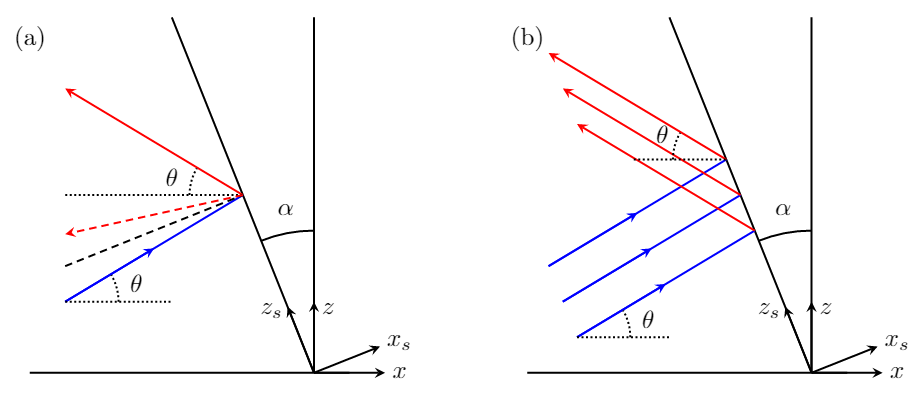
\includegraphics[scale=0.5]{Figs/angle_of_reflection.png}
    \caption{Отражение пучка внутренних волн от наклонной стенки. а) Отражение одного пучка, падающий волновой луч изображен синим цветом, отраженный от наклонной стенки красным, точками обозначена биссектрисса. Черным пунктиром обозначен перпендикуляр к наклонной поверхности, красным пунктиром луч отраженный <<зеркально>> по правилу Евклида. b) Отражение нескольких волновых лучшей от наклонной поверхности, отраженные лучи стали ближе, чем были падающие.}
    \label{fig:internalReflection}
\end{figure}

Трассировка лучей позволяет последовательно проследовать по траектории движения линейных внутренних волн без дисперсии и диффузии. В 1995 году Лео Маас обнаружил, что в трапециевидном резервуаре после множественных отражений внутренние волны зацикливаются около траектории которая имеет форму параллелограмма\cite{Maas1995}. Рис. \ref{fig:RayTr} показывает результат трассировки лучей в трапециевидном резервуаре.

\begin{figure}
    \centering
    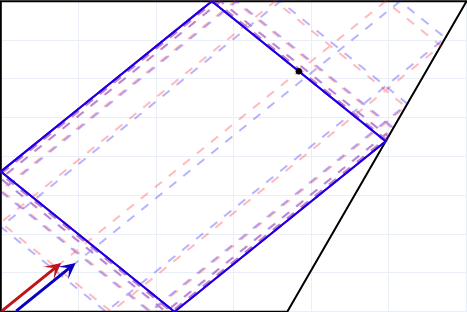
\includegraphics[scale=0.8]{Figs/RayTracing.png}
    \caption{Результат многократного отражения двух параллельных лучей внутренних волн}
    \label{fig:RayTr}
\end{figure}

Говоря о трассировки лучей нельзя не упомянуть о диаграмме Мааса\cite{Maas1997}. В задачах моделирования аттрактора имеется множество параметров:

\begin{itemize}
    \item Угол наклона стенки
    \item Частота плавучести
    \item Частота колебаний волнопродуктора
    \item Длинна резервуара
    \item Высота резервуара
\end{itemize}

Задачу трассировки лучей можно упростить, введя параметры. В своей работе он предлагает параметризовать резервуар фокусировки внутренних волн следующим образом(Рис. \ref{fig:domainTran}):

Применяется преобразование горизонтальной координаты, которое перемещает систему координат таким образом чтобы левый конец резервуара соответствовал координате $-1$ а правый $1$. Вводится параметр $d$ который обозначает расстояние от нуля новой горизонтальной оси до точки соприкосновения наклонной стенки с горизонтальной осью.
\begin{equation}
    x'=\frac{x\cdot 2}{L_1}-1
    \label{eq:transformX}
\end{equation}

Затем преобразование вертикальной координаты, которое сжимает или растягивает высоту резервуара так чтобы угол отражжения и распространения внутренних волн стал $45^\circ$. При этом вводится параметр $\tau$, который обозначает новую высоту резервуара. 
\begin{equation}
    z'=\frac{z\cdot 2}{L_1}\sqrt{\frac{N^2}{\omega^2}-1}
    \label{eq:transformZ}
\end{equation}

Таким образом вместо пяти определяющих параметров для геометрической задачи, остаются всего два, $d$ и $\tau$.

Благодаря методу трассировки лучей можно геометрически предсказать форму аттрактора внутренних волн. 

\begin{figure}
    \begin{subfigure}{\textwidth}
    \centering
    \begin{tikzpicture}[scale=0.7]
        \draw[thick] (0,0)--(0,4)node[left]{$H$}--(6,4)--(3.7,0)--(0,0);
        \draw[dashed] (6,4) -- (6,0)node[below]{$L_1$};
        \draw[thick,->] (6.2,2)->node[above]{$x'=\frac{x\cdot 2}{L_1}-1$}(14,2);
        \draw[->] (0,0)->(0,5)node[above]{$z$};
        \draw[->] (0,0)->(7.5,0)node[right]{$x$};
        \draw[->] (0,0)->(1.2,1);
        \draw[black] (0.5,0) arc [start angle=0, end angle=75, radius=0.25cm] node [right] {$\theta$};
        \draw[thick] (14.2,0)node[below]{$-1$}--(14.2,4)node[left]{$H$}--(20.2,4)--(17.9,0)node[below]{$d$}--(14.2,0);
        \draw[dashed] (20.2,4) -- (20.2,0)node[below]{$1$};
        \draw[->] (17.2,0)->(21.7,0)node[right]{$x'$};
        \draw[->] (17.2,0)->(17.2,5)node[above]{$z$};
        \draw[->] (14.2,0)->(15.4,1);
        \draw [black] (14.7,0) arc [start angle=0, end angle=75, radius=0.25cm] node [right] {$\theta$};
    \end{tikzpicture}
    \caption{Горизонтальное преобразование расчетной области}
    \end{subfigure}
    
    \begin{subfigure}{\textwidth}
    \centering
    \begin{tikzpicture}[scale=0.7]
        \draw[thick] (0,0)--(0,4)node[left]{$H$}--(6,4)--(3.7,0)--(0,0);
        \draw[dashed] (6,4) -- (6,0)node[below]{$L_1$};
        \draw[thick,->] (6.2,2)->node[above]{$z'=\frac{z\cdot 2}{L_1}\sqrt{\frac{N^2}{\omega^2}-1}$}(14,2);
        \draw[->] (0,0)->(0,5)node[above]{$z$};
        \draw[->] (0,0)->(7.5,0)node[right]{$x$};
        \draw[thick] (14.2,0)--(14.2,4.8)node[left]{$\tau$}--(20.2,4.8)--(17.9,0)--(14.2,0);
        \draw[black] (0.5,0) arc [start angle=0, end angle=75, radius=0.25cm] node [right] {$\theta$};
        \draw [black] (14.7,0) arc [start angle=0, end angle=80, radius=0.25cm] node [right] {$45^\circ$};
        \draw[->] (0,0)->(1.2,1);
        \draw[->] (14.2,0)->(15.4,1.2);
        \draw[dashed] (20.2,4.8) -- (20.2,0)node[below]{$L_1$};
        \draw[->] (17.2,0)->(21.7,0)node[right]{$x$};
        \draw[->] (14.2,0)->(14.2,6)node[above]{$z'$};
    \end{tikzpicture}
    \caption{Вертикальное преобразование расчетной области}
    \end{subfigure}
    \caption{Преобразования расчетной области для процедуры получения диаграммы Мааса}
    \label{fig:domainTran}
\end{figure}

На рисунке 

\begin{figure}
    \begin{subfigure}[с]{0.45\textwidth}
        \centering
        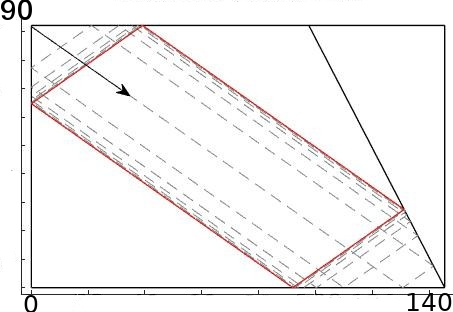
\includegraphics[scale=0.45]{Figs/RayTr923x1455.jpeg}
        \caption{Трассировка лучей,\\ $H=92.3$, $L=145.5$, $\theta = 35.13^{\circ}$,\\ $\alpha = 27.4^{\circ}$}
    \end{subfigure}
    \begin{subfigure}[r]{0.45\textwidth}
        \centering
        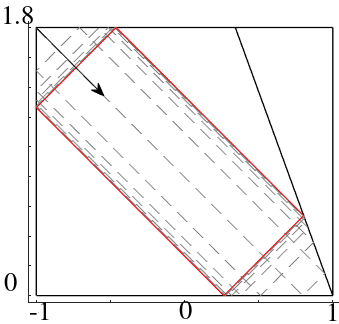
\includegraphics[scale=0.45]{Figs/RTdtau.png}
        \caption{Трассировка лучей в преобразованной геометрии, \\ $\tau = 1.8$, $d = 0.34$}
    \end{subfigure}
    
    
    \caption{Результат работы процедуры трассировки лучей и результат перехода к универсальным координатам $(d,\tau)$}


    \label{fig:RayTr923x1455}
\end{figure}

\chapter{Численное моделирование аттракторов внутренних гравитационных волн}
\label{cha:Simulation}

В данной главе рассматриваются три принципиально различных подхода к моделированию аттракторов внутренних волн.

Первый, метод спектральных элементов\cite{Patera1984}. Результаты полученные при помощи метода спектральных элементов были достаточно близки к результатам натурных экспериментов\cite{Brouzet2016,Brouzet_2016}. Недостатком метода является отсутсвие реализаций с открытым исходным кодом позволяющие встроить дополнительные физические модели и проводить расчеты на сложной геометрии приближенной к реальной топологии океанического дна.

Второй метод, метод конечных объемов на основе классических уравнений Навье-Стокса в приближении Буссинеска, качественно воспроизводит явление аттракторов, но количественно имеет большую погрешность. Однако его многочисленные реализации, в том числе и с открытым исходным кодом, предоставляют возможность для построения сложных сеток и геометрий. Также эти инструменты снабжены возможностями добавлять собственные реализации физических моделей, граничных условий и утилит. 

Третий способ также основан на методе конечного объема и сохраняет его преимущества, но он представляет собой реализацию квазигидродинамических уравнений\cite{ElizarBook}. Такой подход, еще называемый регуляризованным, обеспечивает точность выше, чем у реализации классической системы уравнений Навье-Стокса.

В работе рассматриваются различные конфигурации расчетной области (Рис. \ref{fig:dominleft},\ref{fig:domainup}).

\begin{figure}[!ht]
        \centering
          \begin{tikzpicture}[scale=1.0, z={(-.707,-.5)}]
            \draw (0,0,0) -- (6,0,0) -- (4,4,0)--(0,4,0) --cycle;
            \draw (0,0,0)     -- (6,0,0)   -- (4,4,0)   -- (0,4,0)    -- cycle;
            \draw[style = dashed] (2.7,4,0)   -- (0,1.8,0) -- (2.2,0,0) -- (5,2.1,0)-- cycle;
            %\draw[style = dashed] (0,0.985,0) -- (3.3,4,0) -- (4.5,3,0) -- (1.1,0,0)  -- cycle;

            \draw[<->] (-0.1,0) --node[above,rotate=90] {$H = 40$ cm} (-0.1,4);
            \draw[<->] (0,-0.1,0) --node[below,] {$L_2 = 60$ cm} (6,-0.1,0);
            \draw[<->] (0,4.1,0) --node[above,] {$L_1 = 40$ cm} (4,4.1,0);

            \draw[color=red] (3.0,0)--(3.0,4.0);
            
            \draw (3.15,0) node[above] {$A$};
            \draw (3.15,4.0) node[below] {$B$};

            \draw[thick,->] (4.95,3.5,0) -- (5.95,3.5,0) node[anchor=north east]{$x$};
            \draw[thick,->] (4.95,3.5,0) -- (4.95,4.5,0) node[anchor=north west]{$z$};
            \draw[thick,->] (5.3,3,0) -- (5.3,2,0) node[anchor=west]{$\vec{g}$};
          \end{tikzpicture}
          \caption{Вычислительная область для аттракторов внутренних волн, красным показана линия пробы, пунктиром показана предполагаемая форма аттрактора}
          \label{fig:dominleft}
\end{figure}

\begin{figure}[!ht]
    \centering
    \begin{tikzpicture}[scale=1, z={(-.707,-.5)}]
    \draw (3.6,0,0) -- (0,0,0) -- (0,4,0)--(6,4,0)--(3.6,0,0);
    %\draw (3.6,0,0) -- (3.6,0,-1) -- (6,4,-1) -- (6,4,0) -- cycle;
    %\draw (6,4,0) -- (0,4,0) -- (0,4,-1) -- (6,4,-1);
    \draw (-0.5,2,0) node{};
    \draw (4.1,-.2,-1.5) node{};
    \draw (3.5,5,0) node{};
    \draw[<->] (-0.1,0) --node[above,rotate=90] {$H = 40$cm} (-0.1,4);
    \draw[<->] (0,4.1,0) --node[above,] {$L_1 = 60$ cm} (6,4.1,0);
    \draw[<->] (0,-0.1,0) --node[below,] {$L_2=36.9$ cm} (3.6,-0.1,0);
    \draw [black, thick] (5.5,4) arc [start angle=180, end angle=240, radius=0.5cm]
        node [left] {$60^\circ$};
    \draw[thick,->] (5.5,1,0) -- (6.5,1,0) node[anchor=north east]{$x$};
    \draw[thick,->] (5.5,1,0) -- (5.5,2,0) node[anchor=north west]{$z$};
    \draw[thick,->] (3,3,0) -- (3,1,0) node[anchor=west]{$\vec{g}$};
    \end{tikzpicture}
    \caption{Конфигурация вычислительной области для аттрактора внутренних гравитационных волн}
    \label{fig:domainup}
\end{figure}

Принципиальной разницы в этих двух вариантах нет в первом случае волнопродуктор располагается на левой стенке, а во втором сверху.


\section{Численное моделирование аттракторов внутренних волн с помощью метода спектральных элементов}

Используемая реализация -- пакет с открытым исходным кодом nek5000\cite{NEK5000}. 

В методе спектральных элементов решение и данные представлены в виде полиномов тензорного произведения $N$-го порядка внутри каждого из $E$ деформируемых шестигранных (кирпичных) элементов. Типичные дискретизации включают $E = 100 - 10 000$ элементов порядка $N = 8 - 16$ (что соответствует $512 - 4096$ точкам на элемент). Векторизация и эффективность кеширования проистекают из локального лексикографического упорядочения в каждом макроэлементе и из того факта, что действие дискретных операторов, которые номинально имеют $O(E\cdot N \cdot 6)$ ненулевых значений, может быть оценено только за $O(E\cdot N \cdot 4)$ и $O(E\cdot N\cdot 3)$. хранение за счет использования факторизации тензор-произведение-сумма. Метод спектральных элементов демонстрирует очень небольшую числовую дисперсию и диссипацию, что может быть важно, например, при расчетах устойчивости, для длительного интегрирования и для потоков с большим числом Рейнольдса.

Nek5000 решает нестационарные несжимаемые двумерные, осесимметричные или трехмерные уравнения Стокса или Навье-Стокса с вынужденной или естественной конвекцией теплопередачи как в стационарной (фиксированной), так и в движущейся геометрии. Он также решает уравнение Навье-Стокса для сжимаемой жидкости при низких числах Маха.

На данный момент это самый точный способ численно воспроизвести эксперементальные данные\cite{Brouzet2016,Brouzet_2016}. Недостаток реализации заключается в том, что геометрия задается путем аффинных преобразований. Подобрать преобразование, которое отображало бы прямоугольник в сложную геометрию океанического дна представляется трудоемкой задачей. 

Для моделирования методом спектральных элементов используется конфигурация расчетной области представленная на рисунке \ref{fig:domainup}. На протяжении всего эксперимента на верхней стенки задается граничное условие для скорости:

\begin{equation}
    U_z = A\cdot cos\left(\frac{\pi \cdot z}{L_1}\right)\cdot \omega \cdot  sin(\omega_0 t)
\end{equation}

Где $\omega_0$ -- частота волнопродуктора. 

На остальных стенках для скорости:

\begin{equation}
    \vec{U} = 0
\end{equation}

Граничные условия для давления на стенках:

\begin{equation}
    \nabla p = 0
\end{equation}

Условие для градиента солености на стенках:

\begin{equation}
    \frac{\partial s}{\partial n} = grad(s_0)
\end{equation}

$s_0$ -- начальное распределение солености в резервуаре.

\begin{figure}[!ht]
    \centering
    \begin{subfigure}[с]{0.45\textwidth}
        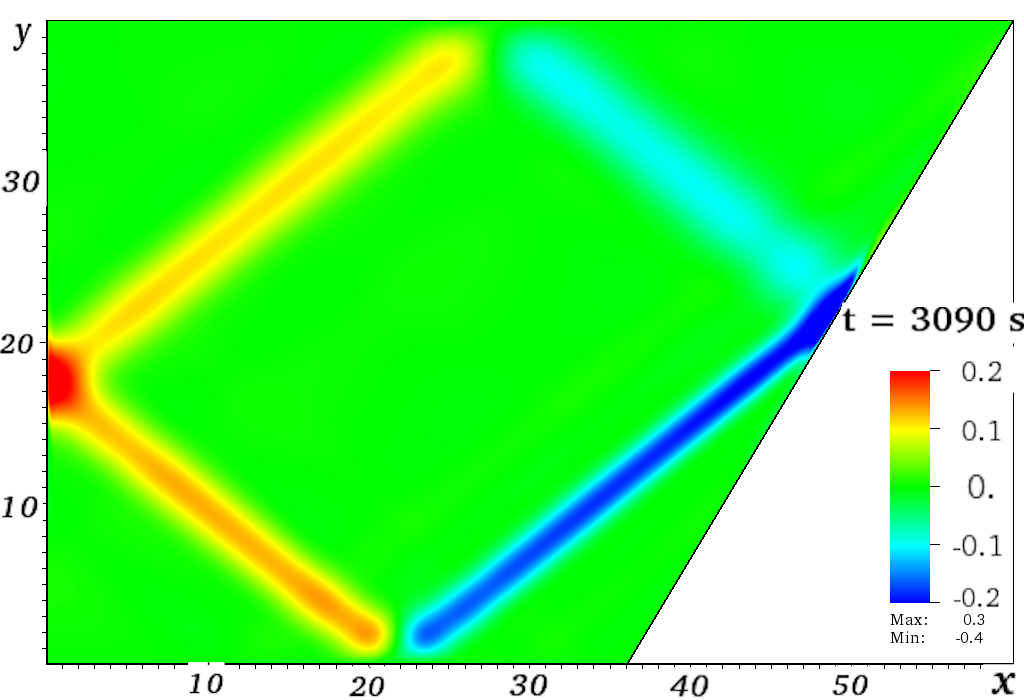
\includegraphics[scale=0.15]{pics/H40L60N1ap02dp20w0p63/2D36x36DiagramH40L60N1ap02dp20w0p63Vyn06179.png}
        \caption{Горизонтальная компонента скорости}
    \end{subfigure}
    \begin{subfigure}[с]{0.45\textwidth}
        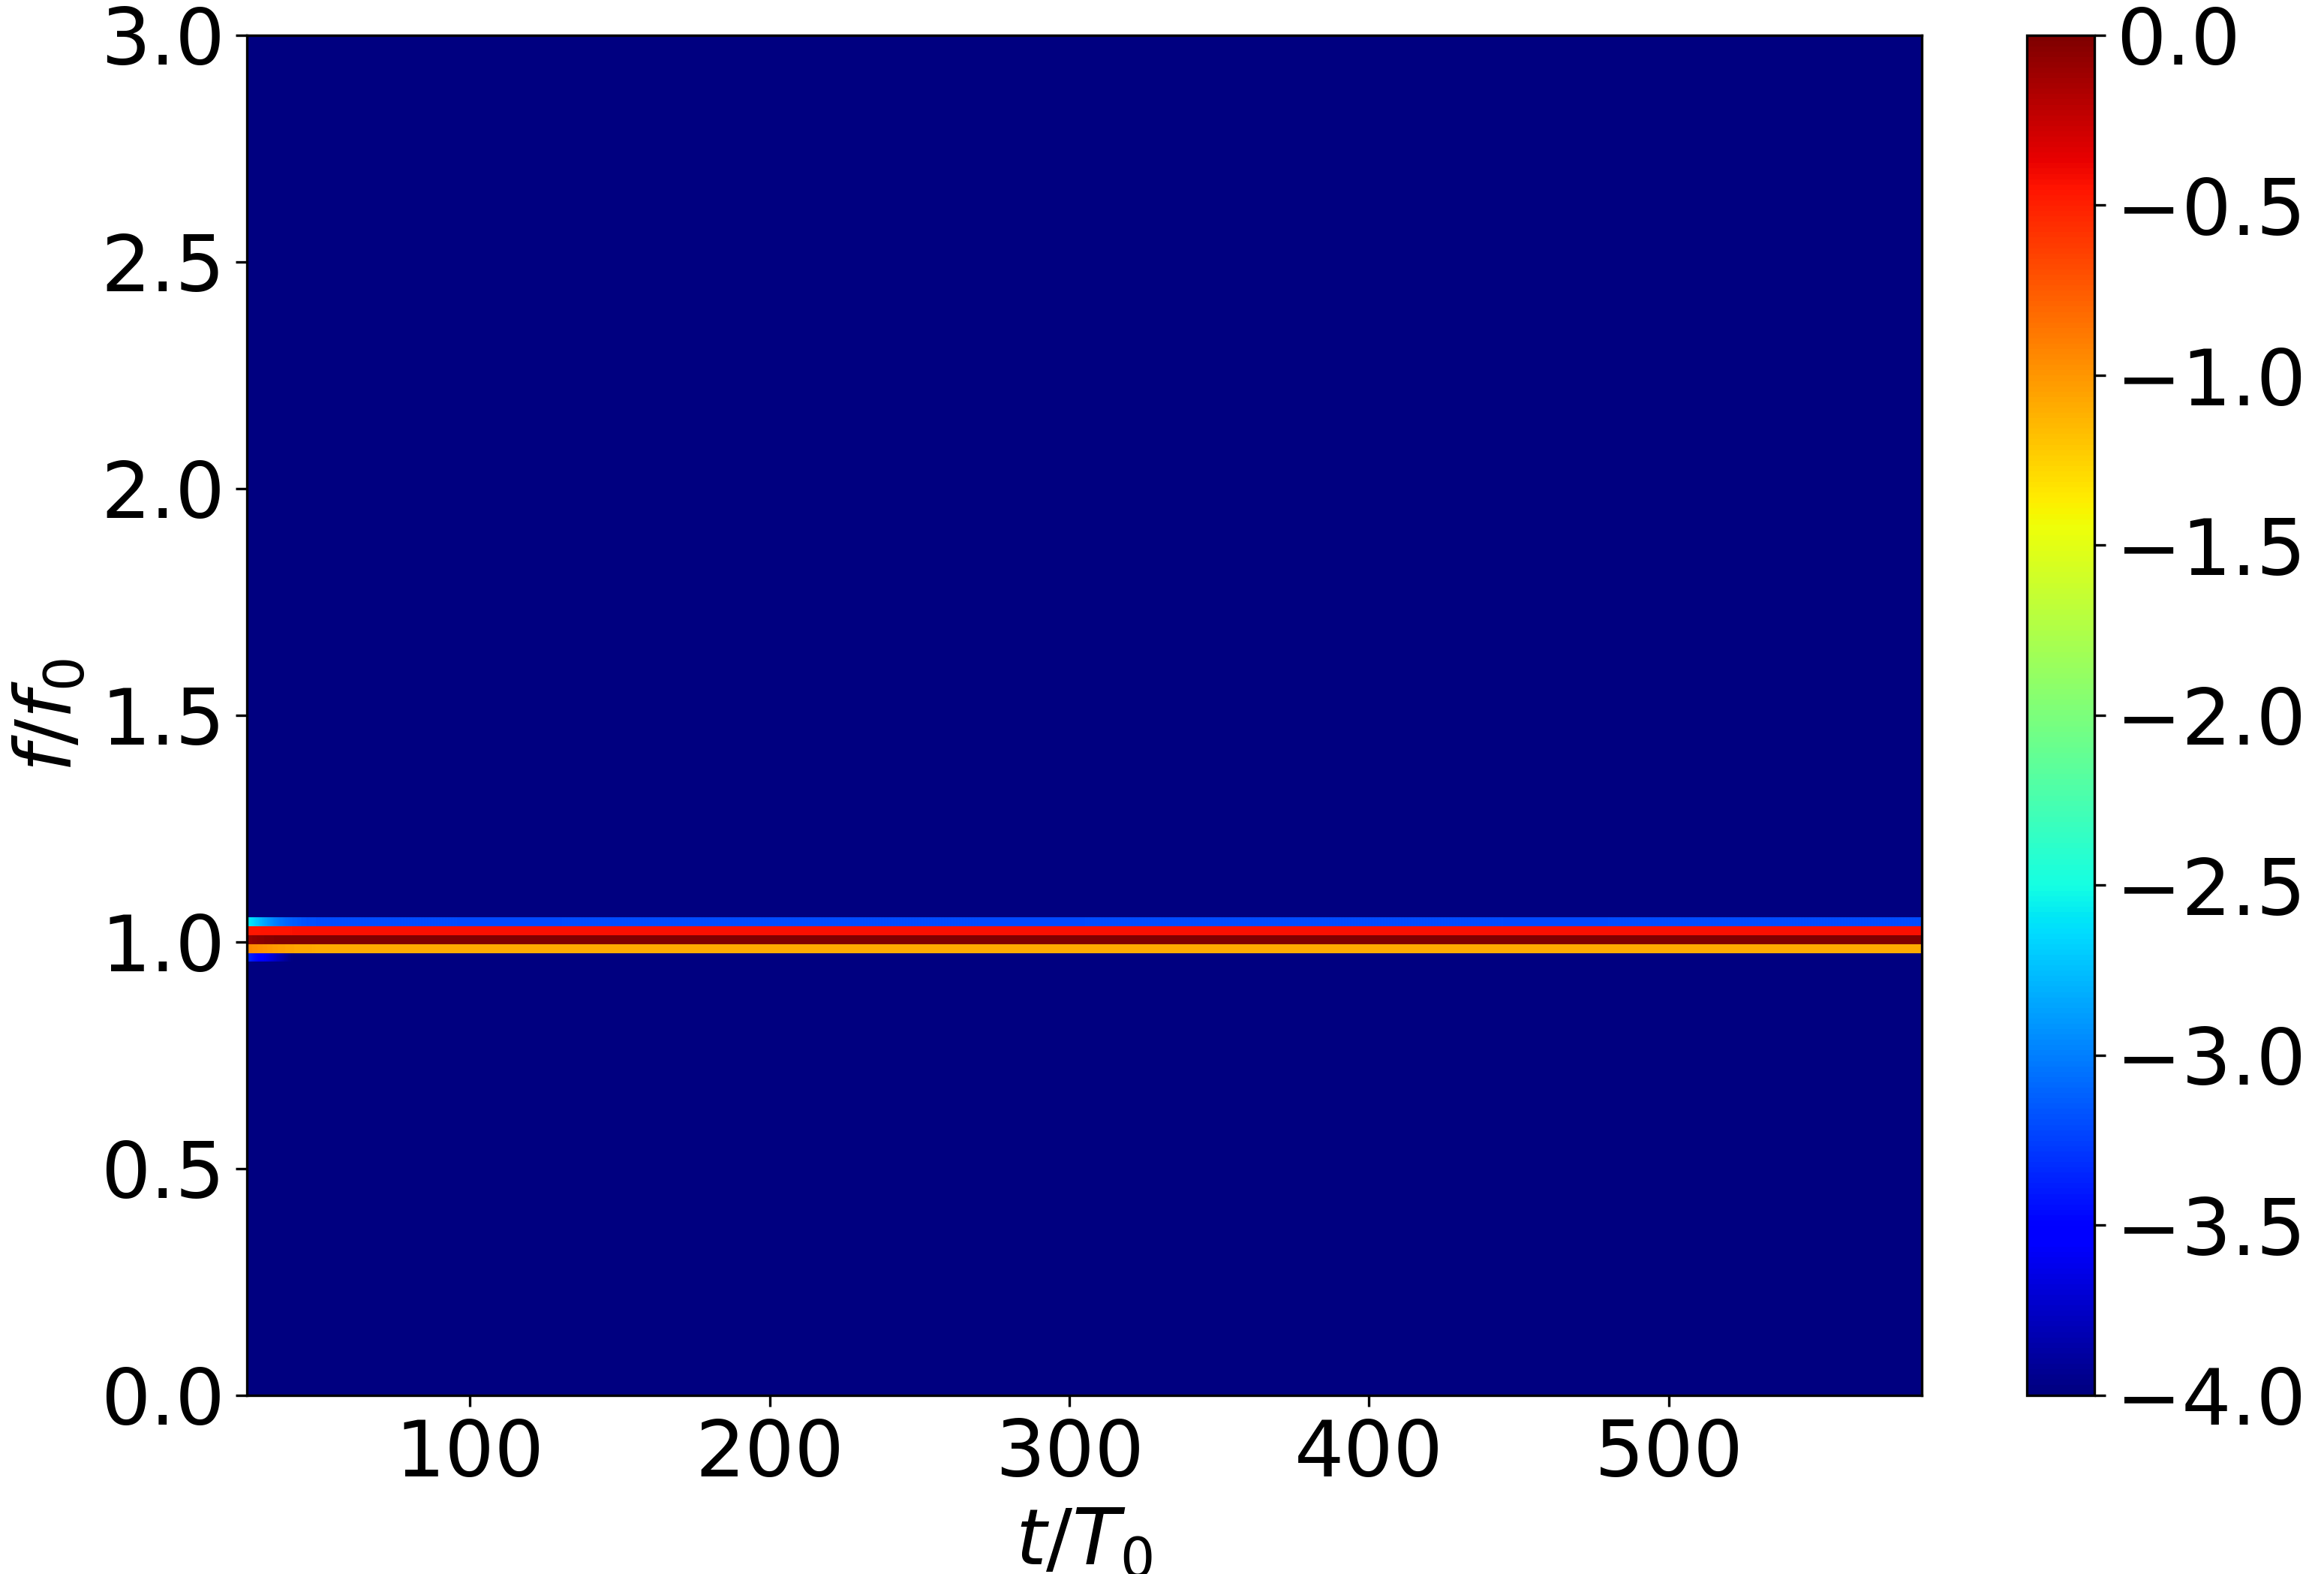
\includegraphics[scale=0.07]{pics/H40L60N1ap02dp20w0p63/TFspectrumX356Y112N1024.png}
        \caption{Частотно-временная диаграмма на аттракторе}
    \end{subfigure}
    \begin{subfigure}[с]{0.45\textwidth}
        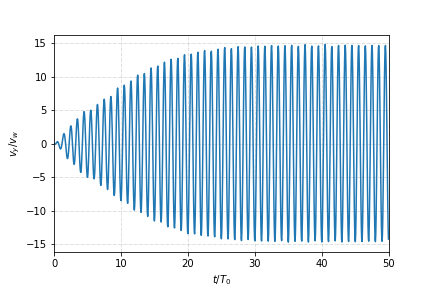
\includegraphics[scale=0.5]{pics/H40L60N1ap02dp20w0p63/vyX355662118341Y112748618745t1000.png}
        \caption{Амплитуда скорости в зависимости от времени на аттракторе}
    \end{subfigure}
    \begin{subfigure}[с]{0.45\textwidth}
        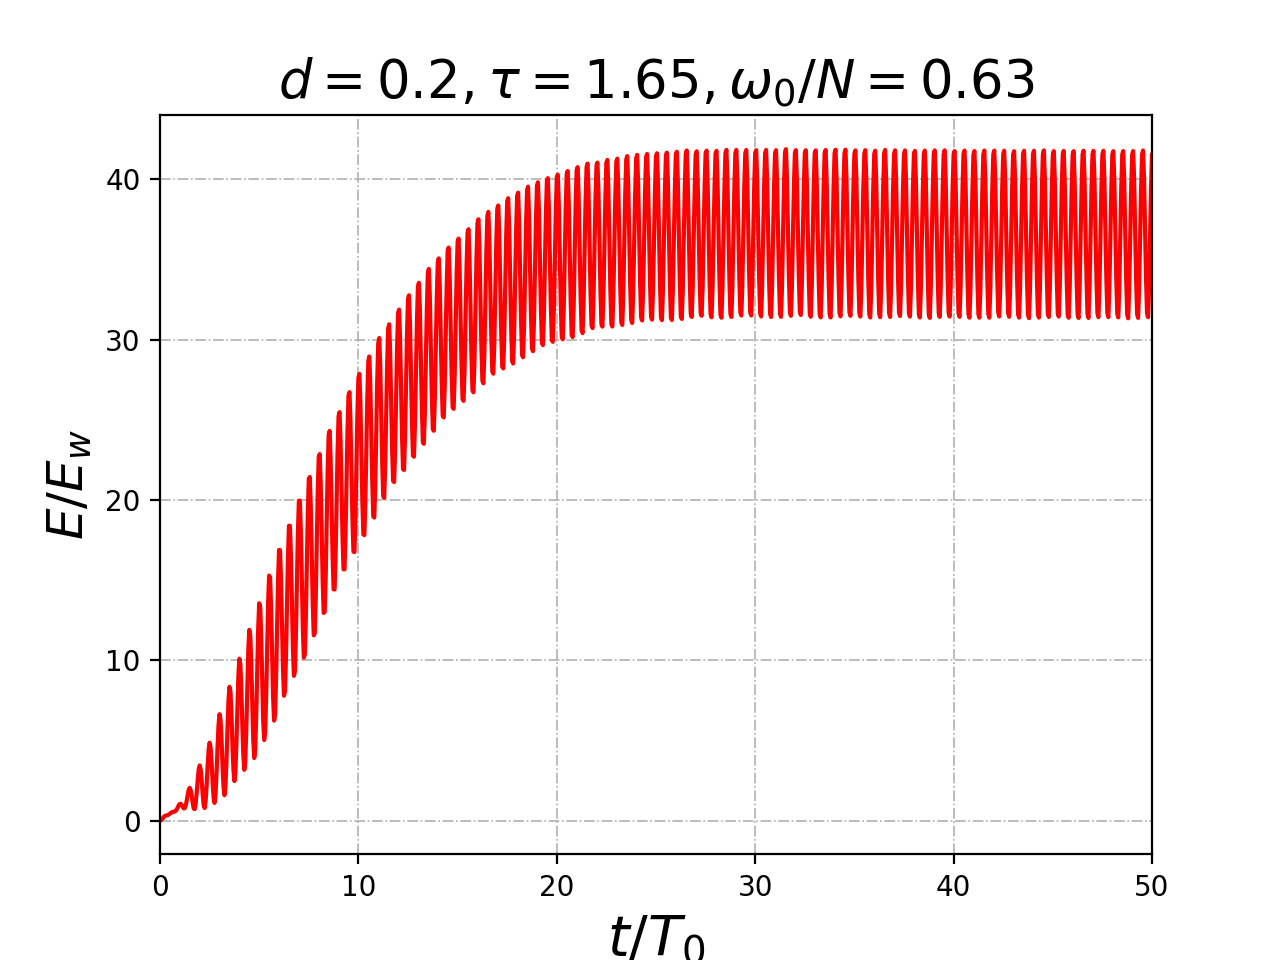
\includegraphics[scale=0.4]{pics/H40L60N1ap02dp20w0p63/2D36x36DiagramH40L60N1ap02dp20w0p63totKEnonDim.png}
        \caption{Средняя кинетическая энергия в резервуаре}
    \end{subfigure}
    
    \caption{Результат моделирования аттрактора внутренних волн методом спектральных элементов}

\end{figure}

В заключении можно сказать, что алгоритм высокого порядка точности хорошо воспроизводит результаты натурного эксперимента. В дальнейшем они будут использоваться как эталон для сравнения с остальными методами решения. 

\section{Численное моделирование аттракторов внутренних волн с помощью метода контрольного объема}

Для моделирование методом конечного объема используется конфигурация представленная на рисунке \ref{fig:dominleft} в этом случае волнопродуктор установлен на левой стенке и колеблется по следующему правилу:

\begin{equation}
    U_x = A\cdot cos\left(\frac{\pi \cdot z}{H}\right)\cdot \omega \cdot  sin(\omega_0 t)
\end{equation}

Аналогично условия на остальных стенках:

\begin{equation}
    \vec{U} = 0
\end{equation}

Для далвения:

\begin{equation}
    \nabla p = 0
\end{equation}

Для градиента солености:

\begin{equation}
    \frac{\partial s}{\partial n} = grad(s_0)
\end{equation}

В качестве алгоритма нахождения численного решения используется PISO \cite{IssaGosmanWatkins-PISO}. Вкратце изложить алгоритм нахождения полей скорости и давления можно так:
\begin{enumerate}[1.]
    \item Устанавливаются граничные условия.
    \item Решается дискредитированное уравнение движения для вычисления промежуточных значений поля скорости.
    \item Вычисляются массовые потоки через границы ячеек.
    \item Решается уравнение для давления.
    \item Корректируются массовые потоки.
    \item Корректируется поле скорости согласно новому давлению.
    \item Обновляются граничные условия.
    \item Вернуться к третьему шагу.
    \item Перейти на следующий временной шаг и начать с первого пункта.
\end{enumerate}
Внутри шага по времени тут имеется цикл между пунктом 3 и пунктом 8. Более того возможны коррекции неортогональности ячеек сетки если зациклить этот алгоритм между пунктом 4 и 5. дискредитированное уравнение движение в матричном виде можно записать следующим образом: 

\begin{equation}
    \mathcal{M} \vec{U}^* = -\frac{\nabla p}{\rho_m} + \vec{F}
\end{equation}
где $\mathcal{M}$ -- матрица коэффициентов, $\vec{U}^*$ -- искомые промежуточные значения поля скоростей. Для получения уравнения давления эта мтарица коэффициентов расщепляется следующим образом:

\begin{equation}
    \mathcal{M} \vec{U}^* = \mathcal{A} \vec{U}^* - \mathcal{\vec{H}}
\end{equation}
где $\mathcal{\vec{H}}$ -- источниковые члены для уравнения давления. $\mathcal{A}=diag(\mathcal{M})$. Подставляем расщепленную матрицу коэффициентов в уравнение движение:
\begin{equation}
    \mathcal{A} \vec{U}^* - \mathcal{\vec{H}}= -\frac{\nabla p}{\rho_m} + \vec{F}    
\end{equation}
Умножаем обе части на $\mathcal{A}^{-1}$, выражаем $\vec U$

\begin{equation}
    \mathcal{A}^{-1} \mathcal{A} \vec{U} = \mathcal{A}^{-1} \mathcal{\vec{H}} - \mathcal{A}^{-1} \nabla p + \mathcal{A}^{-1} \vec{F} \;\;=>\;\;
    \vec{U} = \mathcal{A}^{-1} \mathcal{\vec{H}} - \mathcal{A}^{-1} \nabla p + \mathcal{A}^{-1} \vec{F}
\end{equation}
согласно уравнению неразрывности $\nabla \vec{U} = 0$, это дает нам уравнение для давления:

\begin{equation}
    \nabla \cdot (\mathcal{A}^{-1} \nabla p) = \nabla \cdot (\mathcal{A}^{-1} \mathcal{\vec{H}} + \mathcal{A}^{-1} \vec{F})
\end{equation}

Алгоритм PISO не прост в понимании и сложен из-за двух вложенных циклов внутри одного временного шага. Но очень популярен и долгое время остается одним из самых востребованных инструментов вычислительное гидродинамики.

К сожалению, результаты моделирования аттрактора внутренних волн алгоритмом PISO количественно не соответствуют результатам полученным при помощи метода спектральных элементов. 

Подведя итог можно сказать следующее, популярный алгоритм качественно воспроизводит картину течения, образующуюся при многократном отражении внутренних волн от стенок трапециевидного резервуара. Но количественно нет. Преимуществом алгоритма является способность работать с неортогональными сетками и сложной геометрией. К недостаткам можно отнести сложность и нелинейность процедуры нахождения гидродинамических полей.

\begin{figure}[!ht]
    \centering
        \begin{tikzpicture}[scale=5.34, z={(-.707,-.5)}]
          \node[anchor=south west,inner sep=0] at (0,0) {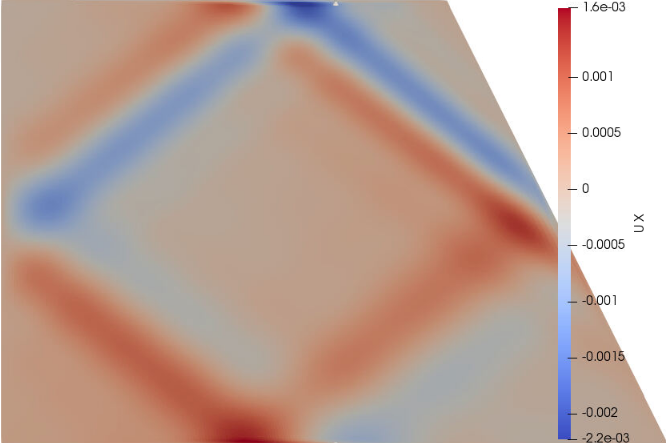
\includegraphics[width=\textwidth]{Figs/Attr200s.png}};
          \draw[thick,style = dashed] (1.5, 0, 0) -- (1.5, 2, 0);
        \end{tikzpicture}
    \caption{Поле горизонтальной компоненты скорости, пунктиром показана линия пробы}
    \label{fig:attractorRes}
\end{figure}



\begin{figure}[!ht]
    \centering
            \begin{tikzpicture}[scale = 1.1]
            \begin{axis}
                [scale only axis, grid=major,legend style={at={(0,1),font=\LARGE},anchor=north west}, ymin=-0.8*10^-3, ymax=1.7*10^-3,legend style={nodes={scale=0.5, transform shape}}, x post scale=1.6]

                \addplot[solid,color=red,thick] table [x=Points:1, y=Result, col sep=comma] {CSV/snappy180x180nCor4NonOrth4.csv};

                \addplot[solid,color=blue,thick] table [x=Points:1, y=Result, col sep=comma] {CSV/FVMnocor.csv};

                \addplot[solid,color=orange,thick,dashed] table [x=Points:1, y=Result, col sep=comma] {CSV/FVM450x2.csv};

                \legend{PISO 225x150*, PISO 225x150, PISO 450x300}
            \end{axis}
            \begin{axis}
                [scale only axis, ymin=-0.8*10^-1, ymax=1.7*10^-1, yticklabels={,,},xticklabels={,,},legend style={at={(0,0.76),font=\LARGE},anchor=north west},legend style={nodes={scale=0.5, transform shape}},x post scale=1.6]
%                \addplot[solid,thick] table [x=Points:1, y=x_velocity, col sep=comma] {CSV/Ux30Nek500T200.csv};
                \legend{NEK5000}
            \end{axis}
        \end{tikzpicture} 
    \caption{Результат моделирования с помощью агоритма PISO}
    \label{fig:PISOattr}
\end{figure}

\section{Численное моделирование аттракторов внутренних волн с помощью метода контрольного объема на базе квазигидродинамического подхода}

В этом разделе будут подробно разобраны способы аппроксимации слагаемых в квазигидродинамических уравнениях. Рассматриваются способы дискретизации уравнений и их реализация при помощи пакета с открытым исходным кодом OpenFOAM версии 1912\cite{OpenFOAM}.

OpenFOAM -- математический пакет с открытым исходным кодом. Аббревиатура FOAM означает Field Operation And Manipulation, то есть операции и манипуляции с полями. В OpenFAOM реализованные гибкие и современные инструменты как численного моделирования, так и разработки согласно современным стандартам языка С++ и объектно-ориентированного программирования. 

Для начала рассмотрим дискретные аналоги квазигидродинамических уравнений. Производные по времени аппроксимируются разностями согласно схеме Эейлера:

\begin{equation}
    \frac{\partial \vec{U}}{\partial t} \approx \frac{ \vec{U}_n-\vec{U}_o}{\Delta t}, \,\,\,
    \frac{\partial \Tilde{s}}{\partial t} \approx \frac{ \Tilde{s}_n-\Tilde{s}_o}{\Delta t},
\end{equation}
или с помощью схемы Адамса-Башфорта:

\begin{equation}
    \frac{\partial \vec{U}}{\partial t} \approx   \frac{1}{\Delta t} \left  (\frac{3}{2}\vec{U}_n - 2\vec{U}_o + \frac{1}{2} \vec{U}_{oo} \right), \,\,\,
    \frac{\partial \Tilde{s}}{\partial t} \approx \frac{1}{\Delta t} \left (\frac{3}{2}\Tilde{s}_n - 2\Tilde{s}_o + \frac{1}{2} \Tilde{s}_{oo}\right).
\end{equation}

Пространственная аппроксимация имеет второй порядок точности. Конечно-объемное представление:

\begin{equation}
        \nabla \cdot \frac{\tau}{\rho}\nabla \Tilde{p} \approx  \frac{1}{V} \sum_f \vec{S}_f \cdot \left(   \frac{\tau}{\rho} \cdot \frac{1}{V} \sum_f \vec{S}_f \cdot p  \right) ,
\end{equation}
Индекс $f$ обозначает принадлежность к поверхности.
Дискретный аналог уравнения Пуассона:

\begin{equation}
        \frac{1}{V} \sum_f \vec{S}_f \cdot \left(   \frac{\tau}{\rho} \cdot \frac{1}{V} \sum_f \vec{S}_f \cdot p  \right) = \frac{1}{V} \sum_f \left( \vec{U}_o - \tau \cdot (\vec{U}_o \cdot \nabla \vec{U}_o ) + \tau \cdot \vec{F}_o \right) \cdot \vec{S}_f,
        \label{eq:Poisson}
\end{equation}
где $o$ обозначает значение с предыдущего шага по времени.
Дискретный аналог уравнения движения:   

\begin{multline}
    \frac{ \vec{U}_n-\vec{U}_o}{\Delta t} + \frac{1}{V} \sum_f \vec{S}_f \cdot \left( \vec{U}_o \otimes \vec{U}_o - \vec{W}_o \otimes \vec{U}_o \right) \cdot \vec{S}_f - \frac{\nu}{V} \sum_f \frac{\delta\vec{U}_o}{\delta \vec{n}}\cdot |\vec{S}_f| - \\
    - \frac{1}{V} \sum_f \vec{S}_f \cdot \left( \vec{U}_o \otimes \vec{W}_o \right) \cdot \vec{S}_f = - \frac{1}{\rho} \nabla p_n + \vec{F}_o,
    \label{eq:momentumImpl}
\end{multline}
или оно может быть записано в явной форме:

\begin{multline}
    \frac{ \vec{U}_o-\vec{U}_n}{\Delta t} + \frac{1}{V} \sum_f \vec{S}_f \cdot \left( \vec{U}_o \otimes \vec{U}_o - \vec{W}_o \otimes \vec{U}_o \right) \cdot \vec{S}_f - \frac{\nu}{V} \sum_f \frac{\delta\vec{U}_n}{\delta \vec{n}}\cdot |\vec{S}_f| - \\
    - \frac{1}{V} \sum_f \vec{S}_f \cdot \left( \vec{U}_o \otimes \vec{W}_o \right) \cdot \vec{S}_f = - \frac{1}{\rho} \nabla p_n + \vec{F}_o.
    \label{eq:momentumExp}
\end{multline}

Дискретный аналог уравнения солености:

\begin{multline}
    \frac{ s_n-s_o}{\Delta t} = \frac{1}{V}\sum_f \vec{S}_f \cdot \left (\vec{U}_n - \vec{W}_n \right) \cdot s_o \cdot \vec{S}_f - \frac{\nu}{Sc \, V} \sum_f \frac{\delta s_o}{\delta \vec{n}}\cdot |\vec{S}_f| -\\
    - \frac{1}{V} \sum_f \left( \tau \vec{U}_f \cdot \vec{S}_f \cdot (\vec{U}_f \cdot \sum_f \nabla s \cdot \vec{S}_f)\right) \cdot \vec{S}_f,    
    \label{eq:salImp}
\end{multline}
или его явная версия:
\begin{multline}
    \frac{ s_n-s_o}{\Delta t} = \frac{1}{V}\sum_f \vec{S}_f \cdot \left (\vec{U}_n - \vec{W}_n \right) \cdot s_o \cdot \vec{S}_f - \frac{\nu}{Sc \, V} \sum_f \frac{\delta s_n}{\delta \vec{n}}\cdot |\vec{S}_f| -\\
    - \frac{1}{V} \sum_f \left( \tau \vec{U}_f \cdot \vec{S}_f \cdot (\vec{U}_f \cdot \sum_f \nabla s \cdot \vec{S}_f)\right) \cdot \vec{S}_f.  
    \label{eq:salExp}
\end{multline}

Аппроксимация регуляризационных членов:

\begin{itemize}
    \item Reduced, вычисляются только нормальный составляющие производных:
    \begin{equation}
        (\nabla U)_f \approx \vec{n}_f \otimes \frac{\vec{U}_{P}-\vec{U}_{S}}{|\vec{d}|} \,\,\,\,\,
        (\nabla s)_f \approx \vec{n}_f \otimes \frac{\vec{s}_{P}-\vec{s}_{S}}{|\vec{d}|},
    \end{equation}
    где $\vec{d}$ -- это длинна вектора между центрами $P$ и $N$ двух соседних ячеек. На смежной поверхности вычисляются производные.
    
    \item Метод наименьших квадратов согласно\cite{Kraposhin2017}% define as
    %\begin{equation}
        %(\nabla U)_f \approx \sum_i w_i^2 \hat{G}^{-1} \cdot \left ( \vec{d}_i \otimes %(\vec{U}_i-\vec{U}_f) \right ),
    %\end{equation}
    %where $\hat{G}$ is a tensor $\hat{G}=\sum_i w_i^2 \vec{d}_i \otimes \vec{d}_i $ and %weight $w_i=1/|\vec{d}_i|$.
    \item Метод Гаусса-Остроградского, вычисление производных осуществляется по методу Шильникова\cite{Istomina2019}. схема вычислений представлена на рисунке  \ref{fig:derOnFace}. Выражения для производных имеют простой вид для скалярных полей, для векторных и тензорных эта процедура производится покомпонентно:
    
    \begin{equation}
        \frac{\partial \alpha}{\partial x} = \frac{1}{V_f} \sum_{m=1}^8 n_{m,x} \alpha_m,
    \end{equation}
    где $m$ количество ребер, $\alpha$ дифференцируемое значения, $\alpha_m$ усредненное значение по ребру $\alpha$.
\end{itemize}

Для того чтобы найти решение квазигидродинамической системы необходимо проинтегрировать уравнение Пуассона для давления (\ref{eq:Poisson}) и вычислить новое значение этой величины. Затем нужно найти дополнительную скорость $\vec{W}$. Потом проинтегрировать уравнение движения в явной(\ref{eq:momentumExp}) или неявной (\ref{eq:momentumImpl}) форме чтобы найти поле скорости на новом временном шаге. И наконец, вычислить соленость проинтегрировав (\ref{eq:salImp}) или (\ref{eq:salExp}).
    
    %http://www.mathnet.ru/php/archive.phtml?wshow=paperjrnid=ipmppaperid= 2724optionlang=rus
    %https://getbox.ispras.ru/index.php/s/hJvMgLQo9r6xKEZ 
    
    


    \begin{figure}[!ht]
        \centering
          \begin{tikzpicture}[scale=1.1, every node/.style={scale=1}]
          
          ` %FACE DRAW
            \filldraw[color=blue,fill opacity=0.1,thick] (1.5,0,1)--(-1.5,0,-1)--(-1.5,2,-1)--(1.5,2,1)--cycle;
            %\draw[style=dashed,color=blue] (1.5,0,1)--(-1.5,2,-1);
            %\draw[style=dashed,color=blue] (1.5,2,1)--(-1.5,0,-1);
            \node at (0,1,0) {\textbullet};
            \draw (0,1,0) node[below] {$f$};
            
            \draw  (1.5,0,1) node[below] {$4$};
            \draw  (-1.5,0,-1) node[below] {$1$};
            \draw  (-1.5,2,-1) node[below right] {$2$};
            \draw  (1.5,2,1) node[left] {$3$};

            \draw [color=blue] (0,1,0)--(-0.01,1,6);
            \draw [color=blue,dashed] (0,1,0)--(0.01,1,-6);
            \draw  (-0.01,1,6) node[below] {$P(5)$};
            \draw  (0.01,1,-6) node[above] {$N(6)$};
            
            \draw [color=blue,thick] (-0.01,1,6)--(1.5,0,1);
            \draw [color=blue,thick] (-0.01,1,6)--(-1.5,0,-1);
            \draw [color=blue,thick] (-0.01,1,6)--(-1.5,2,-1);
            \draw [color=blue,thick] (-0.01,1,6)--(1.5,2,1);
            
            \draw [color=blue,thick,dashed] (0.01,1,-6)--(1.5,0,1);
            \draw [color=blue,thick,dashed] (0.01,1,-6)--(-1.5,0,-1);
            \draw [color=blue,thick,dashed] (0.01,1,-6)--(-1.5,2,-1);
            \draw [color=blue,thick,dashed] (0.01,1,-6)--(1.5,2,1);
            
          \end{tikzpicture}
        \caption{Схема вычисления производных на поверхности $f$, $P$ центр текущей ячейки, $N$ центр соседней ячейки.}
        \label{fig:derOnFace}
    \end{figure}


Преимущество квазигидродинамических уравнений в том, что алгоритм их решения линейный без вложенных циклов внутри одного временного шага. Уравнение для давления находится сразу без громоздких процедур, которые необходимо проделать в PISO. Графическое описание можно увидеть на рисунке \ref{fig:blockScheme}. Алгоритм поиска решения заключается в следующем:

\begin{figure}[!h]

    \tikzstyle{decision} = [diamond, draw, 
    text width=4.5em, text badly centered, node distance=3cm, inner sep=0pt]
    \tikzstyle{block} = [rectangle, draw, 
    text width=30em, text centered, minimum height=3em, minimum width=30em]
    \tikzstyle{line} = [draw, -latex']
    \tikzstyle{cloud} = [draw, ellipse,fill=red!20, node distance=3cm,
    minimum height=2em]
    \centering
    \begin{tikzpicture}[node distance = 2cm, auto]
    % Place nodes
        \node [block] (UpdateF) {Обнавляются поля (1)};
        \node [block, below of=UpdateF] (UpdateFl) {Обновляются потоки (2)};
        \node [block, below of=UpdateFl] (Control) {Считываются параметры рассчета (3)};
        \node [block, below of=Control] (Stability) {Вычисление параметров устойчивости (4)\\ $|\vec{U}_c|\cdot \frac{\Delta t}{\Delta x}$ and $\Delta t < \tau \cdot C$};
%       
        \node [block, below of=Stability] (Increasing) {Увеличение временного шага (5) \\ $t^n = t^o + \Delta t$ };
        \node [block, below of=Increasing] (Store) {Сохраняются поля с предыдущего временного шага (6)};
        \node [block, below of=Store] (Adjustment) {Поправка скорости обуслеовленная турбулентностью (7)};
        \node [block, below of=Adjustment] (Pressure) {Явное вычисление поля давления (8)};
        \node [block, below of=Pressure] (Velocity) {Явное или неявное вычисление поля скоростей (9)};
        \node [block, below of=Velocity] (Salinity) {Явное или не явное вычисление поля солености (10)};

        \path [line] (UpdateF) -- (UpdateFl);
        \path [line] (UpdateFl) -- (Control);
        \path [line] (Control) -- (Stability);
        \path [line] (Stability) -- (Increasing);
        \path [line] (Increasing) -- (Store);
        \path [line] (Store) -- (Adjustment);
        \path [line] (Adjustment) -- (Pressure);
        \path [line] (Pressure) -- (Velocity);
        \path [line] (Velocity) -- (Salinity);
    \end{tikzpicture}
    
    \caption{Алгоритм QHDFoam}
    \label{fig:blockScheme}
\end{figure}

\begin{enumerate}[1)]
  \item Обновляются поля на поверхностях для давления, солености, скорости и массовой силы на новом временном слое путем интерполяции. Также вычисляются градиенты скоростей и солености с помощью процедуры поиска производных на поверхностях(fvsc).
  \item Обнавляются потоки через границы ячеек.
  \item Считываются параметры контроля за расчетом.
  \item Вычисляются условия устойчивости $|\vec{U}_c|\cdot \frac{\Delta t}{\Delta x}$ и $\Delta t < \tau \cdot C$
  \item Увеличивается шаг по времени $t^n = t^o + \Delta t$.
  \item Сохраняются значения полей из предыдущих временных слоев.
  \item Изменение поле скорости согласно модели турбулентности. 
  \item Явное вычисление поле давления.
  \item Явное или неявное вычисление поля скоростей.
  \item Явное или неявное вычисление поля солености.
\end{enumerate}

fvsc процедура вычисления производных на поверхностях была реализована отдельно. Для этого в OpenFOAM было разработано специальное пространство имен с интерфейсом для конкретного кейса с задачей. Пользователь может выбрать одну из схем приведенных выше используя соответствующие ключевые слова. Также небходимо выбрать способ вычисления регуляризационного параметра $\tau$. Предполагается что перед тем, как подстраивать этот параметр он будет выбран сообразно некоторым характерным безразмерным числам для конкретной задачи. Параметр настраивается для каждой задачи отдельно.

Реализация неявного вычисления уравнения движения в терминах OpenFOAM представлен на рисунке \ref{fig:velList}.

\lstset{style=mystyle}

\begin{figure}[!ht]
\centering
\begin{lstlisting}
    gradPf = fvsc::grad(p);
    Wf = tauQGDf*((Uf & gradUf) + gradPf/rhof - BdFrcf);
    surfaceVectorField phiUfWf = mesh.Sf() & (Uf * Wf);
    phiUf -= phiUfWf;

    {
    solve
        (
            fvm::ddt(U)
            +
            fvc::div(phiUf)
            -
            fvm::laplacian(muf/rhof,U)
            -
            fvc::div(muf/rhof * mesh.Sf() 
            & qgdInterpolate(Foam::T(fvc::grad(U))))
            ==
            -
            fvc::grad(p)/rho
            +
            BdFrc
            +
            USu
        );
    }
\end{lstlisting}
\caption{Исходный код вычисления уравнения движения}
\label{fig:velList}
\end{figure}

\verb gradPf   это градиент на грани который вычисляется согласно схемам, описанным выше. В файле \verb fvSchemes   можно найти пользовательский интерфейс для нее (см. Рис.  \ref{fig:fvscList})

\begin{figure}[!h]
    \centering
    
\begin{lstlisting}

    fvsc
    {
        default    GaussVolPoint;
    }

\end{lstlisting}

    \caption{Пользовательский интерфейс для fvsc}
    \label{fig:fvscList}
\end{figure}

Пользовательский интерфейс для настойки параметра регуляризации, опорные значения для давления и переключатели для явных/неявных вычислений содержится в файле \verb thermophysicalProperties   пример представлен на рис. \ref{fig:QGD}


\begin{figure}[!h]
    \centering
\begin{lstlisting}

    QGD
    {
        pRefCell        0;
        pRefValue       0;
        implicitDiffusion true;
        QGDCoeffs constTau;
        constTauDict
        {
            Tau 0.005;
        }
    }

\end{lstlisting}    
    \caption{ Пользовательский интерфейс для настройки параметра регуляризации, опорного значения для давления, а также переключатель для явного или неявного решения диффузионных слагаемых.}
    \label{fig:QGD}
\end{figure}

\subsection{Верификация}



QHDSolver это программа для моделирования движения несжимаемой жидкости. Важным свойством таких программ является чувствительность к физическим параметрам, таким как скорость, плотность, вязкость и размеры расчетной области. Эти параметры объеденяются в число рейнольдса. Также необходимо найти корректное решения для уравнения переноса. QHDSolver позиционируется как программа призванная работать с неортогональными сетками и находить корректное решение. Для демонстрации возможности решателя было выбрано несколько типовых задач. Для верификации возможности работы с неортогональными сетками была выбрана задача скошенной каверны. Чувствительность к числу Рейнольдса проверяется на задаче обратного уступа. Корректность решения уравнения переноса проверяется на задаче естественной конвекции. Полученные результаты сравниваются с результатами других исследователей.

\paragraph{Скошенная каверна}

Квазигидродинамический решатель сравнивается с PISO алгоритмом на метках низкого качества. Главной целью этого сравнения является демонстрация возможностей программы корректно решать задачи поставленные на неортогональных сетках и сложных геометриях. Эксперимент определяется следующими настроечными параметрами:

\begin{itemize}
    \item Размер сетки
    \item Шаг по времени
    \item Параметр регуляризации
    \item Число Рейнольдса
    \item Угол скошенности($\alpha$)
\end{itemize}

Моделирование исследует сеточную сходимость при числах рейнольдса 100 и 1000, углах скошенности $\alpha = \{45^{\circ}, 30^{\circ}, 15^{\circ}$\}. Схематично рассчетная область изображена на рисунке \ref{fig:skewedCavityScratch}. На верхней границе задана постоянная скорость $\vec{U}_b$ и нулевой градиент для давления. На других стенках установлено условие нулевой скорости и градиента давления.

\begin{figure}[!h]
    \centering
    \begin{tikzpicture}[scale=4, every node/.style={scale=1}]
            \draw (0,0,0)--(1,0,0)--(1.7071,0.7071,0.0)--(0.7071,0.7071,0.0)--cycle;
            \draw [color=red] (0.5,0,0)--(1.2071,0.7071,0);
            \draw [color=red] (0.3535,0.3535,0)--(1.3535,0.3535,0);
            
            \draw [->,>=stealth](0.7071,0.735,0.0)-- (1.7071,0.735,0.0);
            \draw  (1.2071,0.72,0) node[above] {$\vec{U}_b$};
            
            \draw  (0.5,0,0) node[below] {$B$};
            \draw  (1.2071,0.7071,0) node[below] {$A$};
            \draw  (0.3535,0.3535,0) node[left] {$C$};
            \draw  (1.3535,0.3535,0) node[right] {$D$};
            
            \draw [dashed] (1,0,0)--(1.25,0,0);
            
            \draw (1.15,0) arc (0:65:1mm);
            
            \draw (1.2,0.06,0) node[above] {$\alpha$};
            
    \end{tikzpicture}
    \caption{Skewed cavity scratch}
    \label{fig:skewedCavityScratch}
\end{figure}

Компоненты поля скорости, полученные с помощью QHDFoam сравниваются с теми же компонентами полученными при помощи pimpleFOAM. Рассматревается зависимость решения от параметра регуляризации и шага по времени. Результаты моделирования также сравниваются с результатами полученными ранее другими исследователями \cite{Hines2008,Erturk2007}. 

Сравнение QHD и PIMPLE алгоритмом с числами рейнольдса $Re=100$ и $Re=1000$ $\alpha = 45^{\circ}$, $\alpha = 30^{\circ}$ демонстрируют схожесть результатов (см рис. \ref{fig:Re10045UxVSy} - \ref{fig:15UxVSYRe100}). Сетки с элементами более чем 20х20 дают отличное соотвествие с эталонным решением \cite{Erturk2007}. Для случаев с маленькими углами скошенности и числами Рейнольдса алгоритмы типа PISO не могут найти решение без коррекций на неортогональность. QHDFoam могут быть применены без дополнительных коррекций, для этого требуется увеличить параметр регуляризации или уменьшить шаг по времени.

Каждая конфигурация каверны исследована на сеточную сходимость. Обычно сетки более 40х40 элементов дают точность с ошибкой не более 5\%. Более подробные сетки дают точность с ошибкой меньше чем 3\%. Результаты сеточной сходимости приведены на рисунке \ref{fig:meshconv}, он показывает порядок метода между теоретическими линиями соответствующих первому и второму порядку.

Разность результатов полученных при помощи квазигидродинамического подхода и при помощи PISO представленная на рисунках \ref{fig:15UxVSYRe100} -- \ref{fig:r15} может быть объяснена дополнительной диссипацией, которая привносится квазигидродинамическим алгоритмом. Очевидно, что ошибка тем меньше чем, меньше параметр регуляризации. Начальное значение для этого параметра может быть выбрано согласно значению числа Рейнольдса и условию устойчивости:

\begin{equation}
    \Delta t \leq c \cdot \tau,
\end{equation}

Где $\Delta t$ это шаг по времени, $\tau$ это регуляризационный параметр, коэффициент $c$ зависит от скошенности. Опытным путем установлено что для $\alpha = 90^{\circ}$ $c=2$, но для $\alpha = 15^{\circ}$ $c=24$.

Для увеличения точности PISO алгоритма на неортогональных сетках требуется увеличивать сеточное разрешения и количество коррекций на неортогональность. Для увеличения точности квазигидродинамического алгоритма кроме увеличения количества ячеек необходимо уменьшить шаг по времени и параметр регуляризации согласно условию устойчивости(см. рис. \ref{fig:tauconv}). 

\begin{figure}[!ht]
    \centering
        \begin{tikzpicture}[scale = 1.2]
        
            \begin{axis}
                [scale only axis, grid=major, ymin=0, ymax=0.75, xmax = 1, xmin = -0.2, legend style={at={(1,0.71)},anchor=north east},legend style={nodes={scale=1, transform shape}},xlabel={$y$}, ylabel={$U_x$}]
                \addplot[solid,thick, color=red] table [y=Points:1, x=U:0, col sep=comma]     {PISOVSQHD/PISOUxVSY100Re20.csv};
                \addplot[solid,thick, color=orange] table [y=Points:1, x=U:0, col sep=comma]     {PISOVSQHD/PISOUxVSY100Re40.csv};

                \addplot[solid,thick, color=green] table [y=Points:1, x=U:0, col sep=comma]     {PISOVSQHD/QHDUxVSY100Re20.csv};
                \addplot[solid,thick, color=cyan] table [y=Points:1, x=U:0, col sep=comma]     {PISOVSQHD/QHDUxVSY100Re40.csv};
                \addplot[solid,thick, color=blue] table [y=Points:1, x=U:0, col sep=comma]     {PISOVSQHD/QHDUxVSY100Re80.csv};
                \addplot[solid,thick, color=black] table [y=Y, x=Ux, col sep=comma]     {PISOVSQHD/Eth45Re100.csv};
                \legend{PISO 20x20, PISO 40x40, QHD 20x20, QHD 40x40, QHD 80x80, Eth}
            \end{axis}
        
        \end{tikzpicture}
        \caption{Re=100, $\alpha = 45^\circ$, зависимость $U_x$ от $y$, скорость вдоль линии AB.}
        \label{fig:Re10045UxVSy}
\end{figure}

\begin{figure}[!ht]
    \centering
        \begin{tikzpicture}[scale = 1.2]
        
            \begin{axis}
                [scale only axis, grid=major, ymin=0, ymax=0.525, xmax = 1, xmin = -0.2, legend style={at={(1,0.5)},anchor=north east},legend style={nodes={scale=0.8, transform shape}},xlabel={$U_x$}, ylabel={$y$}]
                \addplot[solid,thick, color=red] table [y=Points:1, x=U:0, col sep=comma]     {PISOVSQHD/PISO30UxVSY1000Re20.csv};
                \addplot[solid,thick, color=orange] table [y=Points:1, x=U:0, col sep=comma]     {PISOVSQHD/PISO30UxVSY1000Re40.csv};
                \addplot[solid,thick, color=yellow] table [y=y, x=U_0, col sep=comma]     {PISOVSQHD/PISOCor30UxVSY1000Re80.csv};
                \addplot[solid,thick, color=green] table [y=Points:1, x=U:0, col sep=comma]     {PISOVSQHD/QHD30UxVSY1000Re20.csv};
                \addplot[solid,thick, color=cyan] table [y=Points:1, x=U:0, col sep=comma]     {PISOVSQHD/QHD30UxVSY1000Re40.csv};
                \addplot[solid,thick, color=blue] table [y=Points:1, x=U:0, col sep=comma]     {PISOVSQHD/QHD30UxVSY1000Re80.csv};
                \addplot[only marks, color=black] table [y=Y, x=Ux, col sep=comma]     {PISOVSQHD/Eth30UxVSYRe1000.csv};
                \legend{PISO 20x20, PISO 40x40,  PISO 80x80*, QHD 20x20, QHD 40x40, QHD 80x80, Eth}
            \end{axis}
        
        \end{tikzpicture}
        \caption{Re=1000, $\alpha = 30^\circ$, зависимость $U_x$ от $y$, горизонтальная компонента сокрости вдоль линии AB.}
        \label{fig:30UxVSY1000Re}
\end{figure}


\begin{figure}[!ht]
    \centering
        \begin{tikzpicture}[scale = 1]
            \begin{axis}[scale only axis, grid=major, ymin=-2.2*10^-2, ymax=2*10^-2, xmin = 0.42, xmax = 1.45, legend style={at={(0.4,1)},anchor=north east},legend style={nodes={scale=0.8, transform shape}},xlabel={$x$}, ylabel={$U_y$}]

                \addplot[solid,thick, color=red] table [x=Points:0, y=U:1, col sep=comma]     {PISOVSQHD/PISO30UyVSX1000Re20.csv};
                \addplot[solid,thick, color=orange] table [x=Points:0, y=U:1, col sep=comma]     {PISOVSQHD/PISO30UyVSX1000Re40.csv};
                \addplot[solid,thick, color=yellow] table [x=x, y=U_1, col sep=comma]     {PISOVSQHD/PISOCor30UyVSX1000Re80.csv};
                \addplot[solid,thick, color=green] table [x=Points:0, y=U:1, col sep=comma]     {PISOVSQHD/QHD30UyVSX1000Re20.csv};
                \addplot[solid,thick, color=cyan] table [x=Points:0, y=U:1, col sep=comma]     {PISOVSQHD/QHD30UyVSX1000Re40.csv};
                \addplot[solid,thick, color=blue] table [x=Points:0, y=U:1, col sep=comma]     {PISOVSQHD/QHD30UyVSX1000Re80.csv};
                \addplot[only marks, color=black] table [x=X, y=Uy, col sep=comma]     {PISOVSQHD/Eth30UyVSXRe1000.csv};
                \legend{PISO 20x20, PISO 40x40, PISO 80x80*, QHD 20x20, QHD 40x40, QHD 80x80, Eth}
            \end{axis}
         \end{tikzpicture}
         \caption{Re=1000, $\alpha = 30^\circ$, зависимость $U_y$ от $x$, вертикальная компонента скорости вдоль линии CD, звездочкой обозначен результат проведенный с помощью коррекций на неортогональность}
         \label{fig:30UyVSXRe1000}
\end{figure}


\begin{figure}[!ht]
     \centering
         \begin{tikzpicture}[scale = 1]
             \begin{axis}
             [scale only axis, grid=major, ymin=0, ymax=0.3, xmax = 1, xmin = -0.2, legend style={at={(1,0.71)},anchor=north east},legend style={nodes={scale=1, transform shape}},xlabel={$U_x$}, ylabel={$y$}]
                 \addplot[solid,thick, color=red] table [y=Points:1, x=U:0, col sep=comma] {PISOVSQHD/PISOCor15UxVSY100Re80.csv};
                 \addplot[solid,thick, color=green] table [y=Points:1, x=U:0, col sep=comma]     {PISOVSQHD/QHD15UxVSY100Re20.csv};
                 \addplot[solid,thick, color=cyan] table [y=Points:1, x=U:0, col sep=comma]     {PISOVSQHD/QHD15UxVSY100Re40.csv};
                 \addplot[solid,thick, color=blue] table [y=y, x=U_0, col sep=comma] {PISOVSQHD/UxVSY15Re100M80Tu5.csv};
                 \addplot[only marks, color=black] table [y=Y, x=Ux, col sep=comma]     {PISOVSQHD/Eth15UxVSYRe100.csv};
                 \legend{PISO 80x80*, QHD 20x20, QHD 40x40, QHD 80x80, Eth};
             \end{axis}
         \end{tikzpicture}
         \caption{Re=100, $\alpha = 15^\circ$, зависимость $U_x$ от $y$, горизонтальная компонента скорости вдоль линии AB, звездочкой обозначены результаты полученный с использованием поправок на неортогональность}
         \label{fig:15UxVSYRe100}
\end{figure}

\begin{figure}[!ht]
    \centering
        \begin{tikzpicture}[scale = 1.2]
            \begin{axis}[scale only axis, grid=major, ymin=-8.2*10^-2, ymax=12*10^-2, xmin = 0.5, xmax = 1.5, legend style={at={(0.5,0.36)},anchor=north east},legend style={nodes={scale=0.8, transform shape}},xlabel={$x$}, ylabel={$U_y$}]
                \addplot[solid,thick, color=red] table [x=Points:0, y=U:1, col sep=comma]     {PISOVSQHD/PISOCor15UyVSX100Re80.csv};
                \addplot[solid,thick, color=green] table [x=Points:0, y=U:1, col sep=comma]     {PISOVSQHD/QHD15UyVSX100Re20.csv};
                \addplot[solid,thick, color=cyan] table [x=Points:0, y=U:1, col sep=comma]     {PISOVSQHD/QHD15UyVSX100Re40.csv};
                \addplot[solid,thick, color=blue] table [x=x, y=U_1, col sep=comma] {PISOVSQHD/UyVSX15Re100M80Tu5.csv};
                \addplot[only marks, color=black] table [y=Uy, x=x, col sep=comma]     {PISOVSQHD/Eth15UyVSXRe100.csv};
                \legend{PISO 80x80*, QHD 20x20, QHD 40x40, QHD 80x80, Eth};
            \end{axis}
        \end{tikzpicture}
        \caption{Re=100, $\alpha = 15^\circ$, зависимость $U_y$ от $x$, вертикальная компонента скорости вдоль линии AB, звездочкой обозначены результаты полученные с использованием поправок на неортогональность}
        \label{fig:15UyVSXRe100}
\end{figure}

 \begin{figure}[!ht]
     \centering
         \begin{tikzpicture}[scale = 1.2]
            \begin{axis}
                [scale only axis, grid=major, ymin=-4.8*10^-2, ymax=3*10^-2, xmin = 0.47, xmax = 1.5, legend style={at={(0.5,0.5)},anchor=north east},legend style={nodes={scale=0.6, transform shape}},xlabel={$x$}, ylabel={$U_y$}]
                \addplot[solid,thick, color=red] table [x=Points:0, y=U:1, col sep=comma]     {PISOVSQHD/QHD15UyVSX1000Re512.csv};
                \addplot[only marks, color=black] table [x=X, y=Uy, col sep=comma]     {PISOVSQHD/Eth15UyVSXRe1000.csv};
                \addplot[solid,thick, color=blue] table [x=Points:0, y=U:1, col sep=comma]     {PISOVSQHD/QHD15UyVSX1000Re80Tu24.csv};
                \addplot[solid,thick, color=cyan] table [x=Points:0, y=U:1, col sep=comma]     {PISOVSQHD/QHD15UyVSX1000Re80Tu10.csv};
                 \addplot[solid,thick, color=gray] table [x=Points:0, y=U:1, col sep=comma]     {PISOVSQHD/QHD15UyVSX1000Re80Tu5.csv};
                \legend{QHD 512x512, Eth, QHD 80x80 $\tau = 0.024$, QHD 80x80 $\tau = 0.010$, QHD 80x80 $\tau = 0.005$};
            \end{axis}
         \end{tikzpicture}
         \caption{Re=1000, $\alpha = 15^\circ$, зависимость $U_y$ от $x$, влияние параметра регуляризации на решение.}
         \label{fig:r15}
 \end{figure}

\begin{figure}[!ht]
    \centering
        \begin{tikzpicture}[scale = 1.2]
            \begin{axis}
                [scale only axis, grid=major, ymin=-4.8*10^-2, ymax=3*10^-2, xmin = 0.47, xmax = 1.5, legend style={at={(0.6,0.5)},anchor=north east},legend style={nodes={scale=0.8, transform shape}},xlabel={$x$}, ylabel={$U_y$}]
                \addplot[solid,thick, color=red] table [x=Points:0, y=U:1, col sep=comma]     {PISOVSQHD/QHD15UyVSX1000Re512.csv};
                \addplot[only marks, color=black] table [x=X, y=Uy, col sep=comma]     {PISOVSQHD/Eth15UyVSXRe1000.csv};
                \addplot[solid,thick, color=blue] table [x=Points:0, y=U:1, col sep=comma]     {PISOVSQHD/QHD15UyVSX1000Re80Tu24.csv};
                \addplot[solid,thick, color=cyan] table [x=Points:0, y=U:1, col sep=comma]     {PISOVSQHD/QHD15UyVSX1000Re80Tu10.csv};
                 \addplot[solid,thick, color=gray] table [x=Points:0, y=U:1, col sep=comma]     {PISOVSQHD/QHD15UyVSX1000Re80Tu5.csv};
                \legend{QHD 512x512, Eth, QHD 80x80 $\tau = 0.024$, QHD 80x80 $\tau = 0.010$, QHD 80x80 $\tau = 0.005$};
            \end{axis}
        \end{tikzpicture}
        \caption{Re=1000, $\alpha = 15^\circ$, зависимость $U_y$ от $x$}
        \label{fig:tauconv}
\end{figure}

\begin{figure}[!ht]
    \centering
        \begin{tikzpicture}[scale = 1.5]
            \begin{axis}
                [ymode=log,xmode=log,xlabel={Number of cells}, ylabel={$L_1 error$}]
                \addplot[solid,thick, color=red] table [x=N, y=L1, col sep=comma]{PISOVSQHD/meshConv.csv};
                \addplot[solid,thick,dashed, color=blue] table [x=N, y=L1, col sep=comma]
                {PISOVSQHD/meshConvEth.csv};
                \addplot[solid,thick,dashed, color=green] table [x=N, y=L1, col sep=comma]{PISOVSQHD/meshConvEth1Ord.csv};
            \end{axis}
        \end{tikzpicture}
        \caption{Сеточная сходимость, порядок метода}
        \label{fig:meshconv}
\end{figure}

\begin{figure}
    \centering
        \begin{tikzpicture}[scale = 1.2]
            \begin{axis}
                [scale only axis, grid=major, ymin=-0.02, ymax=0.25, xmin = 0.0, xmax = 1.1, legend style={at={(0.45,0.9)},anchor=north east},legend style={nodes={scale=1, transform shape}}]
                \addplot[solid,thick, color=black] table [x=l, y=UyTau0.004, col sep=comma]     {CSV/AllTau.csv};
                \addplot[solid,thick, color=orange] table [x=l, y=UyTau0.005, col sep=comma]     {CSV/AllTau.csv};
                \addplot[solid,thick, color=green] table [x=l, y=UyTau0.01, col sep=comma]     {CSV/AllTau.csv};
                \addplot[solid,thick, color=cyan] table [x=l, y=UyTau0.02, col sep=comma]     {CSV/AllTau.csv};
                \addplot[solid,thick, color=gray] table [x=l, y=UyTau0.04, col sep=comma]     {CSV/AllTau.csv};
                \addplot[solid,thick, color=brown] table [x=l, y=UyTau0.08, col sep=comma]     {CSV/AllTau.csv};
                \addplot[solid,thick, color=red] table [x=l, y=UyTau0.16, col sep=comma]     {CSV/AllTau.csv};
                \legend{$\tau = 0.004$, $\tau = 0.005$, $\tau = 0.01$, $\tau = 0.02$, $\tau = 0.04$,$\tau = 0.08$,$\tau = 0.16$}
            \end{axis}
        \end{tikzpicture}
        \caption{Re=1000, $\alpha = 45^\circ$, $U_y$ vs $x$, влияние параметра регуляризации на решение}
\end{figure}



\paragraph{Обратный уступ}

Для моделирования вязкой жидкости, алгоритму необходимо быть чувствительным к изменению числа Рейнольдса. Задача обратного уступа это простой и эффективный способ проверить эту чувствительность. На вход в расчетную область подается параболический профиль скорости. Все стенки кроме входа и выхода подчиняются условию прилипания для скорости и нулевого градиента для давления. 

После стабилизации потока измеряется расстояния от левой твердой стенки до точки разворота потока($d$) (см рис. \ref{fig:backwardStepScratch}). Полученное значение $d$ сравнивается с эталонным из \cite{ElizarBook}. Результаты показывают что QHDFoam корректно разрешает вязкие течения (см. рис. \ref{StreamRe100})

\begin{figure}[!h]
    \centering
    \begin{tikzpicture}[scale=1, every node/.style={scale=1}]
        \draw[thick] (0,2,0)--(0,1,0)--(1.0,1.0,0.0)--(1.0,0.0,0.0)--(8.0,0.0,0.0)--(8.0,2.0,0.0)--cycle;
            
        \draw (0.0,1.0) arc(-90:90:1cm and 0.5cm);
        \draw [->,>=stealth](0.0,1.5,0.0)-- (1,1.5,0.0);
        \draw [->,>=stealth](0.0,1.25,0.0)-- (0.8,1.25,0.0);
        \draw [->,>=stealth](0.0,1.75,0.0)-- (0.8,1.75,0.0);
        
        
        \draw (2.06,0.06) arc(-90:270:1cm and 0.4cm);
        \draw [<->,>=stealth](1,-0.1)--(5.2,-0.1);
        \draw (3,0.0,0) node[below] {$d$};
        
        \draw [<->,>=stealth](-0.1,1)--(-0.1,2);
        \draw (-0.1,1.5,0) node[left] {$h$};
        
        \draw [<->,>=stealth](7.7,0)--(7.7,2);
        \draw (7.7,1,0) node[left] {$2 \cdot h$};
        \draw (1.0,1.0) arc(90:53.5:7cm and 5cm);
    \end{tikzpicture}
    \caption{Схематичное изображение задачи с обратным уступом.}
    \label{fig:backwardStepSketch}
\end{figure}

\begin{figure}[!h]
    \centering
    \begin{subfigure}{\textwidth}
        \centering
        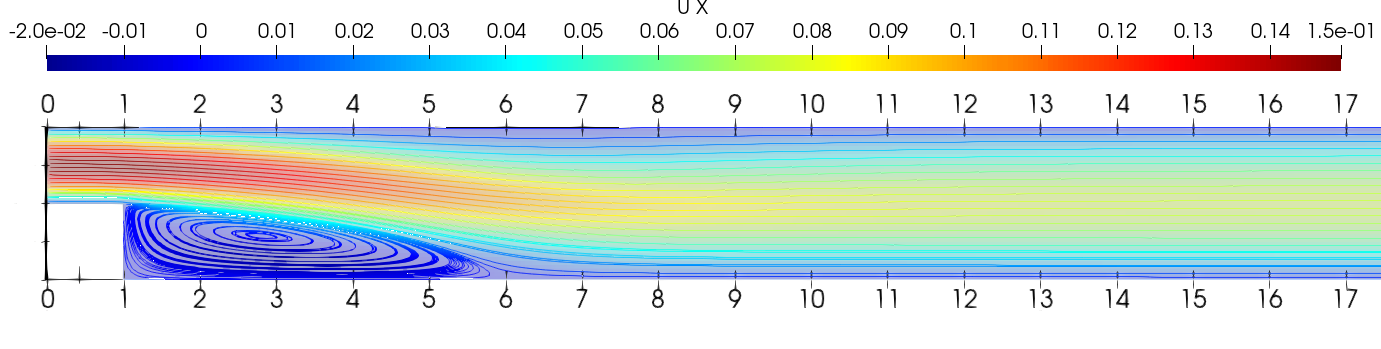
\includegraphics[scale=0.4]{pics/Re100.png}
        \caption{Re=100}
    \end{subfigure}
    \begin{subfigure}{\textwidth}
        \centering
        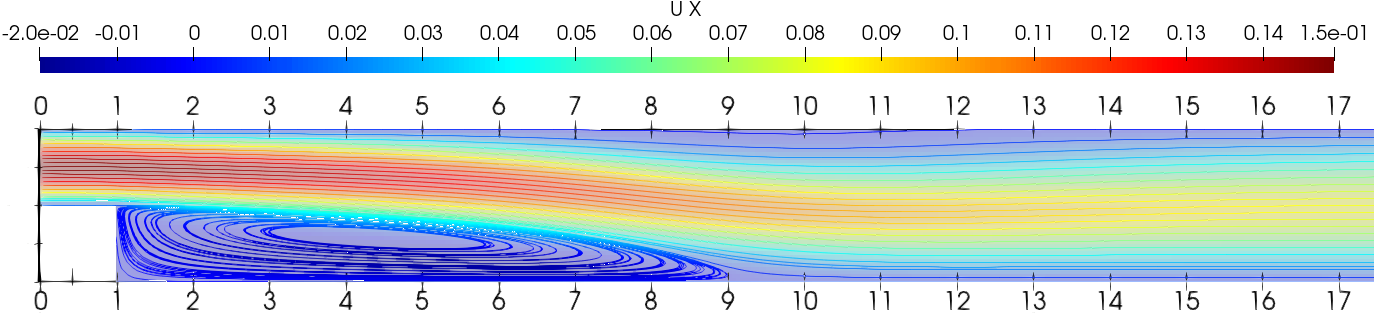
\includegraphics[scale=0.4]{pics/Re200.png}
        \caption{Re=200}
    \end{subfigure}
    \begin{subfigure}{\textwidth}
        \centering
        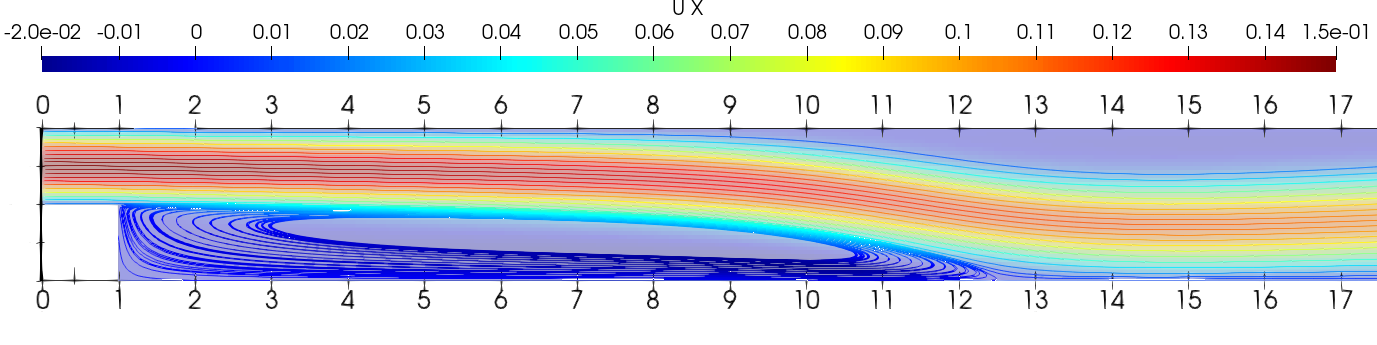
\includegraphics[scale=0.4]{pics/Re400.png}
        \caption{Re=400}
    \end{subfigure}
    \caption{Линии тока для задачи с обратным уступом}
    \label{StreamRe100}
\end{figure}


\begin{table}[!hb]
\caption {Сравнение результатов для задачи обратного уступа}
\noindent\begin{tabular}{l|ccc}
Research & $Re=100$ & $Re=200$  & $Re=400$ \\
\hline
QHDFoam & 5.0 & 8.25 & 11.9\\
Sparrow E. M. and Chuck W.\cite{Sparrow1987} & 5.0 & 7.5 & -\\
Kim J. and Moin P.\cite{Kim1985} & 5.0 & 8.3 & 12 \\
Hackman L. P. et al.\cite{Hackman1984} & 5.0 & 8.5 & -\\
\hline
Armaly B. F. et al.\cite{Armaly1983} & 5.0 & 8.5 & 14.2
\end{tabular}
\label{table:tabBackward}
\end{table}

\paragraph{Естественная конвекция}

Рассматривается задача естественной конвекции в каверне согласно \cite{ElizarBook} значение регуляризационного параметра было вычислено пропорционально обратному числу Грастгофа $Gr^{-1}$, которое было порядка $10^{-4}$ с. Сравнение максимумов горизонтальной и вертикальной скорости с данными из \cite{ElizarBook} и \cite{Vabishevich} показывают сеточную сходимость и хорошую согласованность между QHDFoam и рассматриваемыми в работах методами. Результаты сравнения видны в таблице \ref{table:tabHotCavityHor} . Линии тока изображены на рисунке \ref{fig:Nconv}. Схему расчетной области можно увидеть на рисунке \ref{fig:convectionScratch}

\begin{table}[!hb]
\caption { Сравнение максимума горизонтальной компоненты скорости для задачи естественной конвекции.}
\noindent\begin{tabular}{l|ccc}
Mesh & $U_x$ \cite{ElizarBook} & $U_x$ \cite{Vabishevich} & $U_x$ \textit{QHDFoam} \\
\hline
$20\times20$ & 15.938 & 16.144 & 16.040\\
$40\times40$ & 16.005 & 16.262 & 16.410\\
$80\times80$ & 16.070 & 16.219 & 16.225
\end{tabular}
\label{table:tabHotCavityHor}
\end{table}

 \begin{table}[!h]
\centering
\caption {Сравнение максимума вертикальной компоненты скорости для задачи естественной конвекции.}
\noindent\begin{tabular}{l|ccc}
Mesh & $U_y$ \cite{ElizarBook} & $U_y$ \cite{Vabishevich} & $U_y$ \textit{mulesQHDFoam} \\
\hline
$20\times20$ & 19.513 & 19.363 & 19.670\\
$40\times40$ & 19.663 & 19.602 & 19.910\\
$80\times80$ & 19.663 & 19.648 & 19.757
\end{tabular}
\label{table:tabHotCavityVer}
\end{table}

\begin{figure}
    \centering
    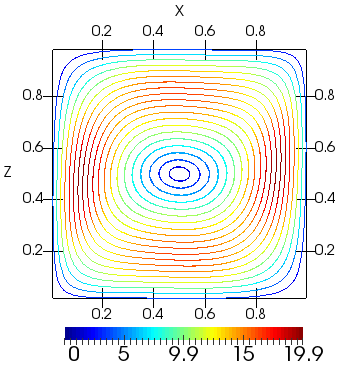
\includegraphics[scale=0.9]{pics/Umag.png}
    \caption{Линии тока для задачи естественной конвекции}
    \label{fig:Nconv}
\end{figure}

\begin{figure}
    \centering
    \begin{tikzpicture}[scale = 4]
        \draw[thick] (0,0,0) -- (1,0,0) -- (1,1,0) -- (0,1,0) -- cycle;
        
        \draw[thick, color = red] (0,0,0) -- (0,1,0);
        
        \draw[thick, color = blue] (1,0,0) -- (1,1,0);
        \draw (0.95,0.75) node[left,rotate=90] {$T=0^{\circ}$};
        
        \draw [<->,>=stealth](-0.025,0)--(-0.025,1);
        \draw (-0.075,0.9) node[left,rotate=90] {$L=1 m,$  $T=1^{\circ}$};
        
        \draw [<->,>=stealth](0,1.025)--(1,1.025);
        \draw (0.5,1.025) node[above] {$L=1 m$};
        \draw[ very thick,->, >=stealth] (0.15,0.9)  ++ (-50:.75) arc (300:-50:.25 and .25);
        
    \end{tikzpicture}
    \caption{Схематичное изображение задачи для естественной конвекции}
    \label{fig:convectionScratch}
\end{figure}

\subsection{Валидация}


Аттрактор внутренних волн -- это сложное явление, которое происходит после многократного отражения внутренних волн от стенок резервуара. PISO алгоритмы из предыдущего раздела не справляются с моделированием этого феномена, но результаты моделирования аттрактора с помощью решателя QHDFoam показывают неплохие результаты. Удалось добиться ошибки меньше 3\% см. Рис. \ref{fig:AdamsBashforthEulerNek3D}.

\begin{figure}[hbt!]
    \centering
        
    \begin{tikzpicture}[scale = 1,spy using outlines={circle, magnification=6, connect spies}]
        \begin{axis}
            [scale only axis, xlabel=Линия пробы $m \cdot 10^{-3}$, ylabel=$U_x\;\; m/s \cdot 10^{-3}$, grid=major,legend style={at={(0,1),font=\LARGE},anchor=north west}, ymin=-0.8, ymax=0.8,xmin=0,xmax=20,legend style={nodes={scale=0.5, transform shape}}, x post scale=1.6]

            \addplot[solid,color=black,thick] table [x=Points:1, y=U, col sep=comma] {CSV/NEK5000.csv};
            \addplot[solid,color=red,thick] table [x=Points:1, y=U, col sep=comma] {CSV/QHD480x320.csv};
            \addplot[solid,color=green!60!black,thick] table [x=Points:1, y=U, col sep=comma] {CSV/QHD240x160.csv};
            \addplot[solid,color=blue,thick] table [x=Points:1, y=U, col sep=comma] {CSV/QHD240x1602tau.csv};
            \legend{NEK500,QHDFoam 480x320, QHDFoam 240x160, QHDFoam 240x160 $\tau \cdot 2$}

            \coordinate (spypoint) at (axis cs:14.7,0.7);
            \coordinate (magnifyglass) at (axis cs:15.5,-0.3);
        \end{axis}
        \spy [blue, size=4cm] on (spypoint) in node[fill=white] at (magnifyglass);
    \end{tikzpicture} 
    \caption{Количественное сравнение результатов моделирования}
    \label{fig:AdamsBashforthEulerNek3D}
\end{figure}


Также количественные исследования демонстрируют сходимость решения получаемое с помощью квазигидродинамических уравнений к решению полученному с помощью метода высокого порядка (см. Рис. \ref{fig:tauAttr}) в отличии от результатов полученных с помощью PISO (см. Рис. \ref{fig:PISOattr}).

\begin{figure}
    \centering
        \begin{tikzpicture}[scale = 1.1]
          \begin{axis}
             [scale only axis, grid=major,legend style={at={(0,1),font=\LARGE},anchor=north west}, ymin=-0.8*10^-3, ymax=1.7*10^-3, xmin=0.0,legend style={nodes={scale=0.5, transform shape}}, x post scale=1.5,xlabel={$y$}, ylabel={$U_x$}];
            \addplot[solid,color=red,thick] table [x=Points:1, y=U:0, col sep=comma] {CSV/Ux300.5tau.csv};
            \addplot[solid,color=green,thick] table [x=Points:1, y=-U:0, col sep=comma] {CSV/Ux301tau.csv};
            \addplot[solid,color=blue,thick] table [x=Points:1, y=U:0, col sep=comma] {CSV/Ux302tau.csv};
            %\addplot[solid,color=violet,dashed,thick] table [x=Points:1, y=-U:0, col sep=comma] {CSV/Ux30tau001200sBackward.csv};
            \legend{$\tau = 0.005$,$\tau = 0.01$,$\tau = 0.02$,Adams-Bashforth}
          \end{axis}
          \begin{axis}
            [scale only axis, ymin=-0.8*10^-1, ymax=1.7*10^-1, xmin=0.0,  yticklabels={,,},xticklabels={,,},legend style={at={(0,0.75),font=\LARGE},anchor=north west},legend style={nodes={scale=0.5, transform shape}},x post scale=1.5];
            \addplot[solid,thick] table [x=Points:1, y=x_velocity, col sep=comma] {CSV/Ux30Nek500T200.csv};
            \legend{NEK5000}
          \end{axis}
        \end{tikzpicture} 
    \caption{Распределение скорости вдоль линии AB. Демонстрируется сходимость по $\tau$.}
    \label{fig:tauAttr}
\end{figure}


\section{Критические частоты и диапазон существования аттракторов внутренних волн}

Для фокусировки внутренних гравитационных волн используется стратифицированная жидкость с линейным профилем стратификации и трапециевидный резервуар, который может, служит линзой для внутренних гравитационных вол и фокусировать их в аттракторы внутренних гравитационных вол. При этом эффект фокусировки зависит от угла распространения внутренних волн и геометрических параметров резервуара. Аттрактор образуется далеко не при каждой комбинации этих параметров. Возможные геометрии резервуаров подробно описаны в работе Лео Мааса\cite{Maas1995}. Также там описывается процедура перехода к универсальным координатам $(d,\tau)$ это резко сокращает количество определяющих задачу параметров. Предполагается, что параметры резервуара являются фиксированными, а варьируется лишь частота колебания волнопродуктора причем этого достаточно чтобы управлять формой аттрактора. В данном разделе осуществляется поиск универсальных частот волнопродуктора, которые бы обеспечивали образование аттрактора внутренних гравитационных волн. 

Для поиска использовалась диаграмма из работы Лео Мааса\cite{Maas1997}. Найдем такие параметры системы, чтобы аттрактор вырождался в отрезки для этого положим $\tau=2$. Выбор такого значения обусловлен углом распространения внутренних волн $\theta = 45^{\circ}$. Это значит, что волна пущенная из левого верхнего угла упрется в правый нижний угол так как длинна резервуара $=2$ от $-1$ до $1$(см рис. \ref{fig:trivAttr}). Если в уравнение (\ref{eq:transformZ}) подставить вместо $z$ высоту резервуара $H$ то получим:

\begin{equation}
    \tau=\frac{2H}{L} \sqrt{\frac{N^2}{\omega^2}-1}.
\end{equation}

Теперь подставим $\tau=2$:

\begin{equation}
    1=\frac{H}{L} \sqrt{\frac{N^2}{\omega^2}-1}.
\end{equation}

Выразим отсюда $\omega$:

\begin{equation}
    \omega=\frac{NH}{\sqrt{L^2+H^2}}.
\end{equation}

\begin{figure}
    \centering
    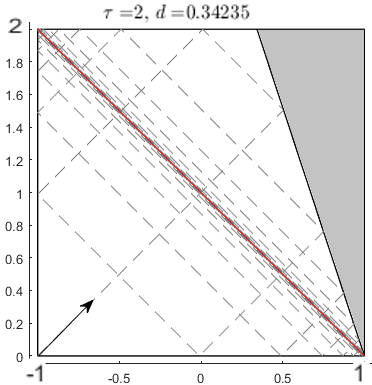
\includegraphics[scale=0.8]{Figs/CritAttrFreq.png}
    \caption{Вырожденный аттрактор внутренних волн.}
    \label{fig:trivAttr}
\end{figure}

Теперь найдем второй случай, при котором аттрактор зажимается между двумя противоположными углами. Это означает что луч пущенный из левого нижнего угла должен попасть в точку $d$. То есть $\tau = 1+d$:

\begin{equation}
    1+d=\frac{2H}{L} \sqrt{\frac{N^2}{\omega^2}-1}.
\end{equation}

Выразим отсюда частоту $\omega$:

\begin{equation}
    \omega = \frac{NH}{\sqrt{\left( 1-H\cdot tg(\alpha) \right)^2+H^2}}.
\end{equation}

После процедуры рейтрейсинга(см рис. \ref{fig:attrTriv})
    
\begin{figure}
    \centering
    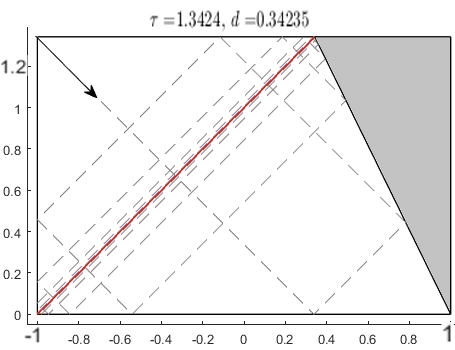
\includegraphics[scale=0.6]{Figs/AttrCritFreq.png}
    \caption{Вырожденный аттрактор внутренних волн.}
    \label{fig:attrTriv}
\end{figure}


Также с помощью метода спектральных элементов случаи вырожденных аттракторов были смоделированы(см. рис. \ref{fig:critNekfr}).

\begin{figure}
    \centering
    
    \begin{subfigure}[с]{1\textwidth}
        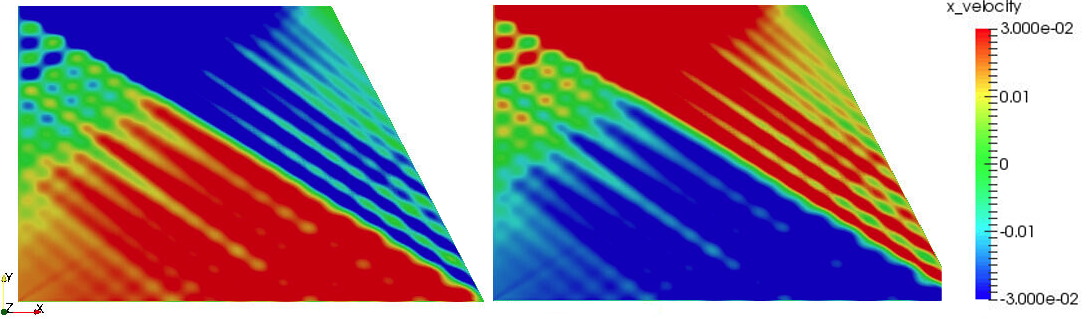
\includegraphics[scale=0.45]{Figs/AttrNEKcrit1.png}
        \caption{Расчет при помощи метода спектральных элементов с первой критической частотой}
    \end{subfigure}
    
    \begin{subfigure}[r]{1\textwidth}
        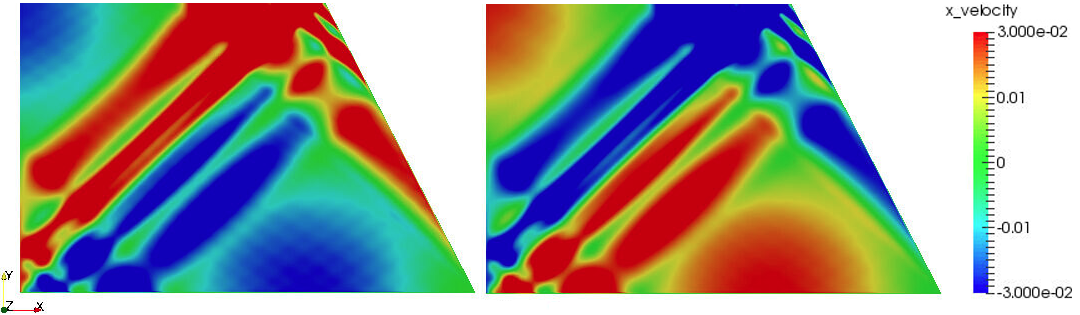
\includegraphics[scale=0.45]{Figs/AttrNekCrit2.png}
        \caption{Расчет при помощи метода спектральных элементов со второй критической частотой}
    \end{subfigure}
    \caption{Результаты расчетов при колебании волнопродуктора с критическими частотами}
    \label{fig:critNekfr}
\end{figure}

Критические значения замыкают собой диапазон частот, колебания волнопродуктора с которыми будет приводить к образованию аттрактора:

\begin{equation}
    \omega_{c_{1}}=\frac{NH}{\sqrt{L^2+H^2}}, \;\;\;\;\;\;\;\;\; \omega_{c_{2}} = \frac{NH}{\sqrt{\left( 1-H\cdot tg(\alpha) \right)^2+H^2}},
\end{equation}


\begin{equation}
    \omega_{c_{1}} \leq \omega_A \leq \omega_{c_{2}}.
\end{equation}

Этот раздел дает ответ на вопрос о том какие частоты приводят к образованию аттрактора внутренних гравитационных волн в резервуаре. Эти частоты зависят только от геометрических параметров резервуара и частоты плавучести.

\section{Волновые движения в замкнутом резервуаре при воздействии с двумя частотами}

Известно, что в океане существует великое множество волн. Вопрос будут ли волны различных частот мешать образовываться аттрактору до сих пор остается открытым. В данной работе изучается вопрос совместного воздействия на стратифицированную жидкость волнопродуктора с двумя различными частотами и одинаковой амплитудой. 

Постановка задачи несколько меняется. Для моделирования используется конфигурация представленная на рисунке \ref{fig:domainup}. Условие на волнопродукторе будет теперь записываться следующим образом:

\begin{equation}
    U_z = A_1\cdot cos\left(\frac{\pi \cdot z}{L_1}\right)\cdot \omega_1 \cdot  sin(\omega_1 t) + A_2\cdot cos\left(\frac{\pi \cdot z}{L_1}\right)\cdot \omega_2 \cdot  sin(\omega_2 t)
\end{equation}

Посчитаны различные режимы:

\begin{itemize}
    \item Режим разнесенными частотами, $\omega_1/N=0.58$ $\omega_2/N=0.66$ и малой амплитудой $a=0.02$ см. 
    \item Режим с совпадающими частотами, $\omega_1=\omega_2=0.628$ и амплитудой $a=0.05$ см.
    \item Режим с приближенными частотами, $\omega_1/N=0.66$ $\omega_2/N=0.68$ и амплитудой $a=0.05$ см.
    \item Режим с близкими частотами $\omega_1/N=0.628$ $\omega_2/N=0.641$ и  амплитудой $a=0.05$ см.
\end{itemize}

Первый режим демонстрирует общую картину течения при взаимодействии с двумя частотами. На рисунке \ref{fig:biharmVyamp02} показано, что в одном резервуаре допустимо существования сразу двух аттракторов внутренних волн. Это видно по характерному распределению поля скоростей и давлений в резервуаре. В середине первого(том что соединяет нижнюю и наклонную стенку) луче аттрактора помещена точка пробы. Видно, что существует задержка между частотой колебания волнопродуктора и частотой колебаний в середине первого луча аттрактора. Помимо этого, построен спектр частот колебаний скорости, частоты на этом графике осреднены по большей из частот. Сама точка пробы также размещена на первом луче аттрактора, который возникает под воздействием большей из частот. Это объясняет то почему второй пик меньше. На протяжении всей частотно-временной диаграммы наблюдается доминация этих двух частот.

\begin{figure}
  \centering
    \begin{subfigure}[с]{0.45\textwidth}
        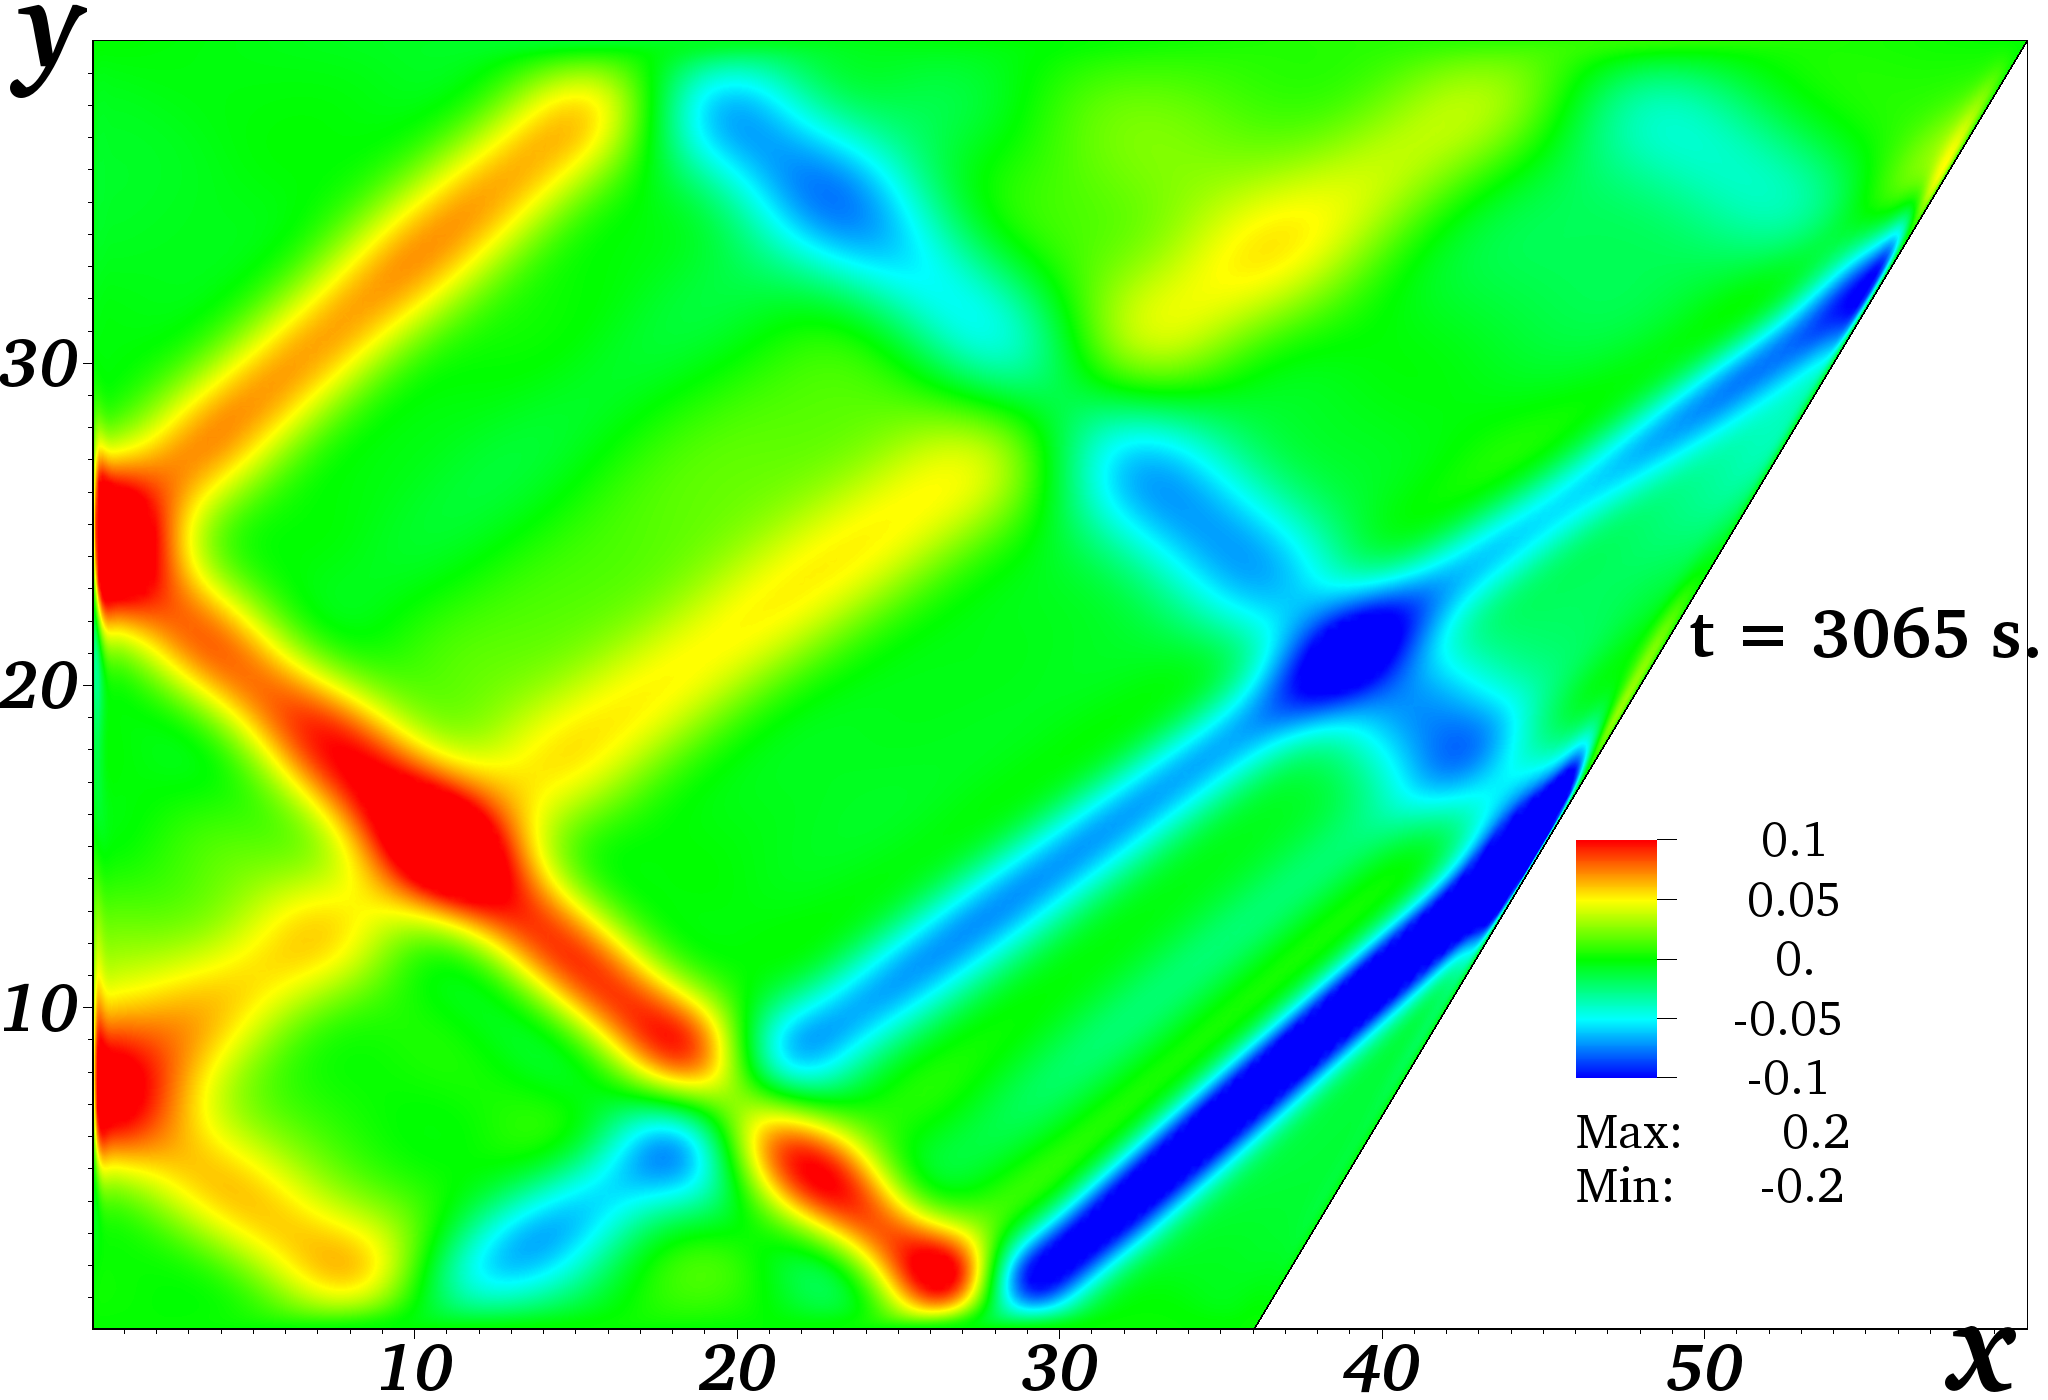
\includegraphics[width=1\textwidth]{pics/H40L60N1ap02dp20w1p58w2p66Biharm/2D36x36DiagramH40L60N1ap02dp20w1p58w2p66BiharmVyn06129.png}
        \caption{Вертикальная компонента скорости}
    \end{subfigure}
    \begin{subfigure}[с]{0.45\textwidth}
        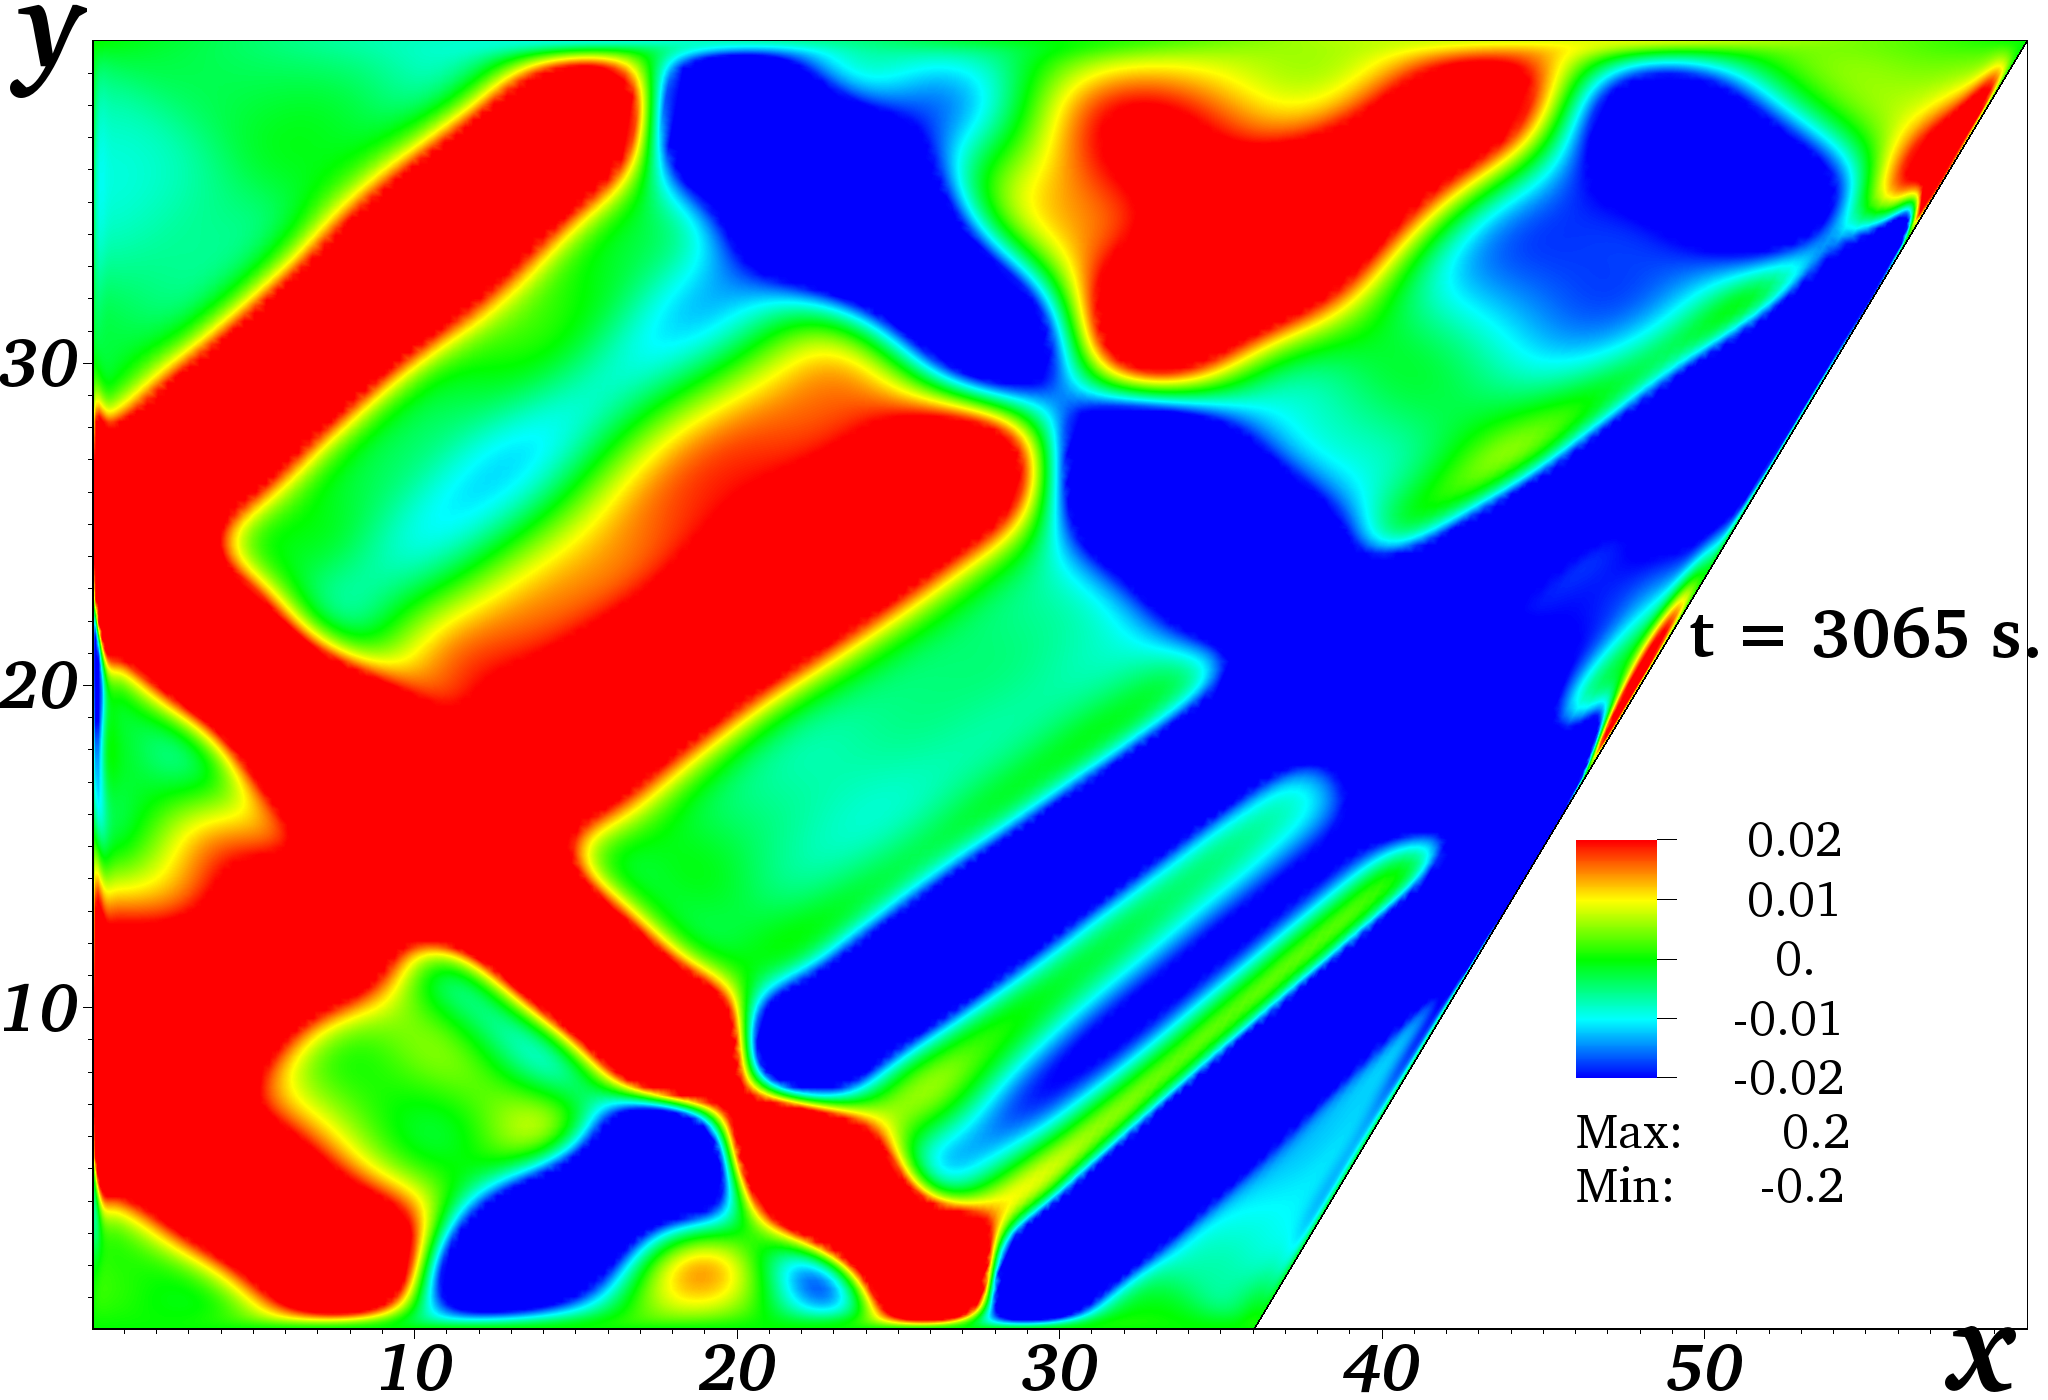
\includegraphics[width=1\textwidth]{pics/H40L60N1ap02dp20w1p58w2p66Biharm/2D36x36DiagramH40L60N1ap02dp20w1p58w2p66BiharmVy6129.png}
        \caption{Поле давления}
    \end{subfigure}
    \par
    \begin{subfigure}[с]{0.45\textwidth}
        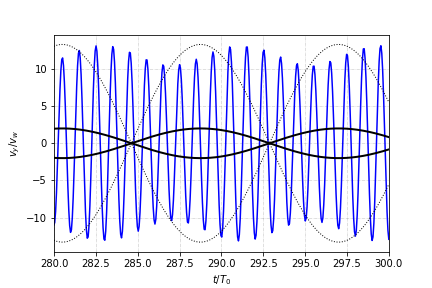
\includegraphics[width=1\textwidth]{pics/H40L60N1ap02dp20w1p58w2p66Biharm/vyX36p49Y7p94frm280to300.png}
        \caption{Вертикальная компонента скорости в середине первого луча аттрактора}
    \end{subfigure}
    \begin{subfigure}[с]{0.45\textwidth}
        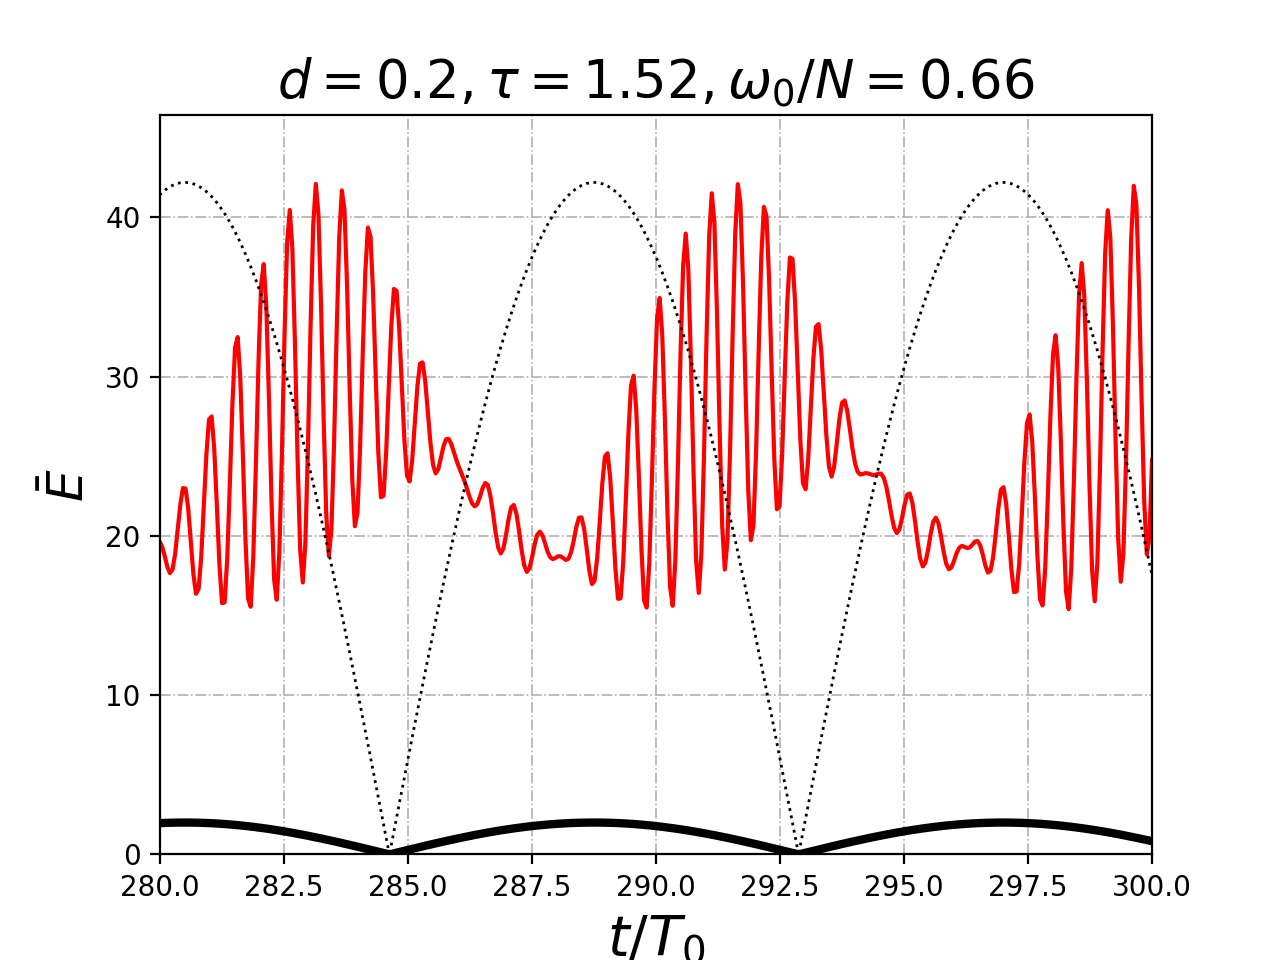
\includegraphics[width=1\textwidth]{pics/H40L60N1ap02dp20w1p58w2p66Biharm/2D36x36DiagramH40L60N1ap02dp20w1p58w2p66BiharmtotKEnonDim.png}
        \caption{Средняя кинетическая энергия в резервуаре}
    \end{subfigure}
    \par
    \begin{subfigure}[с]{0.45\textwidth}
        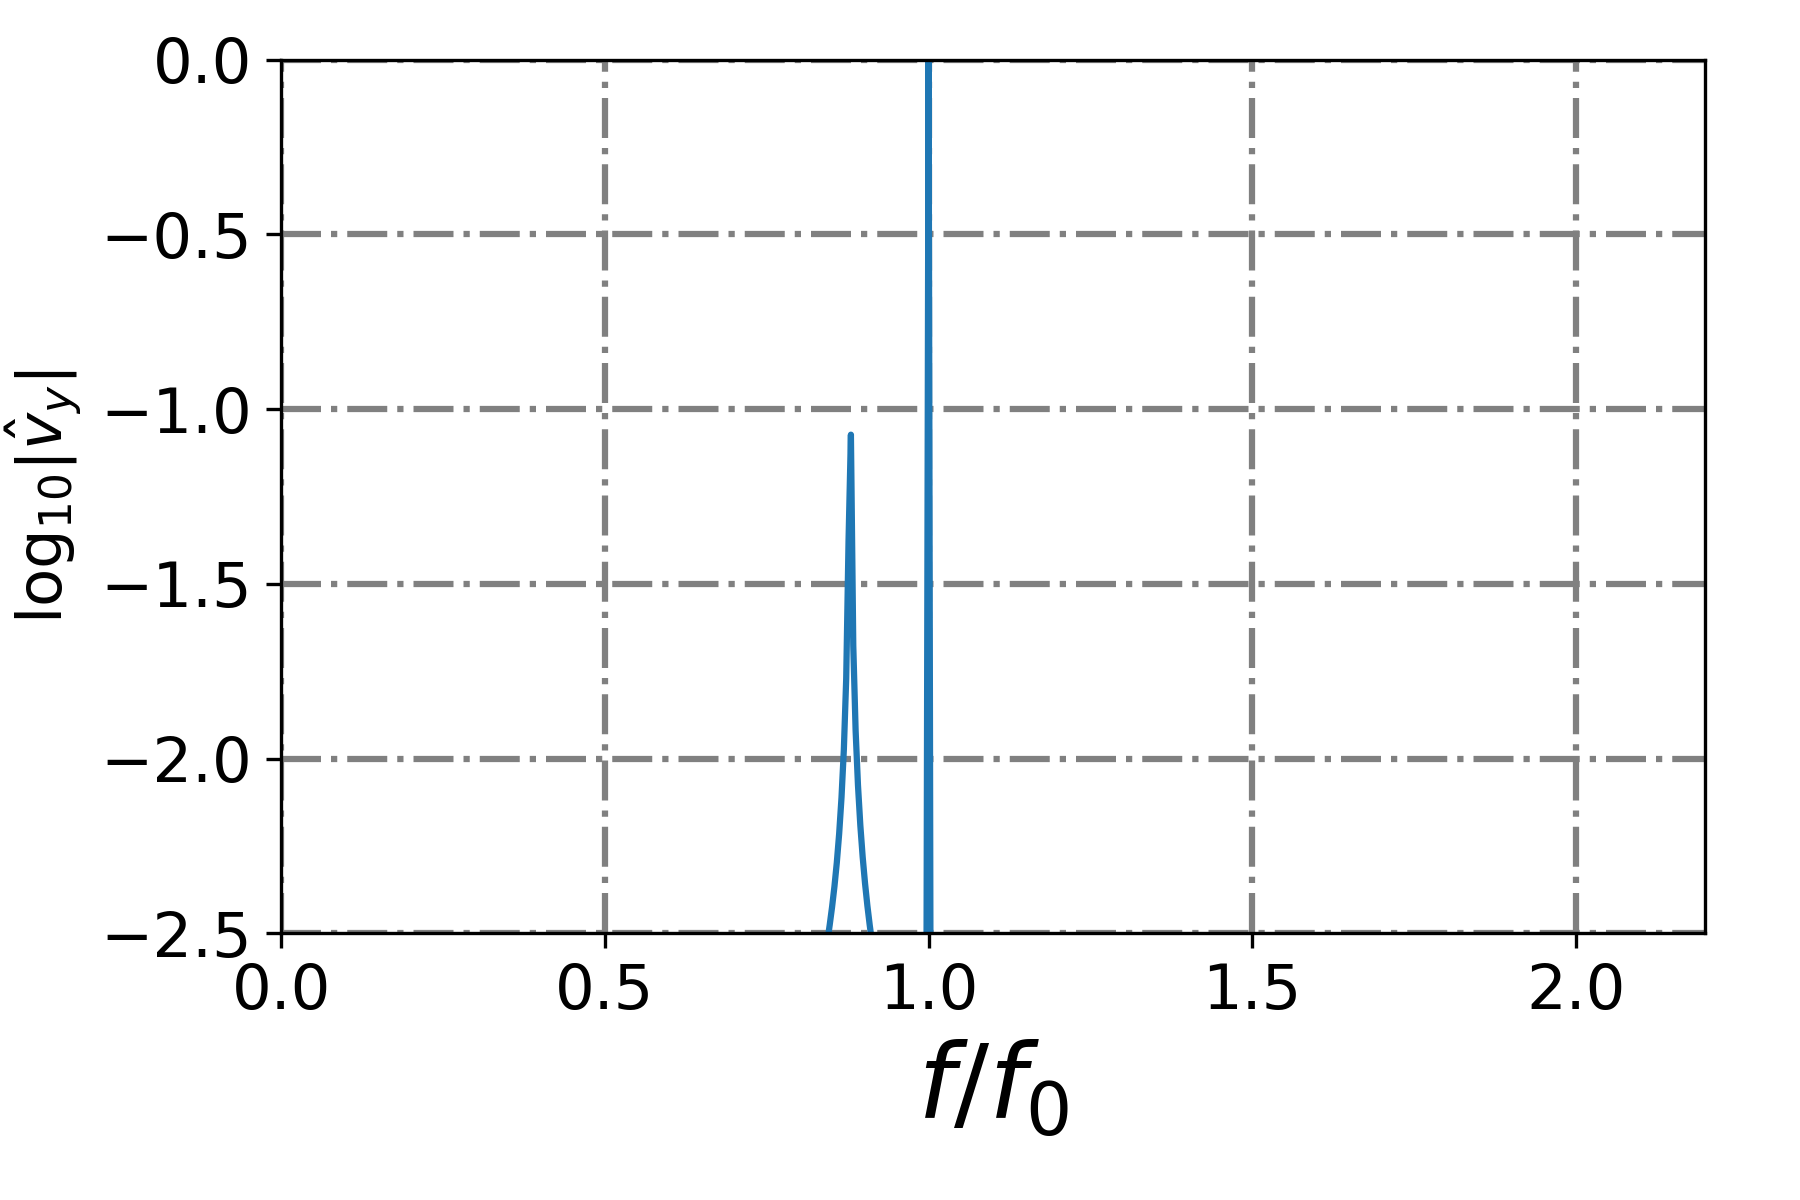
\includegraphics[width=1\textwidth]{pics/H40L60N1ap02dp20w1p58w2p66Biharm/spectrumX36p4Y8p0.png}
        \caption{Спектр}
    \end{subfigure}
    \begin{subfigure}[с]{0.45\textwidth}
        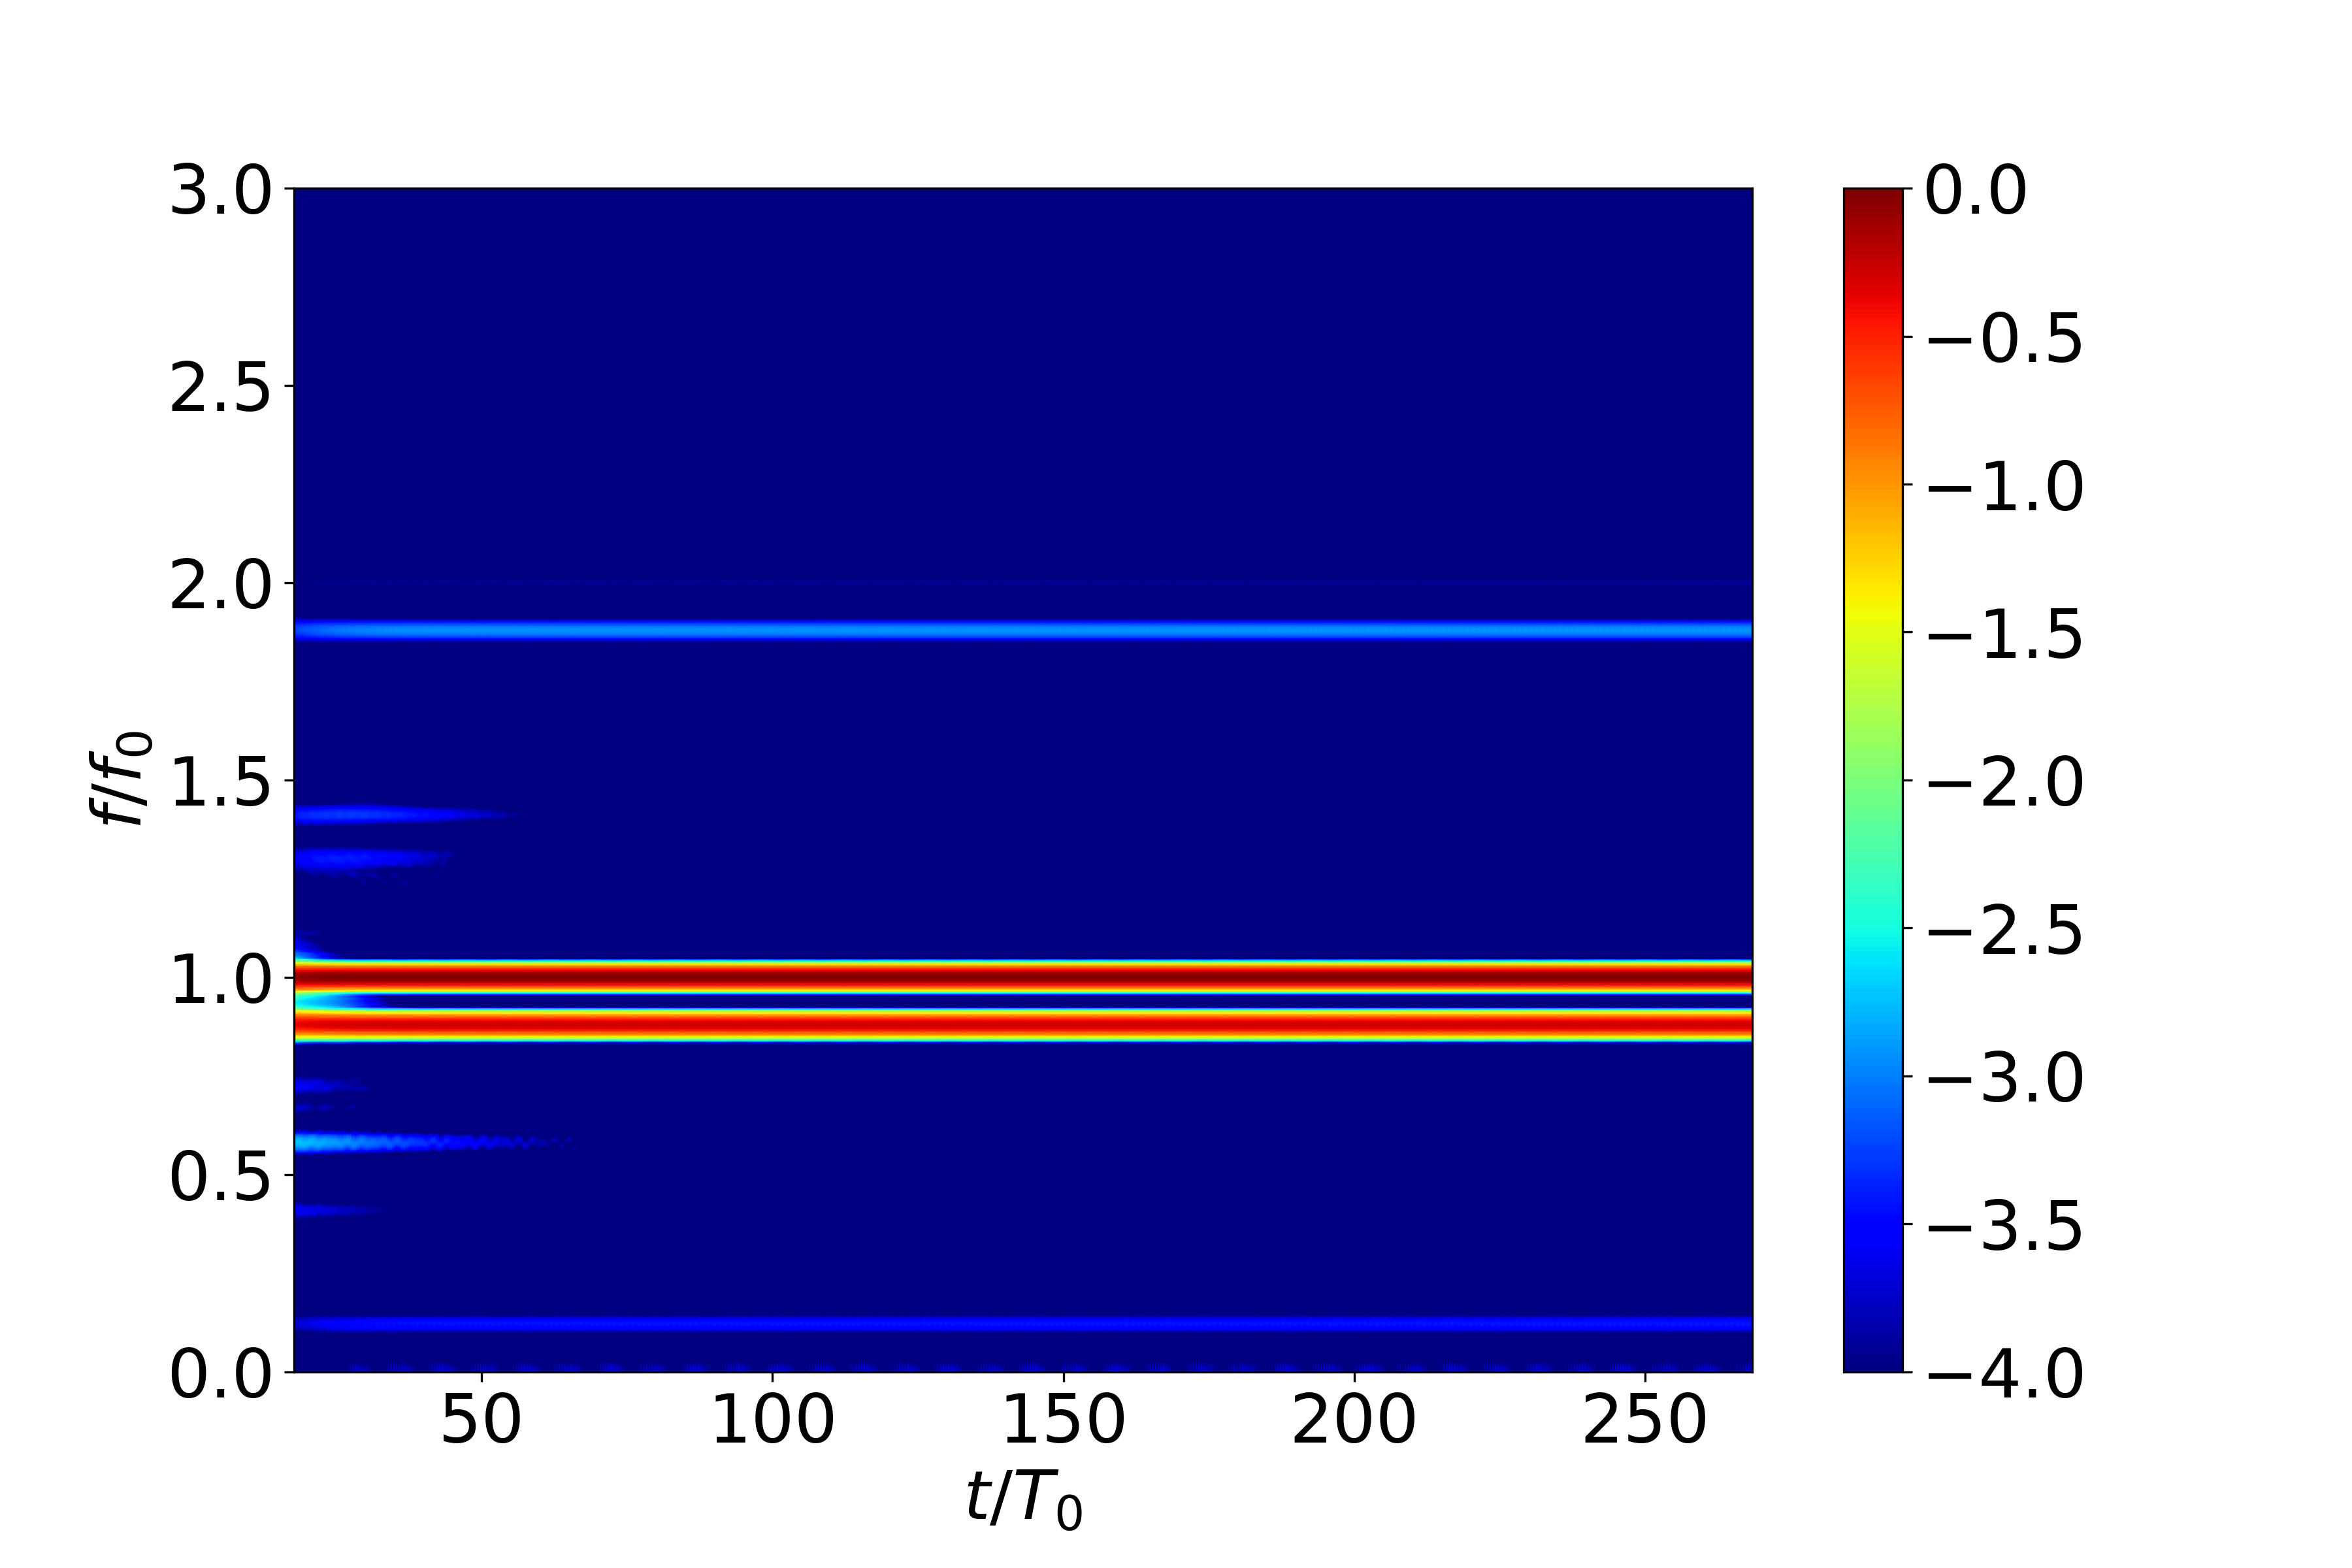
\includegraphics[width=1\textwidth]{pics/H40L60N1ap02dp20w1p58w2p66Biharm/TFspectrumX36p4Y8p0N768.png}
        \caption{Частотно-временная диаграмма}
    \end{subfigure}
    \caption{Результаты количественного исследования характеристик течения стратифицированной жидкости в трапециевидном резервуаре при внешнем воздействии с двумя разнесенными частотами $\omega_1/N=0.58$,  $\omega_2/N=0.66$. Черной линией  на графиках вертикальной скорости и кинетической энергии показана огибающая амплитуды колебаний волнпородуктора.}
    \label{fig:biharmVyamp02}
\end{figure}

Совпадение частот означает, что амплитуда колебаний удваивается значение $a=0.05$ cm. При $a=0.1$ на рисунке \ref{fig:Vyamp1} наблюдается неустойчивость этот режим характеризуется россыпью частот на спектре и частотно-временной диаграмме.

\begin{figure}
	\centering
	\begin{subfigure}[с]{0.45\textwidth}
	    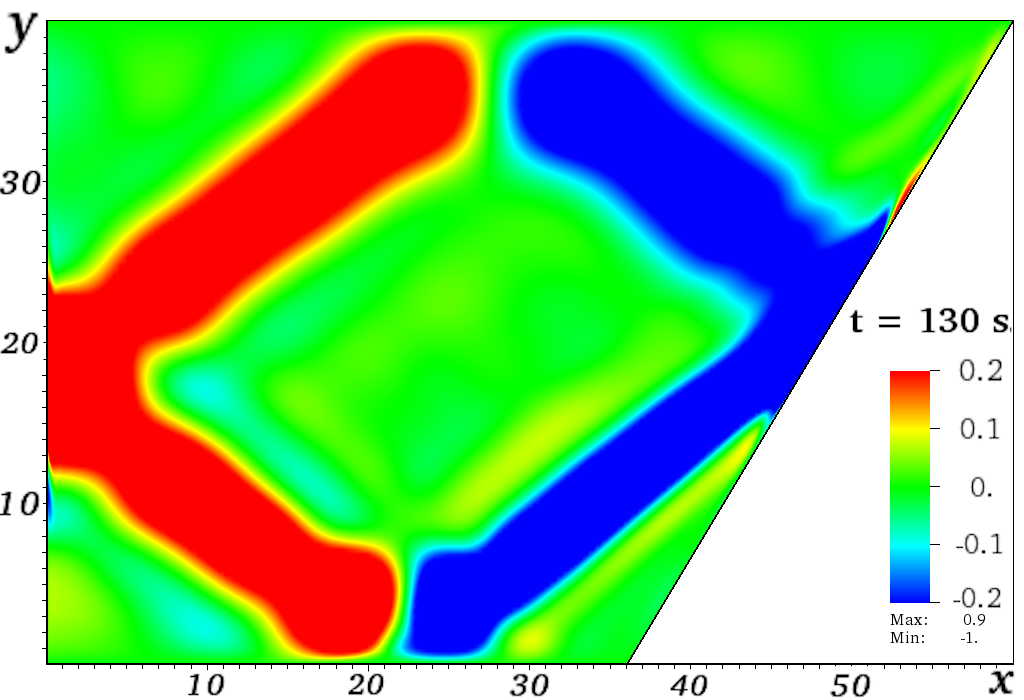
\includegraphics[width=1\textwidth]{pics/H40L60N1ap10dp20w0p63/2DH40L60N1ap10dp20w0p63Vyn00012.png}
	    \caption{Поле вертикальной скорости при образовании аттрактора}
	\end{subfigure}
	\begin{subfigure}[с]{0.45\textwidth}
	    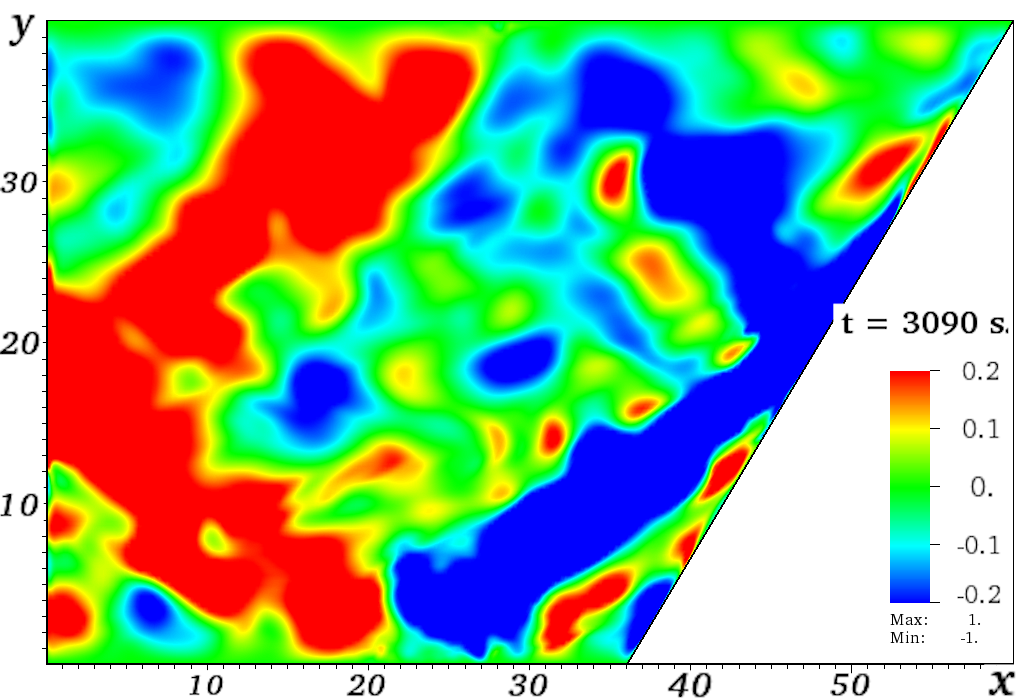
\includegraphics[width=1\textwidth]{pics/H40L60N1ap10dp20w0p63/2DH40L60N1ap10dp20w0p63Vyn00308.png}
	    \caption{Поле вертикальной скорости при образовании неустойчивостей}
	\end{subfigure}
	\par
	\begin{subfigure}[с]{0.45\textwidth}
	    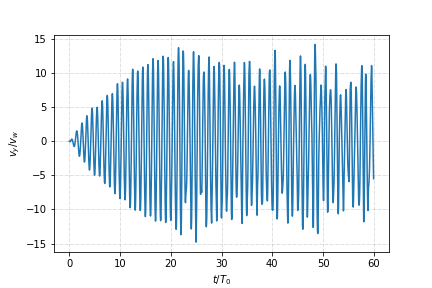
\includegraphics[width=1\textwidth]{pics/H40L60N1ap10dp20w0p63/vyX35p6Y11p3t1200.png}
	    \caption{зависимость скорости в середине первого луча аттрактора от времени}
	\end{subfigure}
	\begin{subfigure}[с]{0.45\textwidth}
	    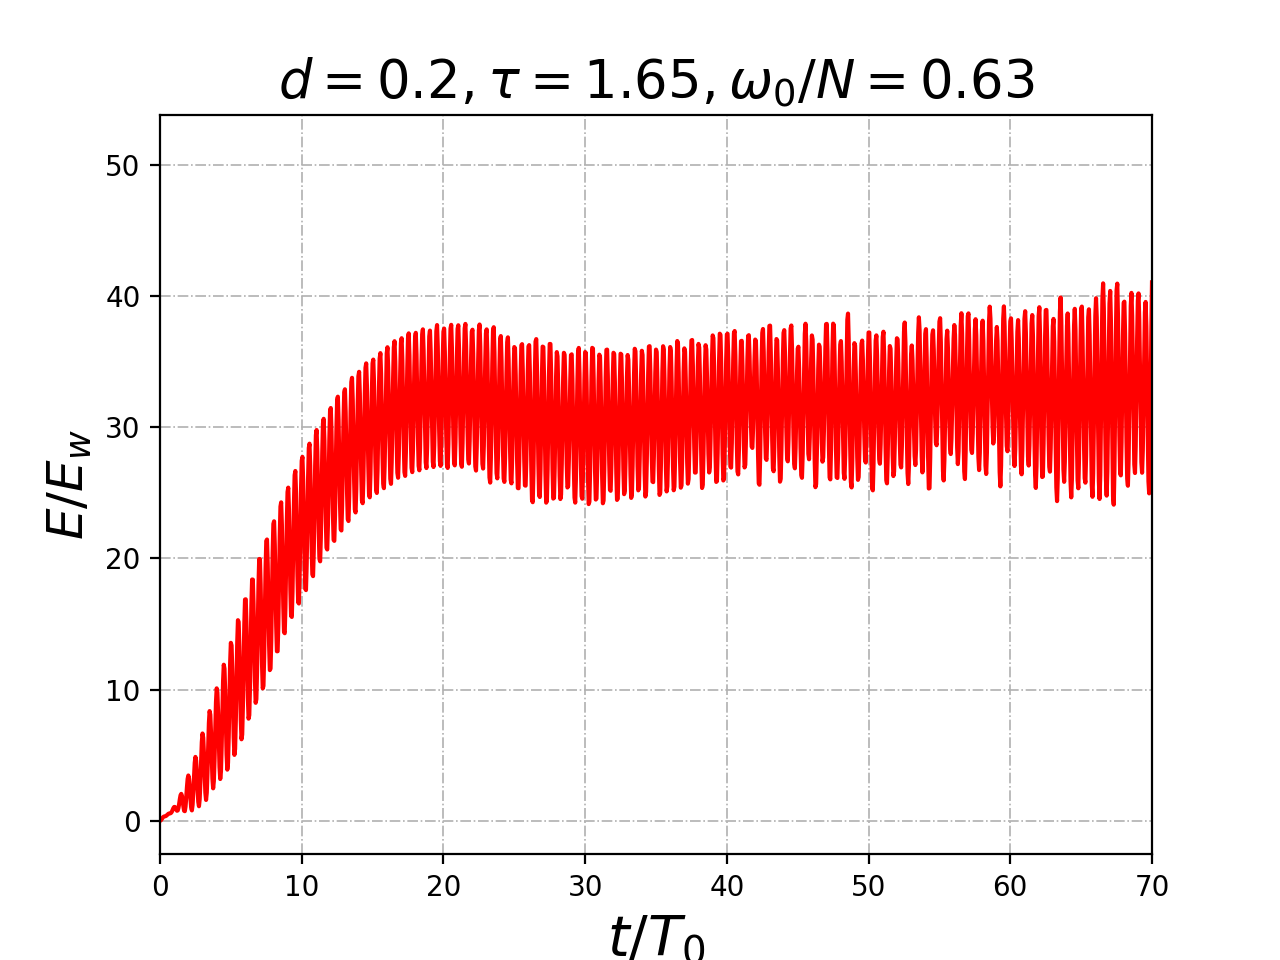
\includegraphics[width=1\textwidth]{pics/H40L60N1ap10dp20w0p63/2D36x36DiagramH40L60N1ap10dp20w0p63totKEnonDim.png}
	    \caption{Зависимость кинетической энергии от времени}
	\end{subfigure}
	\par
	\begin{subfigure}[с]{0.45\textwidth}
	    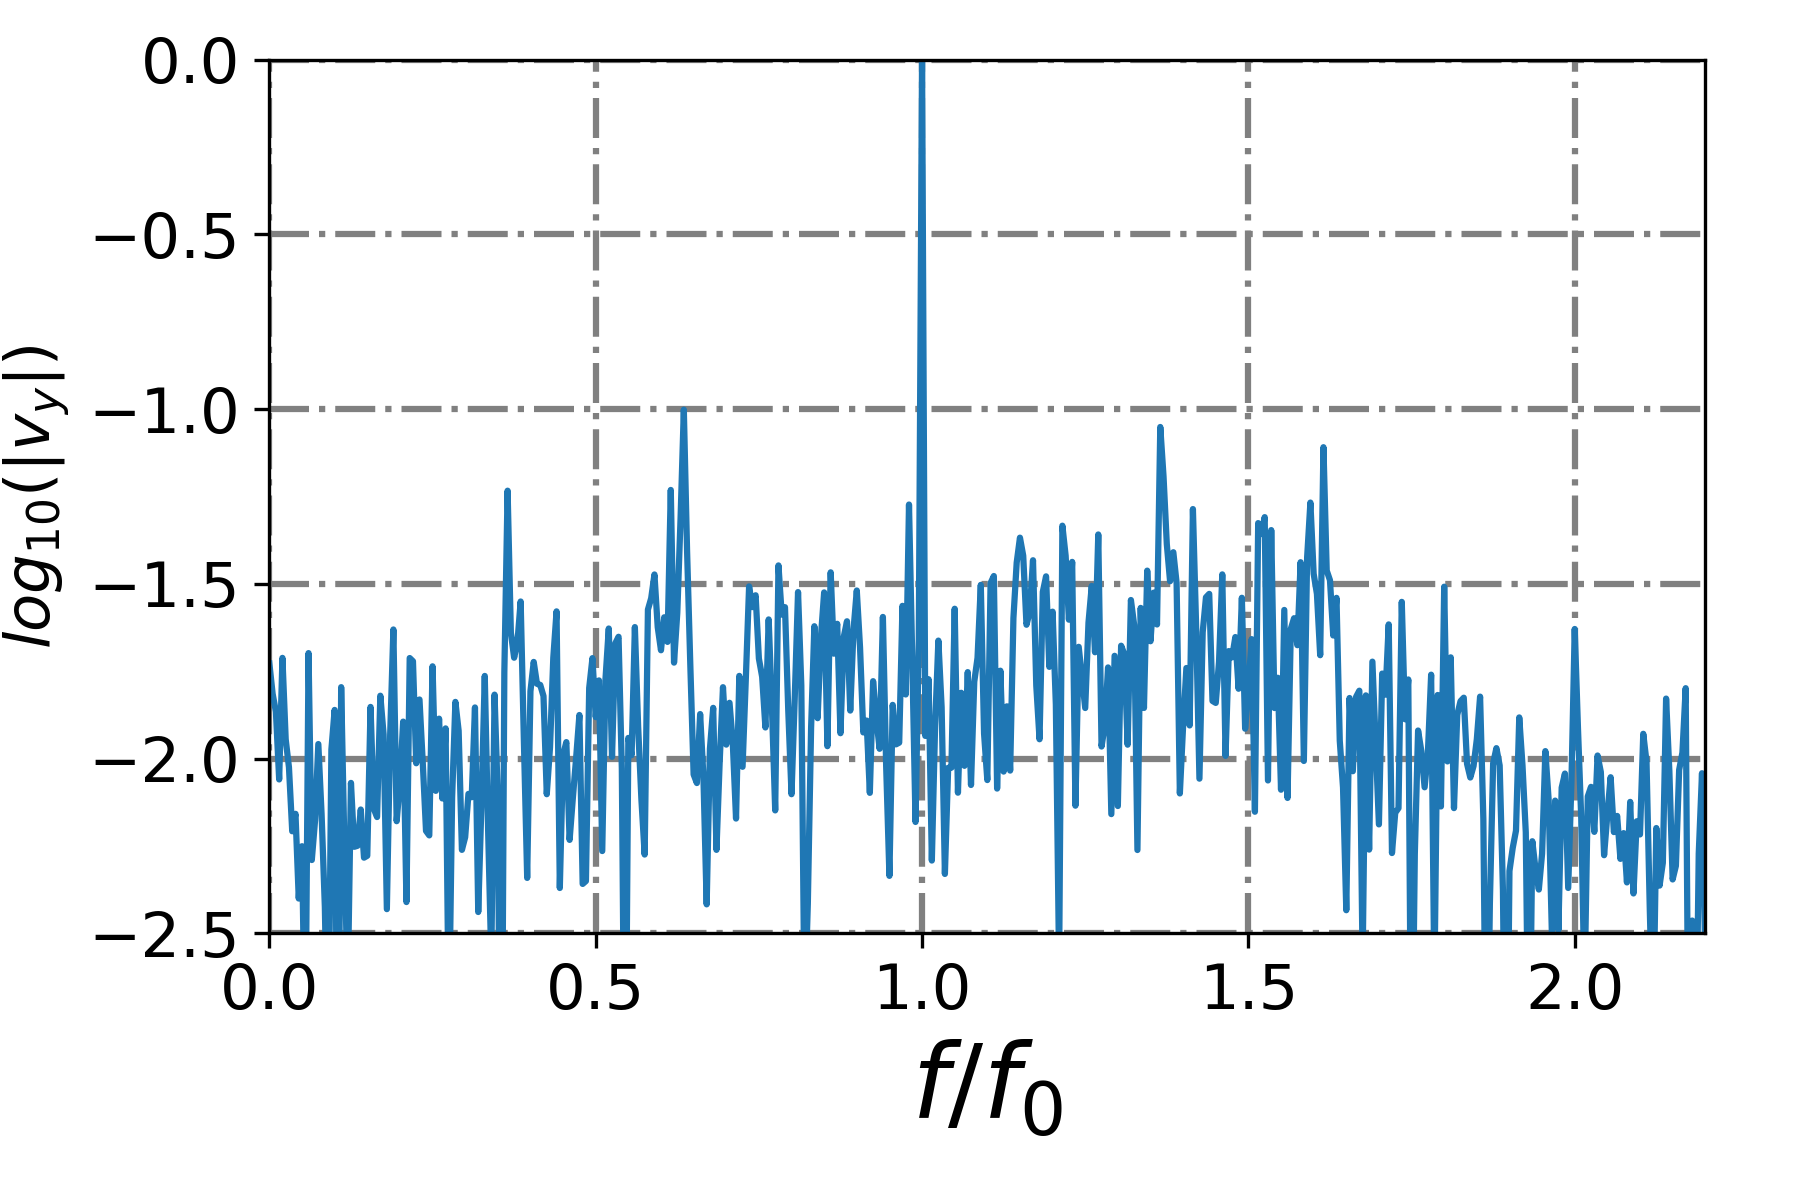
\includegraphics[width=1\textwidth]{pics/H40L60N1ap10dp20w0p63/spectrumX35p6Y11p2n4000.png}
	    \caption{Частотный спектр скорости}
	\end{subfigure}
	\begin{subfigure}[с]{0.45\textwidth}
	    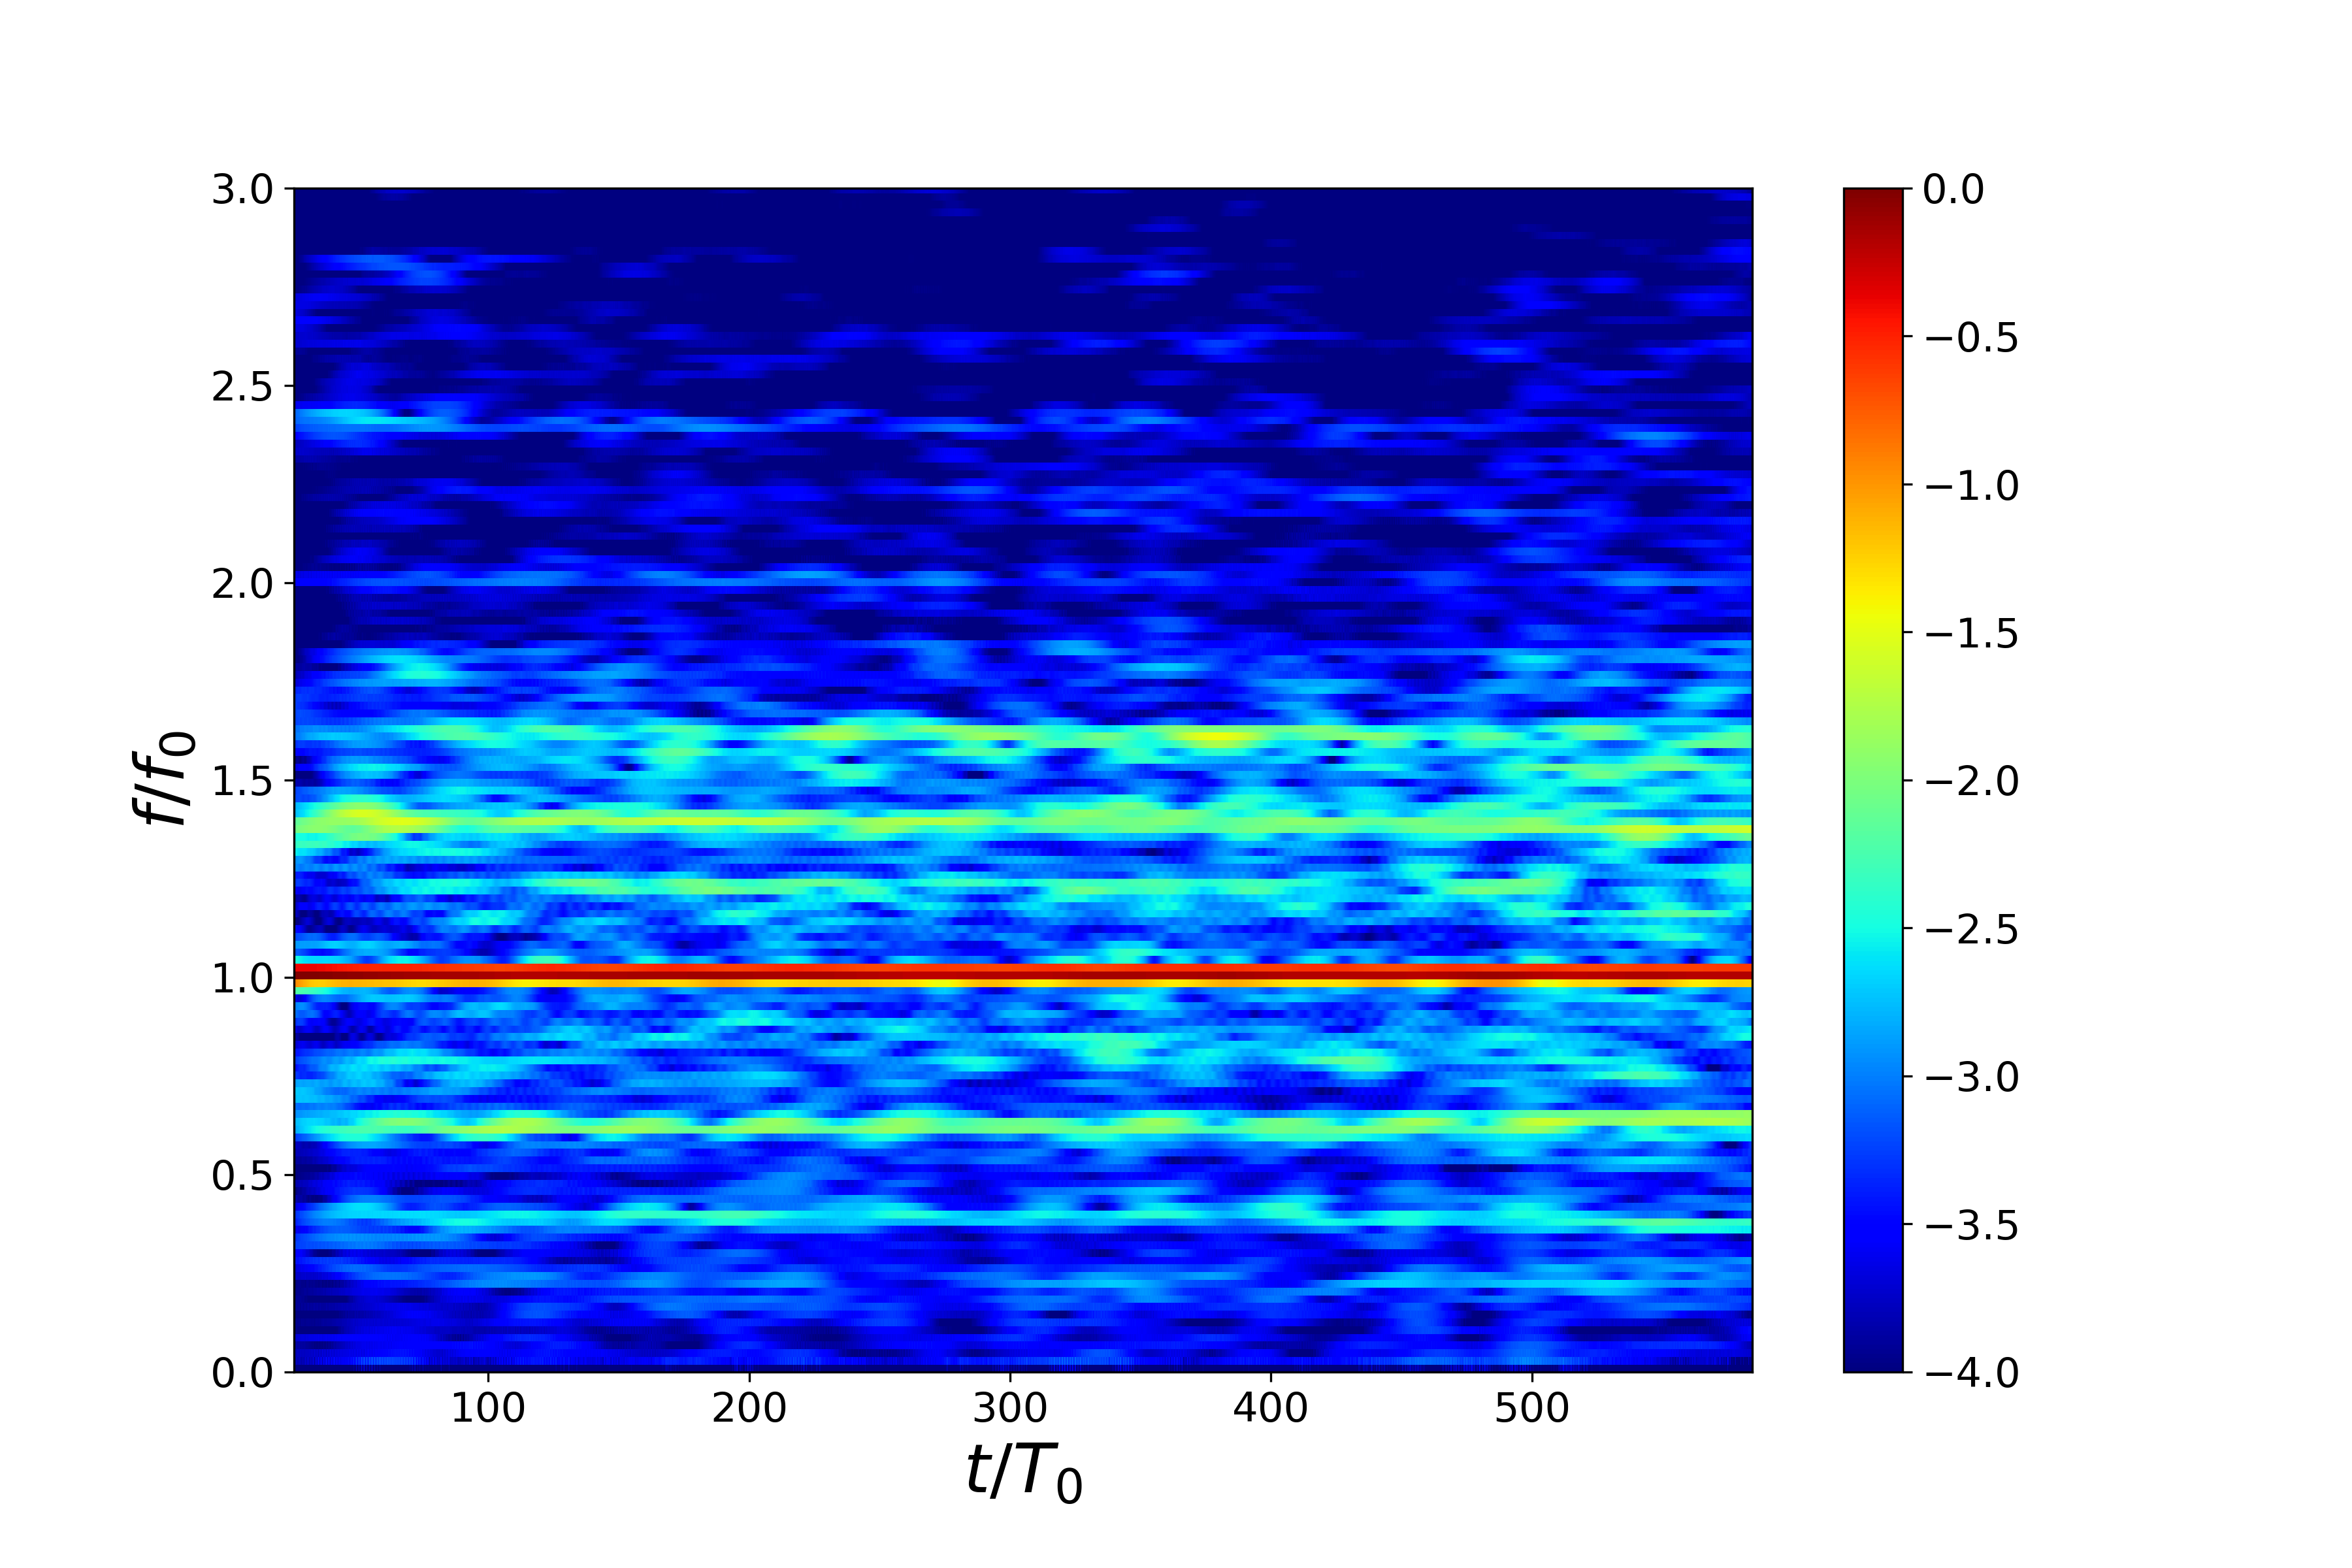
\includegraphics[width=1\textwidth]{pics/H40L60N1ap10dp20w0p63/TFspectrumX35p6Y11p2N1024.png}
	    \caption{Частотно-временная диаграмма}
	\end{subfigure}
	\label{fig:Vyamp1-1}
	\caption{Количественное исследования аттрактора с совпадающими частотами и образование неустойчивости}
	\label{fig:Vyamp1}
\end{figure}

Последующие режимы это попытка постепенно приблизить две частоты друг к другу и зафиксировать момент возникновения неустойчивости в зависимости от близости частот друг к другу. На рисунке \ref{fig:biharmVyap005-1} представлена картина течения при относительной разности частот в 0.05. При этом режиме наблюдаются дочерние волны как на изображении с вертикальной компонентой скорости, спектре так и на частотно временной диаграмме. При этом на последней наблюдаются  амплитудные <<всплески>>. Это объясняется совпадением фаз двух волновых процессов.

\begin{figure}
  \centering
  \begin{subfigure}[с]{0.45\textwidth}
    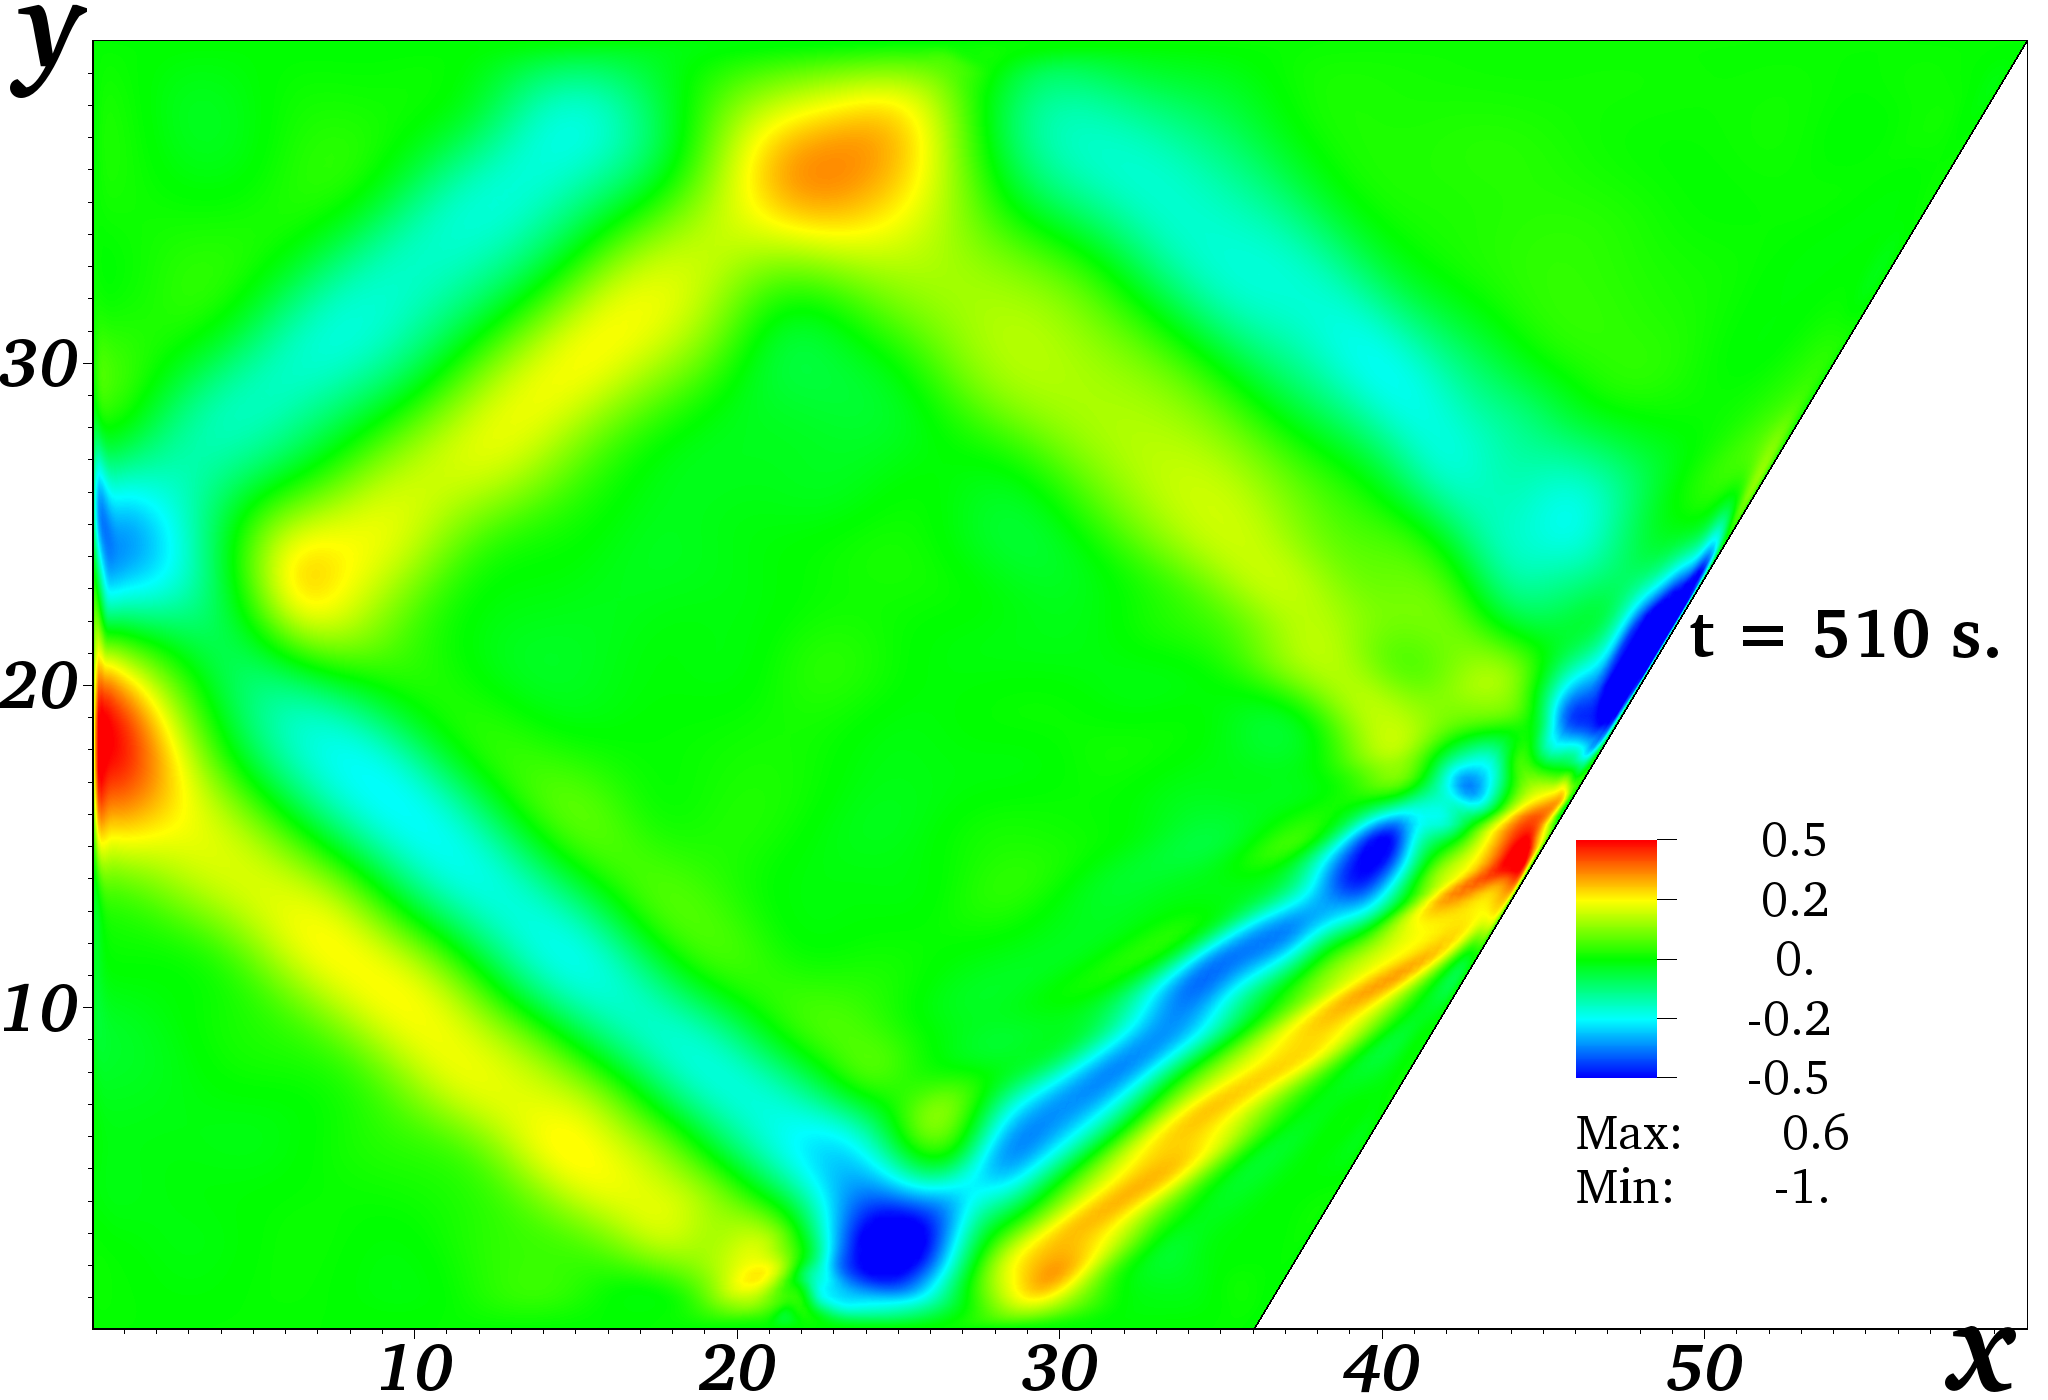
\includegraphics[width=1\textwidth]{pics/H40L60N1ap05dp20w1p63Deltawp05Biharm/2D36x36DiagramH40L60N1ap05dp20w0p63Deltawp3315BiharmVyn01019.png}
    \caption{Вертикальная компонента скорости при формировании аттрактора}
  \end{subfigure}
  \begin{subfigure}[с]{0.45\textwidth}
    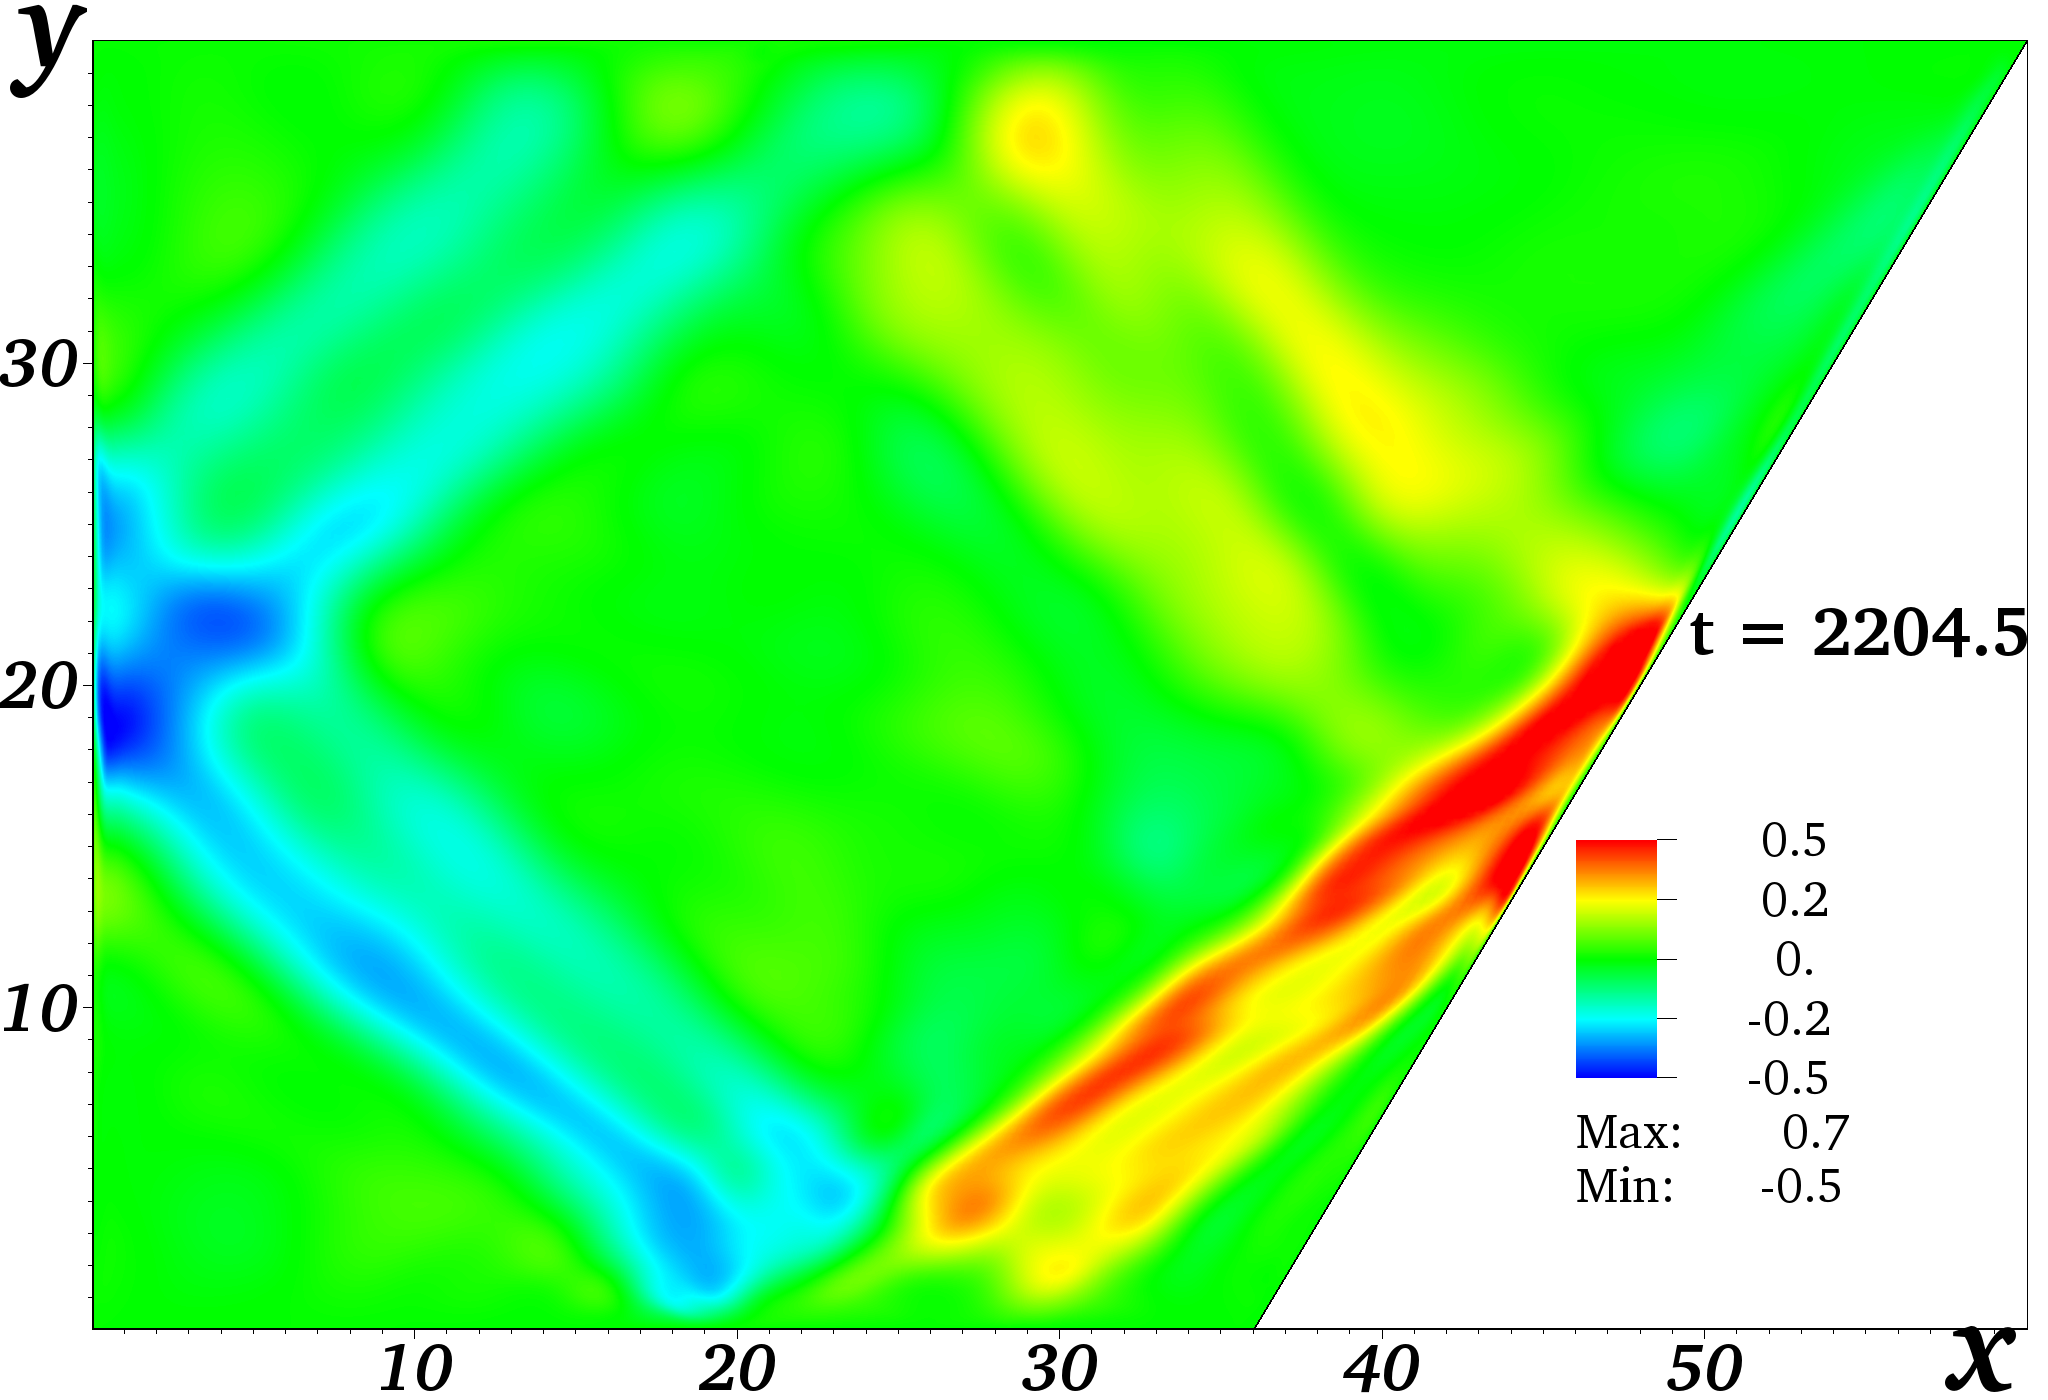
\includegraphics[width=1\textwidth]{pics/H40L60N1ap05dp20w1p63Deltawp05Biharm/2D36x36DiagramH40L60N1ap05dp20w0p63Deltawp3315BiharmVyn04408.png}
    \caption{Вертикальная компонента скорости при установлении аттрактора}
  \end{subfigure}
  \par
  \begin{subfigure}[с]{0.45\textwidth}
    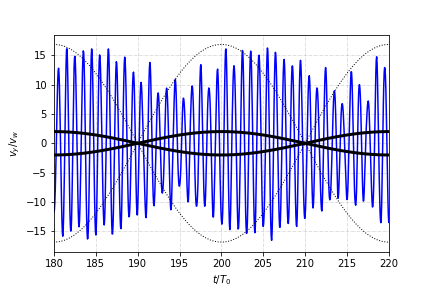
\includegraphics[width=1\textwidth]{pics/H40L60N1ap05dp20w1p63Deltawp05Biharm/vyX35p57Y11p27t4412.png}
    \caption{Вертикальная скорость}
  \end{subfigure}
  \begin{subfigure}[с]{0.45\textwidth}
    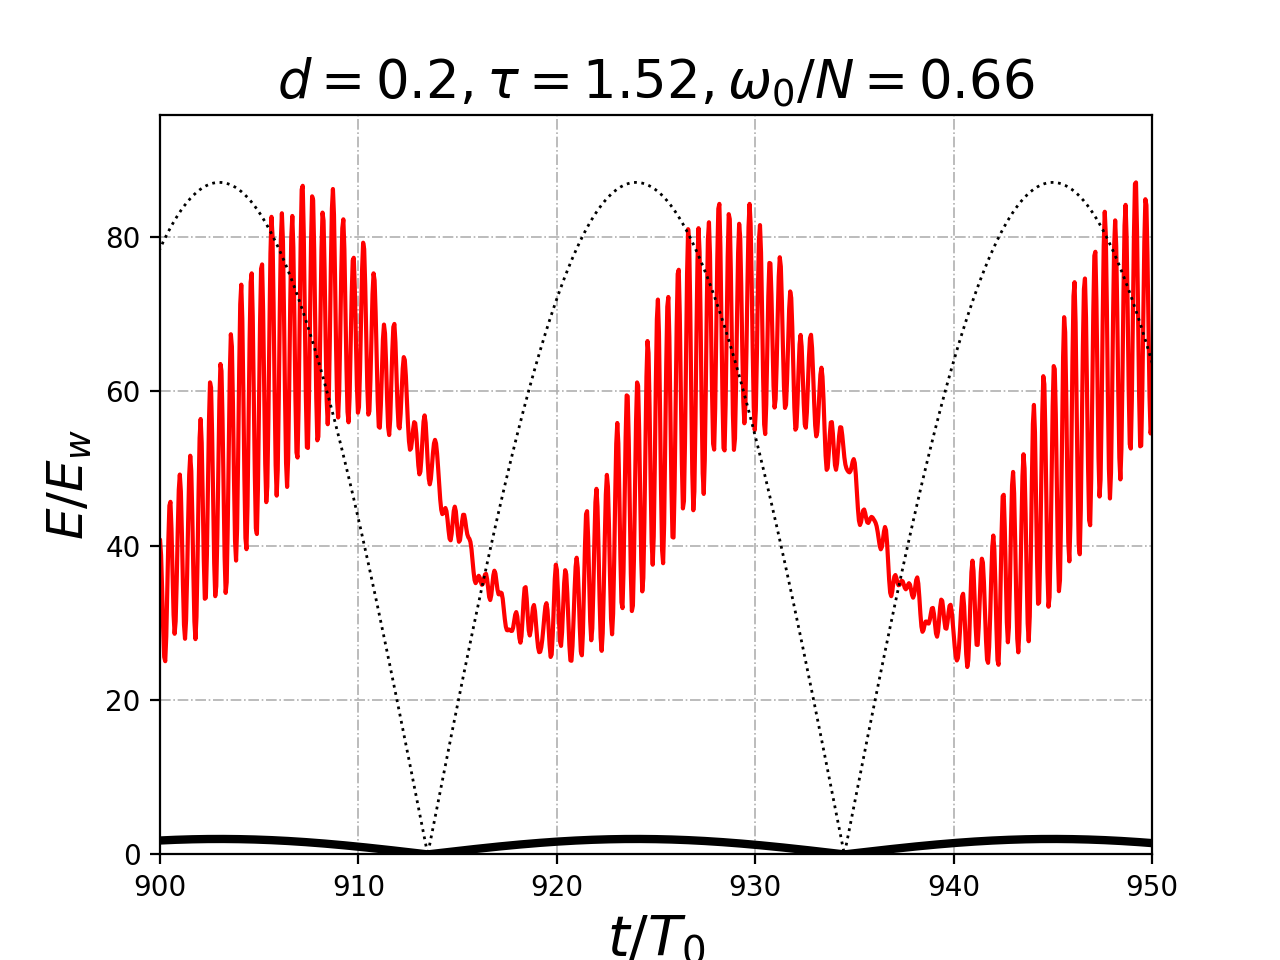
\includegraphics[width=1\textwidth]{pics/H40L60N1ap05dp20w1p63Deltawp05Biharm/2D36x36DiagramH40L60N1ap05dp20w1p63Deltawp05BiharmtotKEnonDim.png}
    \caption{Кинетическая энергия}
  \end{subfigure}
  \par
  \begin{subfigure}[с]{0.45\textwidth}
    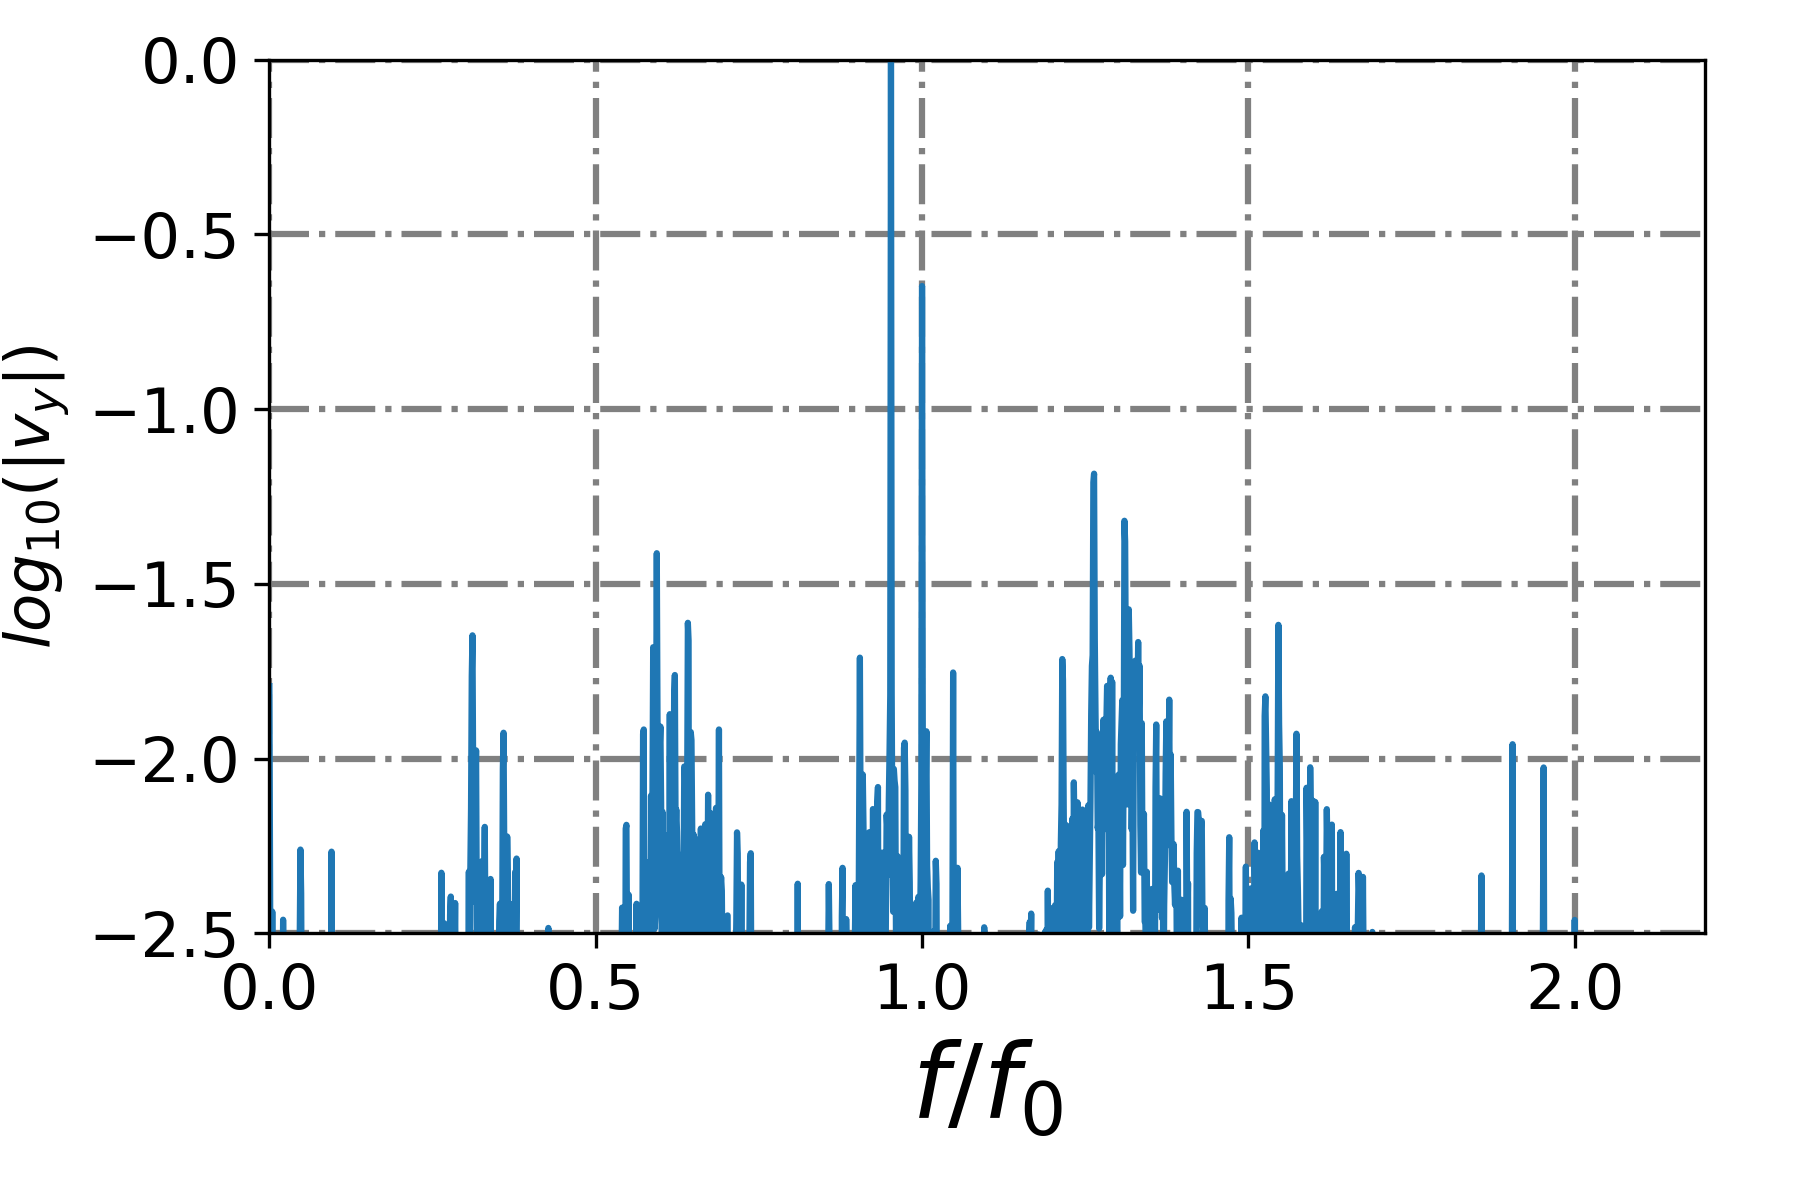
\includegraphics[width=1\textwidth]{pics/H40L60N1ap05dp20w1p63Deltawp05Biharm/spectrumX35p6Y11p2.png}
    \caption{Спектр}
  \end{subfigure}
  \begin{subfigure}[с]{0.45\textwidth}
    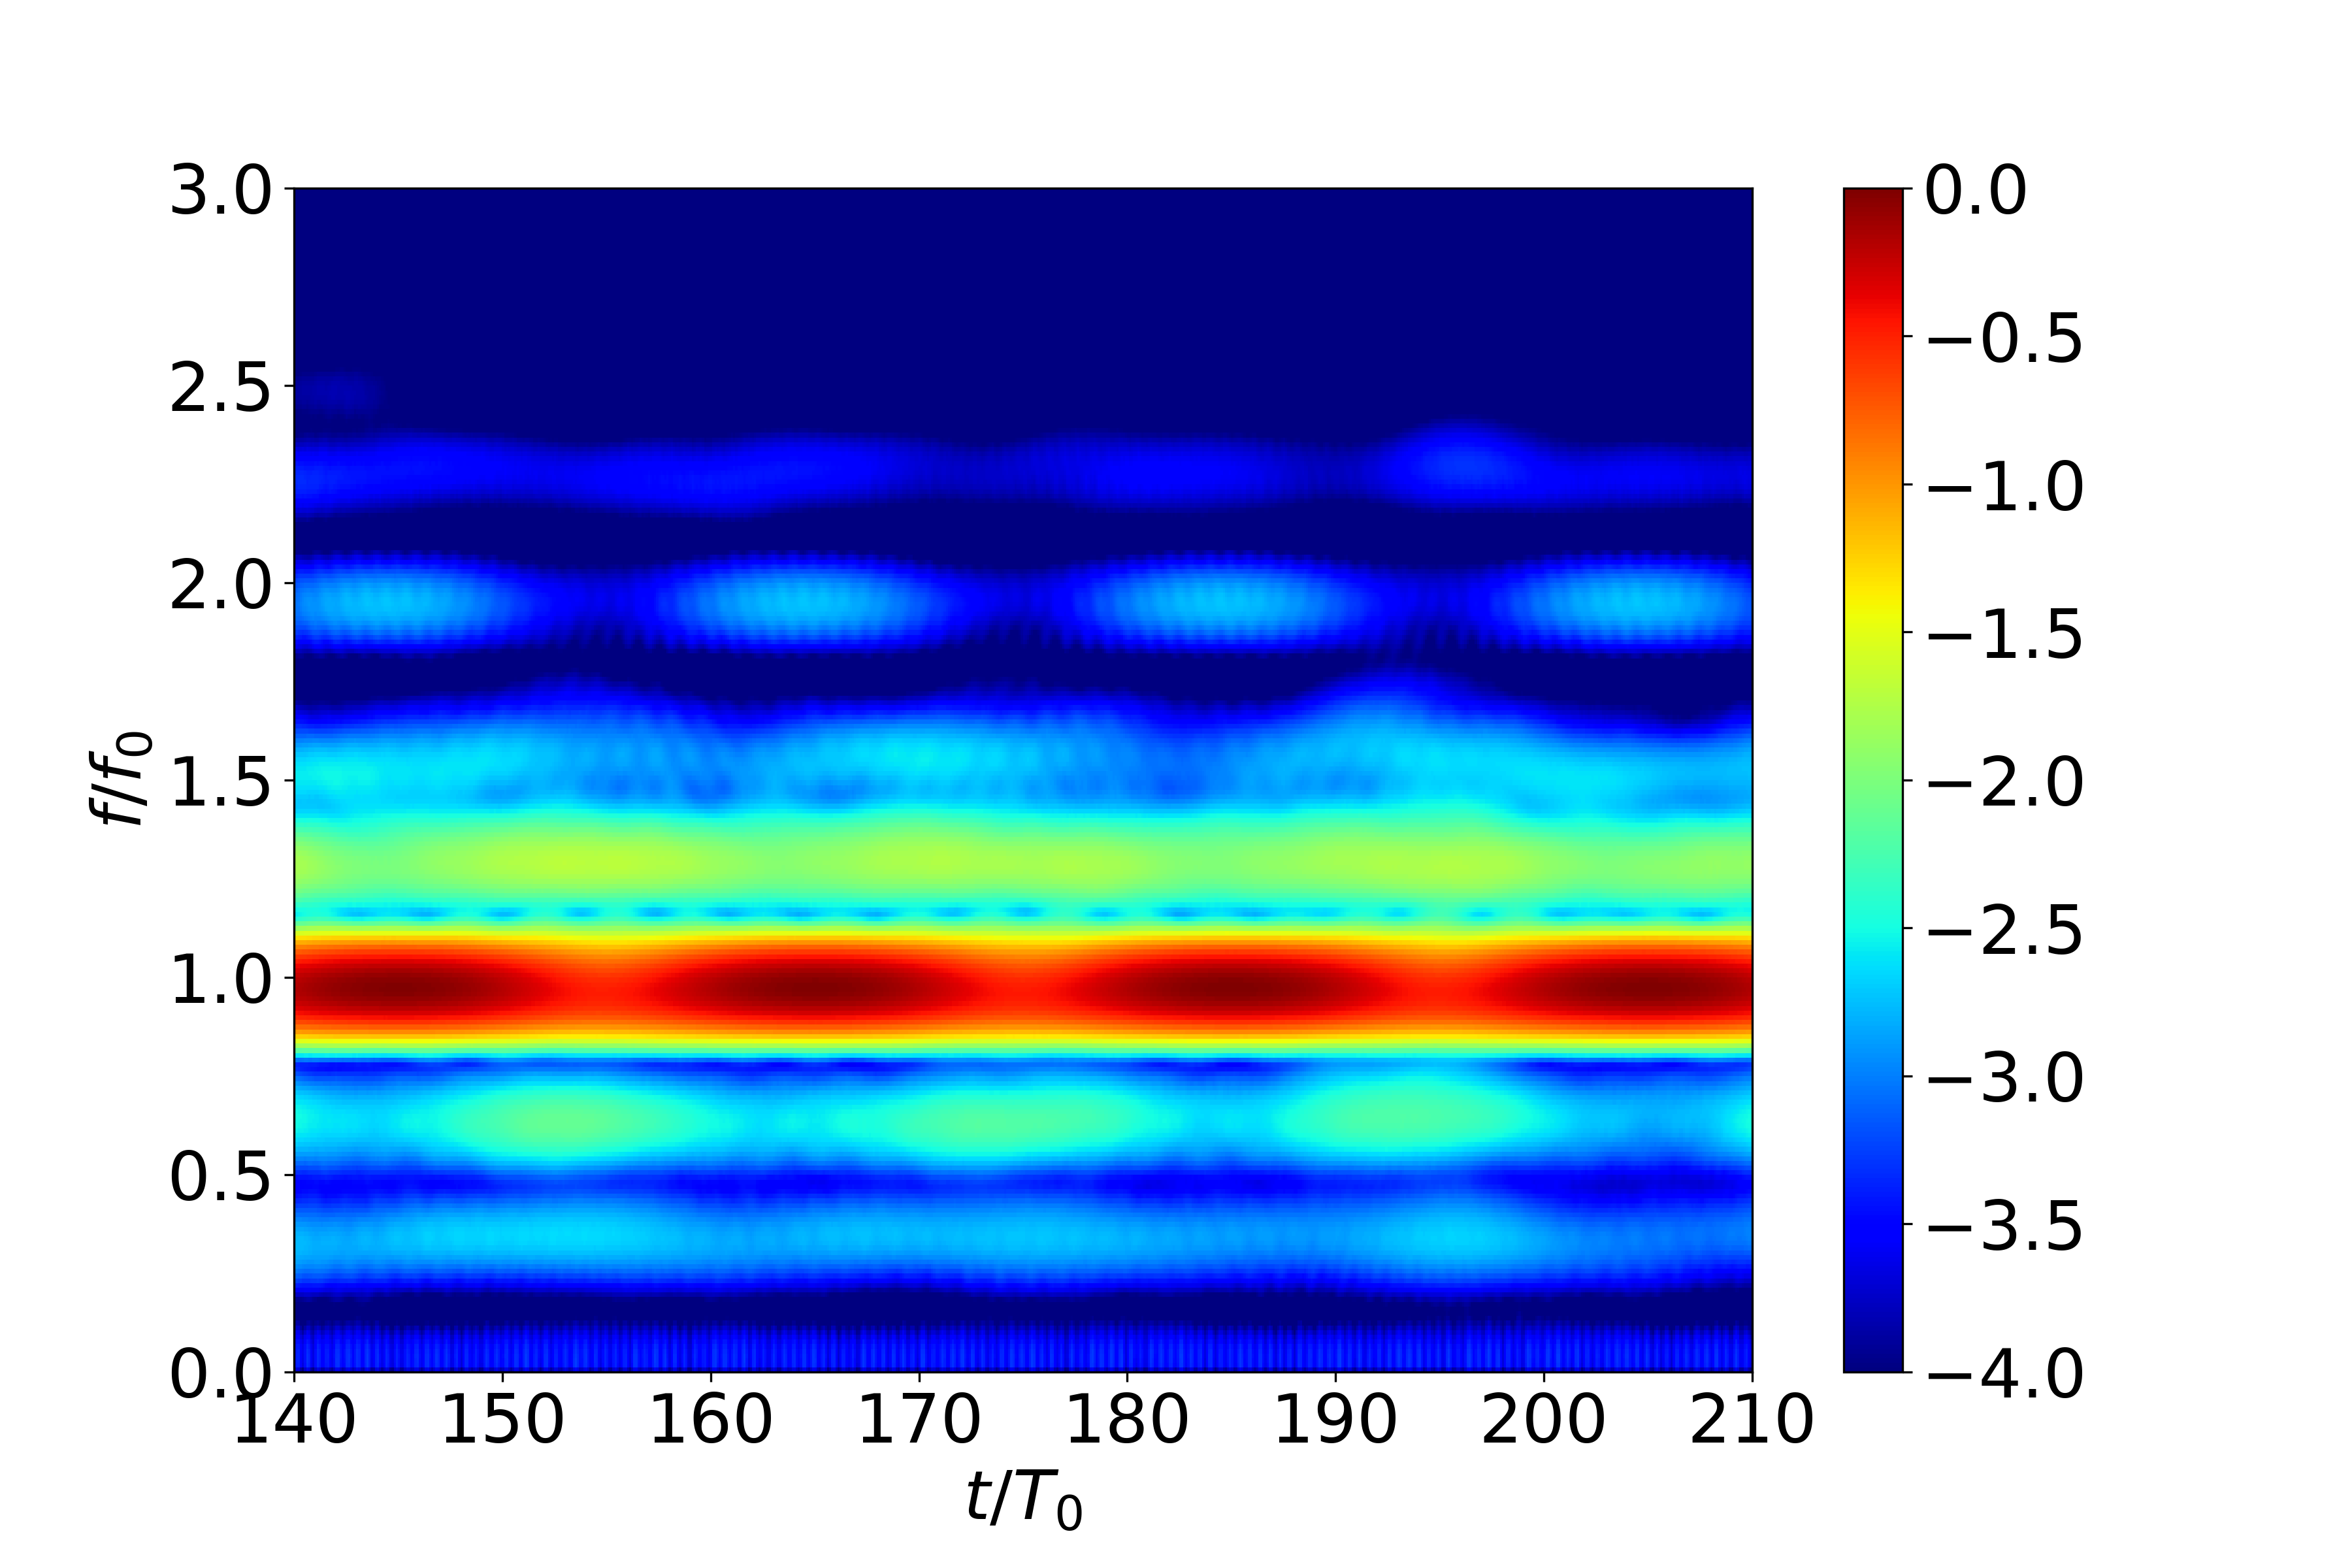
\includegraphics[width=1\textwidth]{pics/H40L60N1ap05dp20w1p63Deltawp05Biharm/TFspectrumX35p6Y11p2N200.png}
    \caption{Частотно-временная диаграмма}
    \label{}
  \end{subfigure}
  \caption{Результаты количественного исследования характеристик течения стратифицированной жидкости в трапециевидном резервуаре при внешнем воздействии с двумя приближенными частотами $\omega_1/N=0.66$ $\omega_2/N=0.68$. Черной линией  на графиках вертикальной скорости и кинетической энергии показана огибающая амплитуды колебаний волнпородуктора.}

  \label{fig:biharmVyap005-1}
\end{figure}

С приближением частот друг к другу(см. рис. \ref{fig:biharmVyap005-2}) появляются дополнительные дочерние волны, но режим успевает стабилизироваться во временной промежуток разности фаз двух частот. 

\begin{figure}
  \centering
  \begin{subfigure}[с]{0.45\textwidth}
    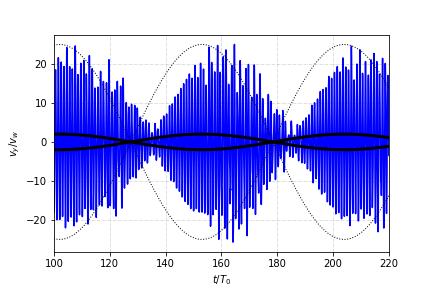
\includegraphics[width=1\textwidth]{pics/H40L60N1ap05dp20w1p63Deltawp02Biharm/vyX35p57Y11p27t4400.png}
    \caption{Вертикальная компонента скорости в зависимости от времени}
  \end{subfigure}
  \begin{subfigure}[с]{0.45\textwidth}
    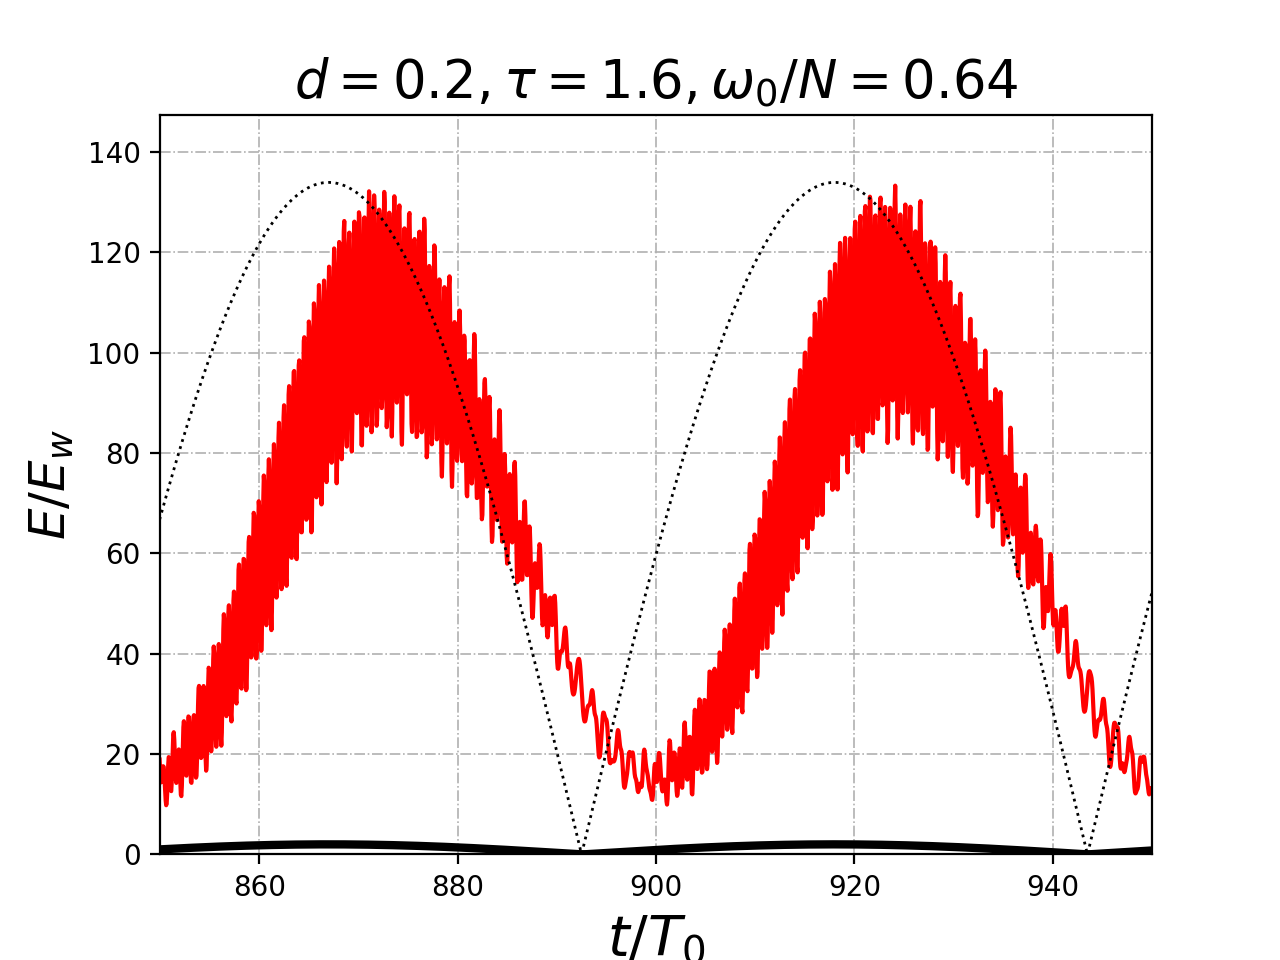
\includegraphics[width=1\textwidth]{pics/H40L60N1ap05dp20w1p63Deltawp02Biharm/2D36x36DiagramH40L60N1ap05dp20w1p63Deltawp02BiharmtotKEnonDim.png}
    \caption{Средняя кинетическая энергия в резервуаре в зависимости от времени}
  \end{subfigure}
  \par
  \begin{subfigure}[с]{0.45\textwidth}
    \includegraphics[width=1\textwidth]{pics/H40L60N1ap05dp20w1p63Deltawp02Biharm/spectrumX35p6Y11p2.png}
    \caption{Спектр}
  \end{subfigure}
  \begin{subfigure}[с]{0.45\textwidth}
    \includegraphics[width=1\textwidth]{pics/H40L60N1ap05dp20w1p63Deltawp02Biharm/TFspectrumX35p6Y11p2N256.png}
    \caption{Частотно-временная диаграмма}
  \end{subfigure}
  \caption{Количественные результаты исследования бигармонического аттрактора внутренних волн с двумя близкими частотами $\omega_1/N=0.628$,  $\omega_2/N=0.641$.}
  \label{fig:biharmVyap005-2}
\end{figure}

Помимо детального анализа результатов моделирования бигармонических аттракторов полученных с помощью метода спектральных элементов, были получены результаты моделирования с помощью метода конечного объема (см. рис. \ref{fig:biharm}). Из рисунка видно, что качественно картина течения совпала с предсказанной при помощи трассировки лучей. 

\begin{figure}
    \centering
    \scalebox{0.95}{
    \begin{tikzpicture}[scale=1.187, z={(-.707,-.5)}]
        \node[anchor=south west,inner sep=0] at (0,0) {\includegraphics[width=\textwidth]{pics/Biharm.png}};
        \draw (0,0,0) -- (12*0.98,0,0) -- (8*0.98,8*0.98,0)--(0,8*0.98,0) --cycle;
        \draw[style = dashed] (9*0.98,0,0)   -- (0,6.4*0.98,0) -- (2.0*0.98,8*0.98,0) -- (5.65*2*0.98,1.4*0.98,0)-- cycle;
        \draw[style = dashed] (0,0.985*2*0.98,0) -- (6.6*0.98,8*0.98,0) -- (9*0.98,6*0.98,0) -- (2.2*0.98,0,0)  -- cycle;
        \draw[thick,->] (9,6,0) -- (11.1,6,0) node[anchor=north east]{$x$};
        \draw[thick,->] (9,6,0) -- (9.1,8,0) node[anchor=north west]{$z$};
    \end{tikzpicture}
    }
    \caption{Поле горизонтальной компоненты скорости для бигармонического аттрактора и трассировка лучей.}
    \label{fig:biharm}
\end{figure}


\section{Кинетическая энергия для монохроматического и бигармонического режимов}

 Для геометрии, показанной на рис.\ref{fig:domainup}, нижняя и верхняя границы диапазона существования аттрактора соответствуют $\omega_{cr1}/N=0.55$ и $\omega_{cr2}/N=0.74$. При достижении этих критических значений частот происходит вырождение параллелограмма в диагональ трапеции. В качестве интегральной размерной меры эффективности генерации аттрактора при постоянной амплитуде волнопродуктора и неизменной форме резервуара принята кинетическая энергия жидкости, проинтегрированная по площади трапеции $S$: $E_{k}(t)=\int_{S}\frac{\rho_{m}}{2}\left[v_{y}^2(t)+v_{x}^2(t)\right]dS$. Для этой меры можно ввести значение, осредненное в скользящем временном окне по достаточно большому числу периодов колебаний $<E_{k}(t)>$, и вариацию относительно среднего, рассчитываемую как $r=D(E_{k}(t)-<E_{k}(t)>)/<E_{k}(t)>$, где $D(E_{k}(t)-<E_{k}(t)>)$ -- дисперсия относительно среднего. Безразмерные величины $\overline{E}_{k}(t)$ и $<\overline{E}_{k}(t)>$ определены путем нормировки на величину $\rho_{m}S(a\omega)^2/2$. Известно, что режимы движения в аттракторах могут быть близки как к прогрессивным, так и к стоячим волнам ~\cite{Brouzetetal2017}. Величина $r$ позволяет дать количественную оценку близости наблюдаемого режима к одному из этих предельных случаев \cite{Brouzetetal2017}. 


Характерный вид зависимостей, наблюдаемых в монохроматическом режиме при малой амплитуде колебаний показан на 

рис. \ref{fig:domainup}
для  $a=0.02$cм ($a/H=5\cdot 10^{-4}$), $\omega/N=0.63$. Характерное время выхода системы на установившийся режим составляет порядка $30$ периодов колебаний, спектр сигнала является с высокой точностью монохроматическим, колебания кинетической энергии относительно среднего имеют небольшую амплитуду ($r=0.103$). За первую ветвь аттрактора принят пучок с наибольшим значением плотности энергии, возникающий после фокусирующего отражения от наклонной стенки. Величины интегральных параметров, характеризующих линейные монохроматические режимы при фиксированном значении $a/H=5\cdot 10^{-4}$ в частотном диапазоне от $\omega_{cr1}/N=0.55$ до $\omega_{cr2}/N=0.74$ приведены в таблице \ref{tab:bolts002}. Видно, что при фиксированной амплитуде колебаний величина кинетической энергии аттрактора максимальна при $\omega/N=0.63$. Очевидно, что при этом значении частоты возмущающего воздействия следует ожидать сильных нелинейных эффектов при увеличении амплитуды колебаний волнопродуктора. Величина $r$ при $\omega/N=0.63$ достигает минимума: движение в аттракторе представлено прогрессивной волной.  Характерные картины течения и зависимости, наблюдаемые в случае слабонелинейного режима при $\omega/N=0.63$ приведены на рис.\ref{fig:Vyamp05} для $a=0.05$см ($a/H=1.25\cdot 10^{-3}$). В слабонелинейном режиме имеет место триадный резонанс \cite{Dauxoisetal2018}, при котором генерируются две дочерние субгармонические волны малой амплитуды.  Частотно-временная диаграмма, показанная на рис. \ref{fig:Vyamp05}, представляет собой спектр сигнала, вычисленный в скользящем окне и осредненный по окрестности точки, лежащей в середине первой ветви аттрактора. Частотный спектр внутренних волн при данном режиме является дискретным, с доминирующим вкладом, соответствующим частоте возмущения $\omega_{0}$, двумя дочерними субгармоническими частотами $\omega_{1}^{*}+\omega_{2}^{*}=\omega_{0}$, двумя супергармоническими частотам $\omega_{1}^{**}=\omega_{1}^{*}+\omega_{0}$, $\omega_{2}^{**}=\omega_{2}^{*}+\omega_{0}$ и удвоенной частотой $2\omega_{0}$. 


\begin{figure}
	\centering
	\begin{subfigure}[с]{0.45\textwidth}
	    \includegraphics[width=1\textwidth]{pics/H40L60N1ap05dp20w0p63/2D36x36DiagramH40L60N1ap05dp20w0p63Vyn00308.png}
	    \caption{Поле вертикальной компоненты скорости при монохроматическом внешнем воздействии с амплитудой($a/H=5\cdot 10^{-4}$)}
	\end{subfigure}
	\begin{subfigure}[с]{0.45\textwidth}
	    \includegraphics[width=1\textwidth]{pics/H40L60N1ap05dp20w0p63/2D36x36DiagramH40L60N1ap05dp20w0p63Pn00308.png}
	    \caption{Поле давления при монохроматическом внешнем воздействии с амплитудой ($a/H=5\cdot 10^{-4}$)}
	\end{subfigure}
	\par
	\begin{subfigure}[с]{0.45\textwidth}
	    \includegraphics[width=1\textwidth]{pics/H40L60N1ap05dp20w0p63/vyX35p57Y11p27t4400.png}
	    \caption{Скорость в середине первого луча аттрактора}
	\end{subfigure}
	\begin{subfigure}[с]{0.45\textwidth}
	    \includegraphics[width=1\textwidth] {pics/H40L60N1ap05dp20w0p63/2D36x36DiagramH40L60N1ap05dp20w0p63totKEnonDim.png}
	    \caption{Кинетическая энергия в середине первого луча аттрактора}
	\end{subfigure}
	\par
	\begin{subfigure}[с]{0.45\textwidth}
	    \includegraphics[width=1\textwidth]{{pics/H40L60N1ap05dp20w0p63/spectrumX35.6Y11.2}.png}
	    \caption{Спектр}
	\end{subfigure}
	\begin{subfigure}[с]{0.45\textwidth}
	    \includegraphics[width=1\textwidth]{{pics/H40L60N1ap05dp20w0p63/TFspectrumX35.6Y11.2N1024}.png}
	    \caption{Частотно-временная диаграмма}
	\end{subfigure}
	\caption{Характерная картина течения при монохроматическом воздействии }
	\label{fig:Vyamp05}
\end{figure}

\begin{table}
	\caption{ Кинетическая энергия при монохроматических воздействиях с амплитудой $a=0.02 cm$}. 
	\begin{center}
		\begin{tabular}{|c|c|c|c|c|c|}
			\hline
			$\displaystyle \frac{\omega_0}{N}$ & $E_k $ &  $<\overline{E}_{k}>$ & r\\
			0.55 ($\omega_{cr,1}$) & $1.32 \cdot 10^{-4}   $& 2.151    & 0.618     \\
			0.58                   & $8.45 \cdot 10^{-4}   $& 12.56    & 0.281     \\
			0.59                   & $ 12  \cdot 10^{-4}   $& 17.33    & 0.3       \\
			0.63                   & $29   \cdot 10^{-4}   $& 36.68    & 0.103     \\
			0.641                  & $23   \cdot 10^{-4}   $& 28.55    & 0.1129    \\
			0.66                   & $13.2 \cdot 10^{-4}   $& 15.14    & 0.152     \\
			0.70                   & $2.84 \cdot 10^{-4}   $& 2.896    & 0.295     \\
			0.74 ($\omega_{cr,2}$) & $1.50 \cdot 10^{-4}   $& 1.356    & 0.215     \\
			\hline
		\end{tabular}
	\end{center}
	\label{tab:bolts002}
\end{table}

При дальнейшем увеличении амплитуды возмущения до $a=0.1$см ($a/H=2.5\cdot 10^{-3}$) происходит развитие каскада триадных взаимодействий. Характерные картины волновых полей, спектров и развития во времени процесса колебаний и кинетической энергии системы приведены на рисунках \ref{fig:Vyamp1}. В частотном спектре сигнала доминируют дискретные компоненты, соответствующие частотам дочерних волн, возникающих при триадном резонансе аналогичные компонентам спектра, возникающим в слабонелинейном случае ($a/H=1.25\cdot 10^{-3}$). При этом полный спектр сигнала представляет собой суперпозицию дискретного и непрерывного спектра. Наличие непрерывного спектра свидетельствует о возникновении режима развитой волновой турбулентности \cite{Brouzet2016,Brouzetetal2017}. Соответствующие характеристики для кинетической энергии системы в сильно нелинейном режиме приведены в таблице \ref{tab:bolts01}. Из сопоставления таблиц \ref{tab:bolts002} и \ref{tab:bolts01} видно, что величины глобальных безразмерных энергетических характеристик системы (средней энергии  $<\overline{E}_{k}>$ и вариации относительно среднего $r$) в случае режима развитой волновой турбулентности слабо отличаются от безразмерных величин, характерных для линейного режима. Сопоставление волновых картин в линейном и нелинейном случаях показывает, что во втором случае энергия более равномерно распределена по изучаемой области: ветви аттрактора имеют большую ширину, а дочерние волны заполняют все пространство.

\begin{table}
	\caption{  Кинетическая энергия при монохроматических воздействиях с амплитудной $a=0.1 cm$. }
	\begin{center}
		\begin{tabular}{|c|c|c|c|c|}
			\hline
			$\displaystyle \frac{\omega_0}{N}$ & $E_k (erg)$ &  $<\overline{E}_{k}>$  & r\\
			%          $a$ &    $\displaystyle \frac{\omega_0}{N}$   & $E_k$ & ${E_k}/{\frac{(a\omega_0)^2}{2}}$ & $D_k$ & r\\
			0.55 ($\omega_{cr,1}$) & $33.0 \cdot 10^{-4}              $& 2.14  & 0.6193     \\
			0.63                   & $725 \cdot 10^{-4}              $& 36.7  & 0.1346     \\
			0.74 ($\omega_{cr,2}$) & $37.0 \cdot 10^{-4}              $& 1.35  & 0.2192     \\
			\hline
		\end{tabular}
	\end{center}
	\label{tab:bolts01}
\end{table}

Характерный пример волновой картины и основных качественных и количественных характеристик системы в линейном случае при бигармоническом внешнем воздействии приведен на рис.\ref{fig:biharmVyamp02} для следующих значений параметров: $\omega_1/N=0.58, \omega_2/N=0.66, a=0.02$см. Видно, что система выходит на режим квазистационарных биений за время порядка $40$ периодов колебаний, что близко к характерному времени выхода на процесс стационарных колебаний в монохроматическом случае. На частотном спектре доминируют пики, соответствующие частотам внешнего возмущения, имеются также пики, соответствующие частоте  $2\omega_1/N$ и разностной частоте $(\omega_2-\omega_1)/N$, но их величина более чем на два порядка меньше основного пика. Моменты времени, соответствующие максимальным значениям кинетической энергии, существенно отстают от моментов времени, соответствующих максимальным значениям амплитуды колебаний волнпродуктора. Важно отметить, что после выхода системы на режим установившихся биений средняя кинетическая энергия системы, возбуждаемой бигармоническим возмущением, с высокой точностью равна сумме энергий аттракторов, возбуждаемых монохроматическими возмущениями по отдельности $\overline{E}_{k}= { 21.7 \cdot 10^{-4}  }\approx \overline{E}_{k1}+\overline{E}_{k2}= (8.45+13.2) \cdot 10^{-4} = 21.65 \cdot 10^{-4}\, (erg/cm^2) $. Таким образом, в линейном режиме с высокой точностью соблюдается принцип линейной суперпозиции, что выполняется также при малой разности частот $(\omega_1-\omega_2)/N$. 

Примеры нелинейной динамики волновых аттракторов, генерируемых бигармоническими колебаниями волнопродуктора приведены на рис. \ref{fig:biharmVyap005-1} %\ref{fig:biharmVyap005-1-1} 
($\omega_1/N=0.66$, $\omega_2/N=0.628$, $\delta \omega/N=0.031$) и \ref{fig:biharmVyap005-2}, 
%\ref{fig:biharmVyap005-2-1} 
($\omega_1/N=0.628$, $\omega_2/N=0.641$, $\delta \omega/N=0.013$). Во всех случаях амплитуды колебаний волнопродуктора составили $a_{1}=a_{2}=0.05$см. Можно видеть, что в обоих случаях формируется движение, для которого характерен сложный частотный спектр, причем при уменьшении расстройки частот $\delta \omega$ наблюдается тенденция к более густому <<заселению>> спектра.  На графиках зависимости вертикальной скорости от времени виден характерный процесс <<биений>>. График зависимости кинетической энергии системы от времени показывает, что помимо колебаний среднего значения энергии имеет место нетривиальная динамика высокочастотных пульсаций энергии: на фазах роста и убывания огибающей амплитуды колебаний волнопродуктора амплитуды пульсаций могут отличаться на порядок. Таким образом, для нелинейного бигармонического режима характерны периодические <<вспышки>> волновой турбулентности. Такие <<вспышки>> хорошо видны на частотно-временных диаграммах, приведенных на рис.  \ref{fig:biharmVyap005-1} и \ref{fig:biharmVyap005-2}. В частности, на частотно-вереиенной диаграмме, приведенной на рис.  \ref{fig:biharmVyap005-1}, можно видеть, что <<биения>> амплитуды сигнала на частоте, близкой к частоте возмущающего воздействия, сдвинуты по времени относительно <<биений>> дочерних волн. Таким образом, <<биения>> огибающей колебаний волнопродуктора, <<биения>> средней кинетической энергии и <<вспышки>> волновой турбулентности рассогласованны между собой по времени. Можно предположить, что и в природных системах имеется рассогласование по времени между огибающей амплитуды внутреннего прилива и интенсификацией внутренней волновой турбулентности и перемешивания. Предварительное исследование энергии аттракторов, генерируемых бигармоническим возмущением, показывает, что в нелинейном случае средняя энергия системы существенным образом отличается от суммы энергий составляющих.  

%
%\backmatter %% Здесь заканчивается нумерованная часть документа и начинаются ссылки и
%            %% заключение
\chapter{Заключение}
\label{cha:Conclusion}

%Заключение последовательное логически стройное изложение итогов исследования в соответствии с целью и задачами, поставленными и сформулированными во введении. В нем содержатся выводы и определяются дальнейшие перспективы работы.

% \begin{itemize}
%     \item В ходе работы определена целесообразность использования метода конечного объема для моделирования аттракторов внутренних волн.
%     \item Найдены теоретические диапазоны частот колебаний волнопродуктора, которые способны порождать аттракторы.
%     \item Установлено, что при воздействии на резервуар со стратифицированной жидкостью волнопродуктором, который совершает колебания описываемые суммой двух монохроматических функций образуется суперпозиция двух аттракторов в одном резервуаре.
%     \item Обнаружено, что при близости частот двух монохроматических функций возбуждающих внутренние волны в резервуаре образуются амплитудные биения. 
% \end{itemize}



Показано, что результаты моделирования аттракторов внутренних волн, полученные с помощью методов конечного объёма при увеличении количества ячеек стремятся к результатам, полученным с помощью метода высокого порядка. Таким образом сделан вывод о целесообразности дальнейшего использования конечно объёмной реализации квазигидродинамических уравнений для моделирования аттракторов внутренних волн. 
Аналитически определены  границы частотного диапазона существования аттрактора. Выведены формулы расчёта каждой из границ в зависимости от геометрических характеристик резервуара и частоты плавучести.


Получены результаты моделирования бигармонических аттракторов, то есть таких, которые возникают при воздействии на жидкость в трапециевидном резервуаре с двумя частотами, попадающими в интервал существования аттрактора. Установлено, что в этом случае картина течения каждой частоты по отдельности накладывается друг на друга. В резервуаре появляются два независимых аттрактора, каждый из которых совершает движение с собственной частотой, а взаимодействуют они только в точках пересечения. 


Рассмотрены различные комбинации частот из диапазона существования аттракторов. Когда частоты совпадают, это фактически удваивает амплитуду колебаний волнопродуктора монохроматического аттрактора. В случае большой амплитуды колебаний волнопродуктора аттрактор начинает поражать дочерние волны и насыщает спектр. В случае разнесённых частот аттракторы практически не взаимодействуют, амплитуды не складываются. В случае, когда частоты приближены друг к другу, в момент совпадения фаз наблюдается взаимодействие аттракторов, тогда постепенно спектр частот начинает насыщаться, но в момент разности фаз спектр возвращается в исходное состояние. В случае, когда частоты располагаются еще ближе друг к другу, на частотно-временной диаграмме наблюдается еще более активное взаимодействие аттракторов, а на графике зависимости средней кинетической энергии в резервуаре от времени наблюдаются биения.


Выяснено, что с большой точностью сумма средних кинетических энергий аттракторов, образующихся при монохроматическом режиме колебаний волнопродуктора, равна средней кинетической энергии бигармонического аттрактора.

Работа представляет собой первый шаг к моделированию аттракторов как природного явления в океане. Для этого необходимо разработать инструменты численного моделирования монохроматического аттрактора в условиях геометрии, приближенной к реальной. А также исследовать течения возникающие при воздействии на стратифицированную жидкость суммой нескольких монохроматических колебаний. 

Для реализации инструмента численного моделирования в сложной геометрии была разработана программа, которая подлежала государственной регистрации номер 2018663951. Разработанный инструмент имеет ряд преимуществ относительно уже существующих программных средств, такие как точность, гибкость, возможность встроить дополнительные модули физических процессов и возможность работать со сложной геометрией на неортогональных сетках. Количественное соответствие результатов моделирования методом конечного объема и методом спектральных элементов показывают целесообразность дальнейшего развития метода конечного объема на базе квазигидродинамических уравнений. Соответствие предсказанной трассировкой лучей формы бигармонического аттрактора и результатов моделирования с помощью регуляризованных уравнений дает возможность сделать заключение о целесообразности дальнейшего применения. 

Количественное исследование показало, что после выхода системы на режим установившихся колебаний средняя кинетическая энергия системы, возбуждаемой бигармоническим возмущением, с высокой точностью равна сумме энергий аттракторов, возбуждаемых монохроматическими возмущениями по отдельности. Таким образом, в линейном режиме с высокой точностью соблюдается принцип линейной суперпозиции, что выполняется также при малой разности частот. 

В нелинейном случае средняя энергия системы существенным образом отличается от суммы энергий составляющих. Наблюдается режим <<биений>> сопровождающийся <<вспышками>> волновой турбулентности, возникающей вследствие каскада триадных взаимодействий. При этом уровень пульсаций кинетической
энергии на фазе роста огибающей амплитуды волнопродуктора, может на порядок превышать уровень, соответствующий спаду амплитуды колебаний волнопродуктора.


Реализован квазигидродинамический подход на базе конечно объёмного пакета OpenFOAM. Программа охватывает дозвуковой и трансзвуковой диапазон скоростей, позволяет проводить численное моделирование вязких течений с переносом. Исходный код, тестовые примеры и документация размещена в открытом хранилище исходного кода на github. 

% % Список литературы при помощи BibTeX
% Юзать так:
%
% pdflatex rpz
% bibtex rpz
% pdflatex rpz

%\bibliographystyle{gost780u}
%\bibliographystyle{plain}
%\bibliographystyle{ugost2008ns}
\bibliographystyle{ugost2008}
\bibliography{rpz}

%%% Local Variables: 
%%% mode: latex
%%% TeX-master: "rpz"
%%% End: 

%% % Список литературы при помощи BibTeX
% Юзать так:
%
% pdflatex rpz
% bibtex rpz
% pdflatex rpz

%\bibliographystyle{gost780u}
%\bibliographystyle{plain}
%\bibliographystyle{ugost2008ns}
\bibliographystyle{ugost2008}
\bibliography{rpz}

%%% Local Variables: 
%%% mode: latex
%%% TeX-master: "rpz"
%%% End: 


%\appendix   % Тут идут приложения

\end{document}

%%% Local Variables:
%%% mode: latex
%%% TeX-master: t
%%% End:
